%% iccp20_template.tex
%% Created by Ayan Chakrabarti from the IEEE bare_jrnl_compsoc.tex file.
%%
%% bare_jrnl_compsoc.tex
%% V1.4b
%% 2015/08/26
%% by Michael Shell
%% See:
%% http://www.michaelshell.org/
%% for current contact information.
%%
%% This is a skeleton file demonstrating the use of IEEEtran.cls
%% (requires IEEEtran.cls version 1.8b or later) with an IEEE
%% Computer Society journal paper.
%%
%% Support sites:
%% http://www.michaelshell.org/tex/ieeetran/
%% http://www.ctan.org/pkg/ieeetran
%% and
%% http://www.ieee.org/

%%*************************************************************************
%% Legal Notice:
%% This code is offered as-is without any warranty either expressed or
%% implied; without even the implied warranty of MERCHANTABILITY or
%% FITNESS FOR A PARTICULAR PURPOSE! 
%% User assumes all risk.
%% In no event shall the IEEE or any contributor to this code be liable for
%% any damages or losses, including, but not limited to, incidental,
%% consequential, or any other damages, resulting from the use or misuse
%% of any information contained here.
%%
%% All comments are the opinions of their respective authors and are not
%% necessarily endorsed by the IEEE.
%%
%% This work is distributed under the LaTeX Project Public License (LPPL)
%% ( http://www.latex-project.org/ ) version 1.3, and may be freely used,
%% distributed and modified. A copy of the LPPL, version 1.3, is included
%% in the base LaTeX documentation of all distributions of LaTeX released
%% 2003/12/01 or later.
%% Retain all contribution notices and credits.
%% ** Modified files should be clearly indicated as such, including  **
%% ** renaming them and changing author support contact information. **
%%*************************************************************************


\documentclass[10pt,journal,compsoc]{IEEEtran}
\newif\ifpeerreview

%%% Important: for camera ready submissions, replace the following line
%%% with \peerreviewfalse
\peerreviewfalse


\usepackage[nocompress]{cite}
\usepackage{url}
\usepackage{amsmath,amssymb,graphicx, mathtools}
\usepackage{multirow}
\usepackage{booktabs}

\usepackage{lipsum} % Only used to generate random text.

\usepackage{subfig}
\usepackage{hyperref}
\hypersetup{
    colorlinks=true,
    linkcolor=blue,
    filecolor=magenta,      
    urlcolor=cyan,
    pdftitle={Overleaf Example},
    pdfpagemode=FullScreen,
    }
\urlstyle{same}

\usepackage[switch]{lineno}

% customized style
\usepackage{customized}

% Insert your paper ID and information below
\newcommand{\paperID}{XXXX}

% Enter your paper title below
\title{Vax Populi: COVID-19 Outcomes and Political Alignment in New York City}

% Enter your author information before
% Note this is only necessary for the camera review. Submissions are anonymized.
\author{John Lin% <-this % stops a space
% \IEEEcompsocitemizethanks{\IEEEcompsocthanksitem M. Shell is with the Department
% of Electrical and Computer Engineering, Georgia Institute of Technology, Atlanta,
% GA, 30332.\protect\\
% % note need leading \protect in front of \\ to get a newline within \thanks.
% E-mail: see http://www.michaelshell.org/contact.html
% \IEEEcompsocthanksitem J. Doe is with Anonymous University.}% <-this % stops an unwanted space
}


\begin{document}

\IEEEtitleabstractindextext{%
% \begin{abstract}
% The abstract goes here. \lipsum[1]
% \end{abstract}

\begin{IEEEkeywords} % Enter keywords here
COVID-19, NYC Health Data, Vaccination, Politics, Election Data
\end{IEEEkeywords}
}


% Make Title
\ifpeerreview
\linenumbers \linenumbersep 15pt\relax 
\author{Paper ID \paperID\IEEEcompsocitemizethanks{\IEEEcompsocthanksitem This paper is under review for ICCP 2020 and the PAMI special issue on computational photography. Do not distribute.}}
\markboth{Anonymous ICCP 2020 submission ID \paperID}%
{}
\fi
\maketitle



% The first section title should be wrapped inside a \IEEEraisesectionheading as follows.
\IEEEraisesectionheading{
  \section{Introduction}\label{sec:introduction}
}
% The very first letter of the paper is a 2 line initial drop letter
% followed by the rest of the first word in caps.
% 
% form to use if the first word consists of a single letter:
% \IEEEPARstart{A}{demo} file is ....
% 
% form to use if you need the single drop letter followed by
% normal text (unknown if ever used by the IEEE):
% \IEEEPARstart{A}{}demo file is ....
% 
% Some journals put the first two words in caps:
% \IEEEPARstart{T}{his demo} file is ....
% 
% Here we have the typical use of a "T" for an initial drop letter
% and "HIS" in caps to complete the first word.
The COVID-19 pandemic has affected communities across the globe with wide-reaching impacts on public health and socioeconomic consequences. However, the question arises: did the pandemic affect everyone equally? This project aims to explore the disparities in COVID-19 outcomes across different communities, with a particular focus on New York City (NYC).

New York City was chosen for this study due to its unique characteristics - it serves as a microcosm of various demographic and cultural differences, making it an ideal location to study the intersection of public health and socio-political factors. NYC is well-connected through public transit and other transport options, which facilitates the spread of infectious diseases. Additionally, the city is composed of distinct communities, each with its own demographic and cultural profile.

The recent 2024 US election has highlighted heightened polarity on various issues, including healthcare administration and policy. This polarization raises an important question: does political affiliation stratify health outcomes, particularly in the context of COVID-19? The anti-vaccination movement, for instance, has often been framed as a political issue. This project seeks to examine whether political affiliation correlates with COVID-19 outcomes, such as case rates, vaccination rates, and death rates, in NYC neighborhoods.

By analyzing COVID-19 outcomes in relation to election voting ratios per district for the 2020 and 2024 elections, we hope to uncover patterns that highlight issues in public health within diverse urban populations. This analysis aims to provide insights into how political and social factors may influence public health outcomes, and to identify potential areas for targeted public health interventions.
% \begin{figure}[!t]
% \centering
% \framebox[\columnwidth]{\parbox{0.9\columnwidth}{~\\~\\~\\~\\~\\}}
% \caption{Example one-column figure.}
% \end{figure}


\section{Methods}
\subsection{Datasets}
\subsubsection{NYC COVID Data}

The NYC COVID Data dataset \cite{coviddatanyc} is publicly available on GitHub and is maintained by the NYC Department of Health. This dataset provides comprehensive information on the impact of COVID-19 across New York City's neighborhoods. The data is organized using Modified Zip Code Tabulation Areas (MODZCTA), which allows for detailed spatial analysis.

Key features of the dataset include:
\begin{itemize}
    \item \textbf{Case Counts}: The total number of confirmed COVID-19 cases in each neighborhood.
    \item \textbf{Case Rates}: The rate of confirmed COVID-19 cases per 100,000 residents, providing a normalized measure of infection spread.
    \item \textbf{Death Counts}: The total number of confirmed COVID-19 related deaths in each neighborhood.
    \item \textbf{Death Rates}: The rate of confirmed COVID-19 related deaths per 100,000 residents, offering a normalized measure of mortality.
\end{itemize}

To facilitate analysis, we perform some post-processing on the dataset: normalizing the case rates and death rates to a floating-point number between 0 and 1. This allows cases to be represented as percentages of the total population in that neighborhood.

\subsubsection{NYC COVID Vaccination Data}

The NYC COVID Vaccination Data dataset \cite{vaxdatanyc} is publicly available on GitHub and is maintained by the NYC Department of Health. This dataset provides detailed information on COVID-19 vaccination rates across New York City's neighborhoods. Similar to the COVID case data, this dataset uses Modified Zip Code Tabulation Areas (MODZCTA) for spatial organization.

Key features of the dataset:
\begin{itemize}
    \item \textbf{Vaccination Rates}: The dataset includes cumulative vaccination rates as percentages of the total population in each neighborhood.
    \item \textbf{Stratified Data}: The data is stratified into different categories:
    \begin{itemize}
        \item Individuals vaccinated with only the first dose.
        \item Individuals who are fully vaccinated (two or more doses).
        \item Individuals who have received additional doses (more than two doses).
    \end{itemize}
\end{itemize}

To facilitate analysis, we focused on post-processing the following features:
\begin{itemize}
    \item \textbf{Full Vaccination Rates}: We primarily focus on the percentage of individuals who are fully vaccinated (two or more doses), as this aligns with popular policy definitions of a complete vaccination program.
    \item \textbf{Normalization}: Similar to the COVID case data, we normalize the vaccination rates to a floating-point number between 0 and 1, representing the percentage of the total population in each neighborhood.
\end{itemize}

\subsubsection{NYC Electoral Districts}

The NYC Electoral Districts dataset \cite{nycelectoraldistricts} provides detailed information on the boundaries of electoral districts within New York City. This dataset is essential for understanding the political landscape of NYC and is available from the NYC Planning website.

Key features of the dataset include:
\begin{itemize}
    \item \textbf{Electoral Boundaries}: The dataset includes the geographic delineations of various political districts, such as congressional, state senate, and state assembly districts.
    \item \textbf{Shapefile Format}: The data is provided in shapefile format, which includes polygon geometry for precise mapping and spatial analysis.
    \item \textbf{District Numbers}: Each electoral division is identified by its district number, facilitating detailed and organized analysis.
\end{itemize}

\subsubsection{NYC Election Results 2020 and 2024}

The NYC Election Results dataset, created by Todd W. Schneider and available on GitHub \cite{nycelectionmap}, provides detailed election results for New York City during the 2016, 2020, and 2024 presidential elections. This dataset is essential for analyzing the political landscape of NYC and its potential impact on COVID-19 outcomes.

Key features of this dataset include:
\begin{itemize}
    \item \textbf{Election Results}: The dataset includes the number of votes cast for the Democratic (Dem) and Republican (GOP) candidates in each electoral district.
    \item \textbf{Temporal Data}: The dataset covers three election years: 2016, 2020, and 2024. This allows for comparative analysis of voting patterns over time.
    \item \textbf{Geographic Mapping}: The election results are matched with electoral district codes, facilitating geographic analysis.
\end{itemize}

We also perform some post-processing on this dataset by:
\begin{itemize}
    \item \textbf{Filtering by Year}: We primarily focus on the 2020 election results, as this year coincides with the peak of the COVID-19 pandemic. However, we also consider the 2024 election results to examine changes in voting patterns and correlations over time.
    \item \textbf{Data Integration}: We integrate the election results with the COVID-19 and vaccination datasets based on electoral district codes.
    \item \textbf{Normalization}: We normalize the voting data to represent the proportion of votes for each candidate as a floating-point number between 0 and 1. Since we are mostly focused on Dem vs. GOP voting ratios, we sum the votes for both parties, and take the fraction of each as Democrat-two-party and Republican-two-party fractions.
\end{itemize}

\subsection{Data transformation and cleaning}

The data transformation and cleaning process is one of the most computationally intensive parts of this project. It involves several steps to ensure that the datasets are properly aligned and ready for analysis.

\subsubsection{Geographic Data Integration}
\begin{itemize}
    \item \textbf{MODZCTA Regions}: The NYC COVID data and vaccination data are organized by Modified Zip Code Tabulation Areas (MODZCTA), which consist of 177 regions. (Fig. \ref{modzcta})
    \item \textbf{Electoral Districts}: The NYC electoral districts dataset contains 4345 distinct regions. These regions are represented as shapefiles with polygon geometry. (Fig. \ref{nyed})
    \item \textbf{Spatial Join}: Using geographic information system (GIS) tools, we perform a spatial join to combine the MODZCTA regions with the electoral districts. This results in a polygon map with 177 regions, closely matching the MODZCTA regions. (Fig. \ref{merged})
\end{itemize}

\begin{figure*}
    \centering
    \subfloat[NYC MODZCTA]{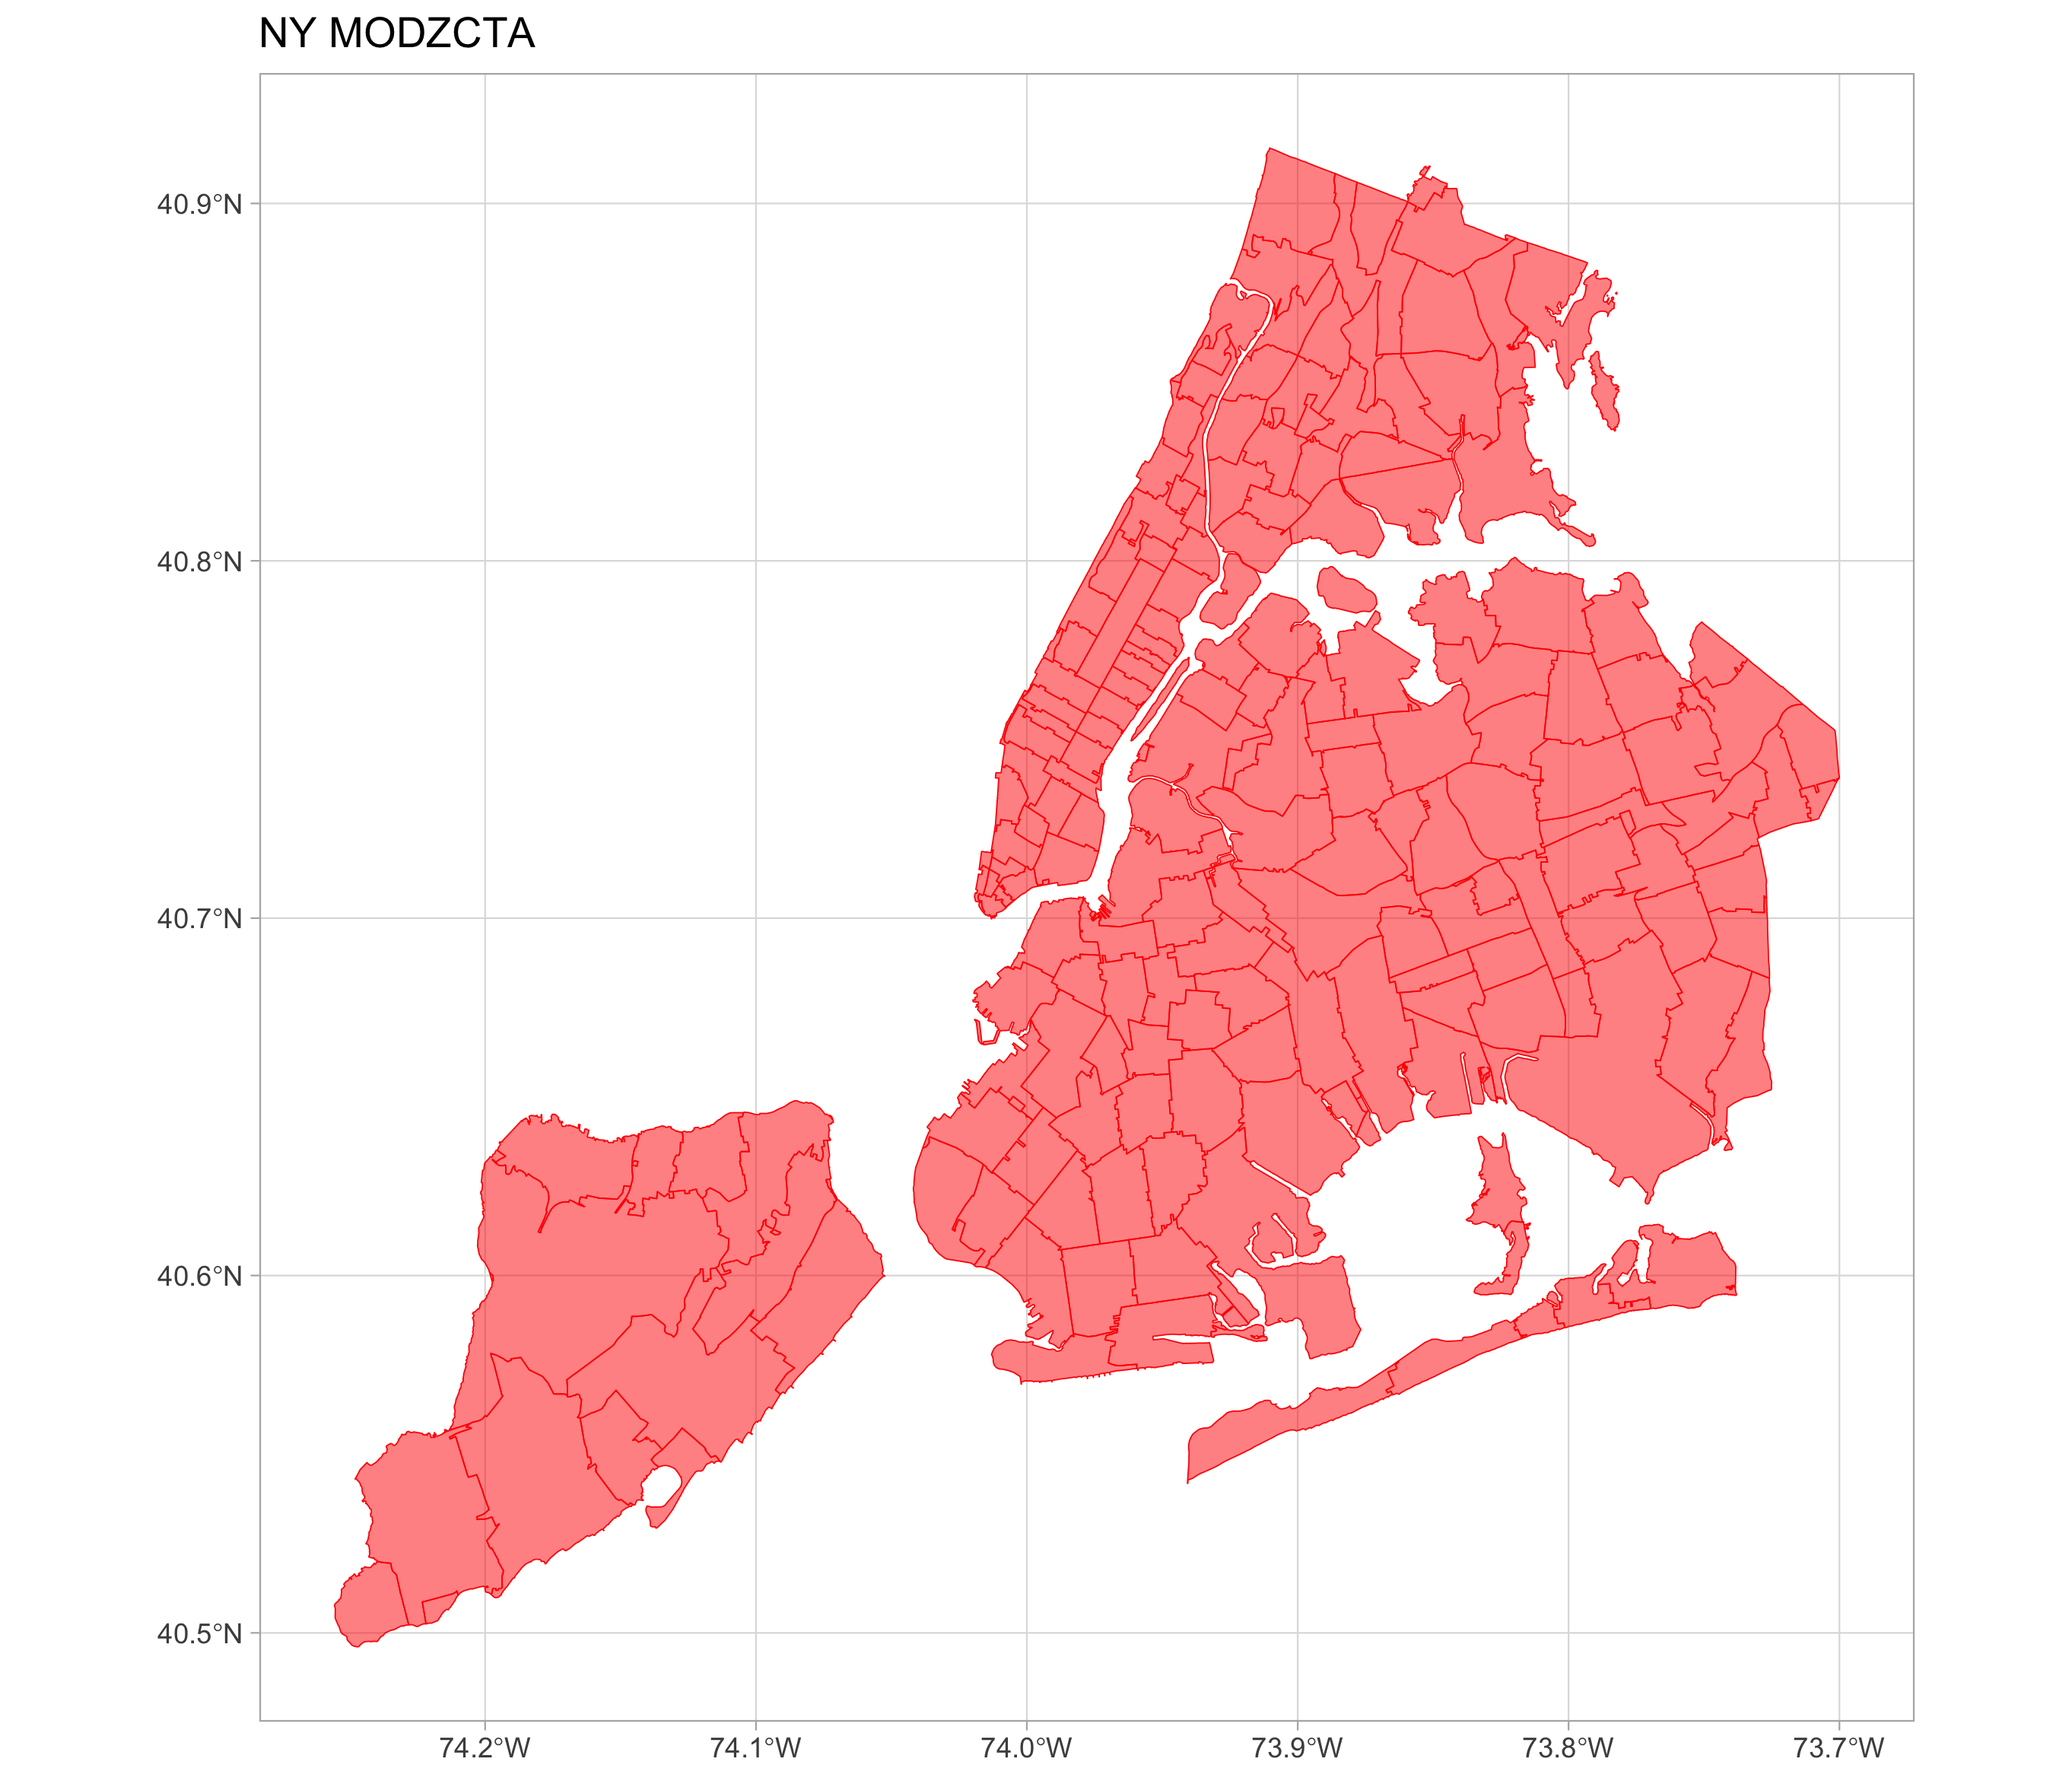
\includegraphics[width=0.3\linewidth]{out/eda/modzcta_gg.png}\label{modzcta}}
    \subfloat[NYC Electoral Districts]{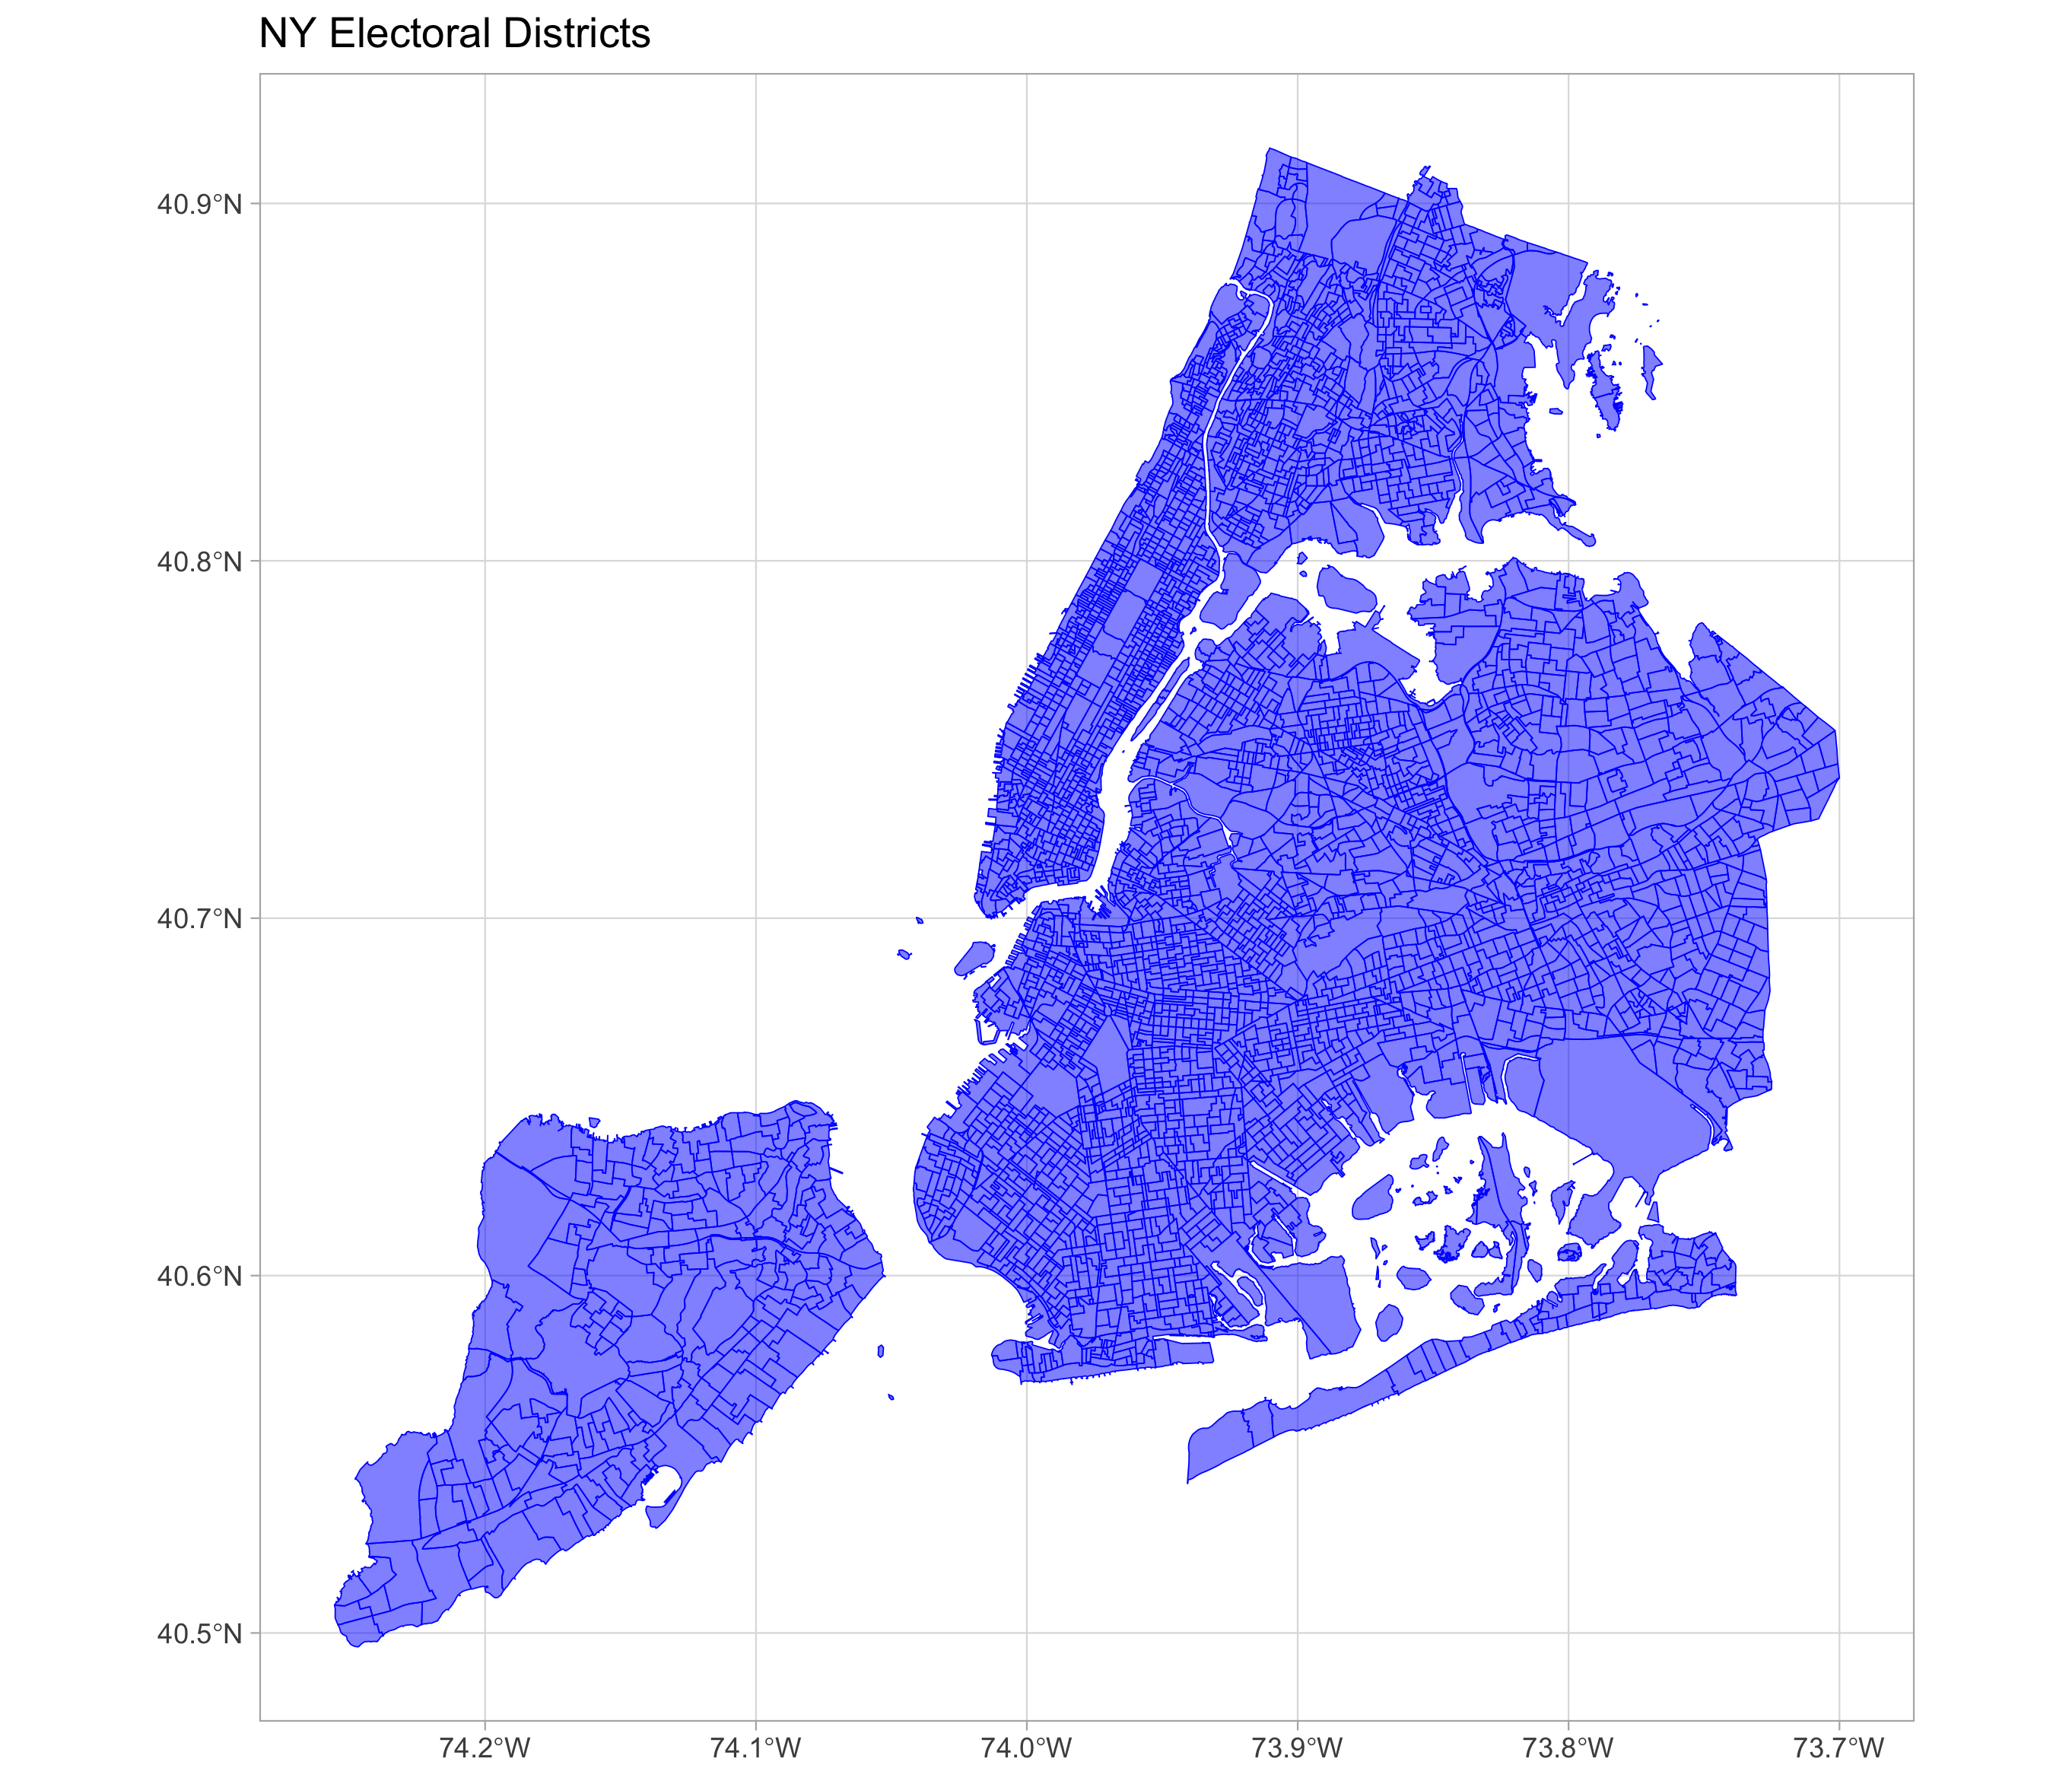
\includegraphics[width=0.3\linewidth]{out/eda/nyed_gg.png}\label{nyed}}
    \subfloat[Merged through spatial join]{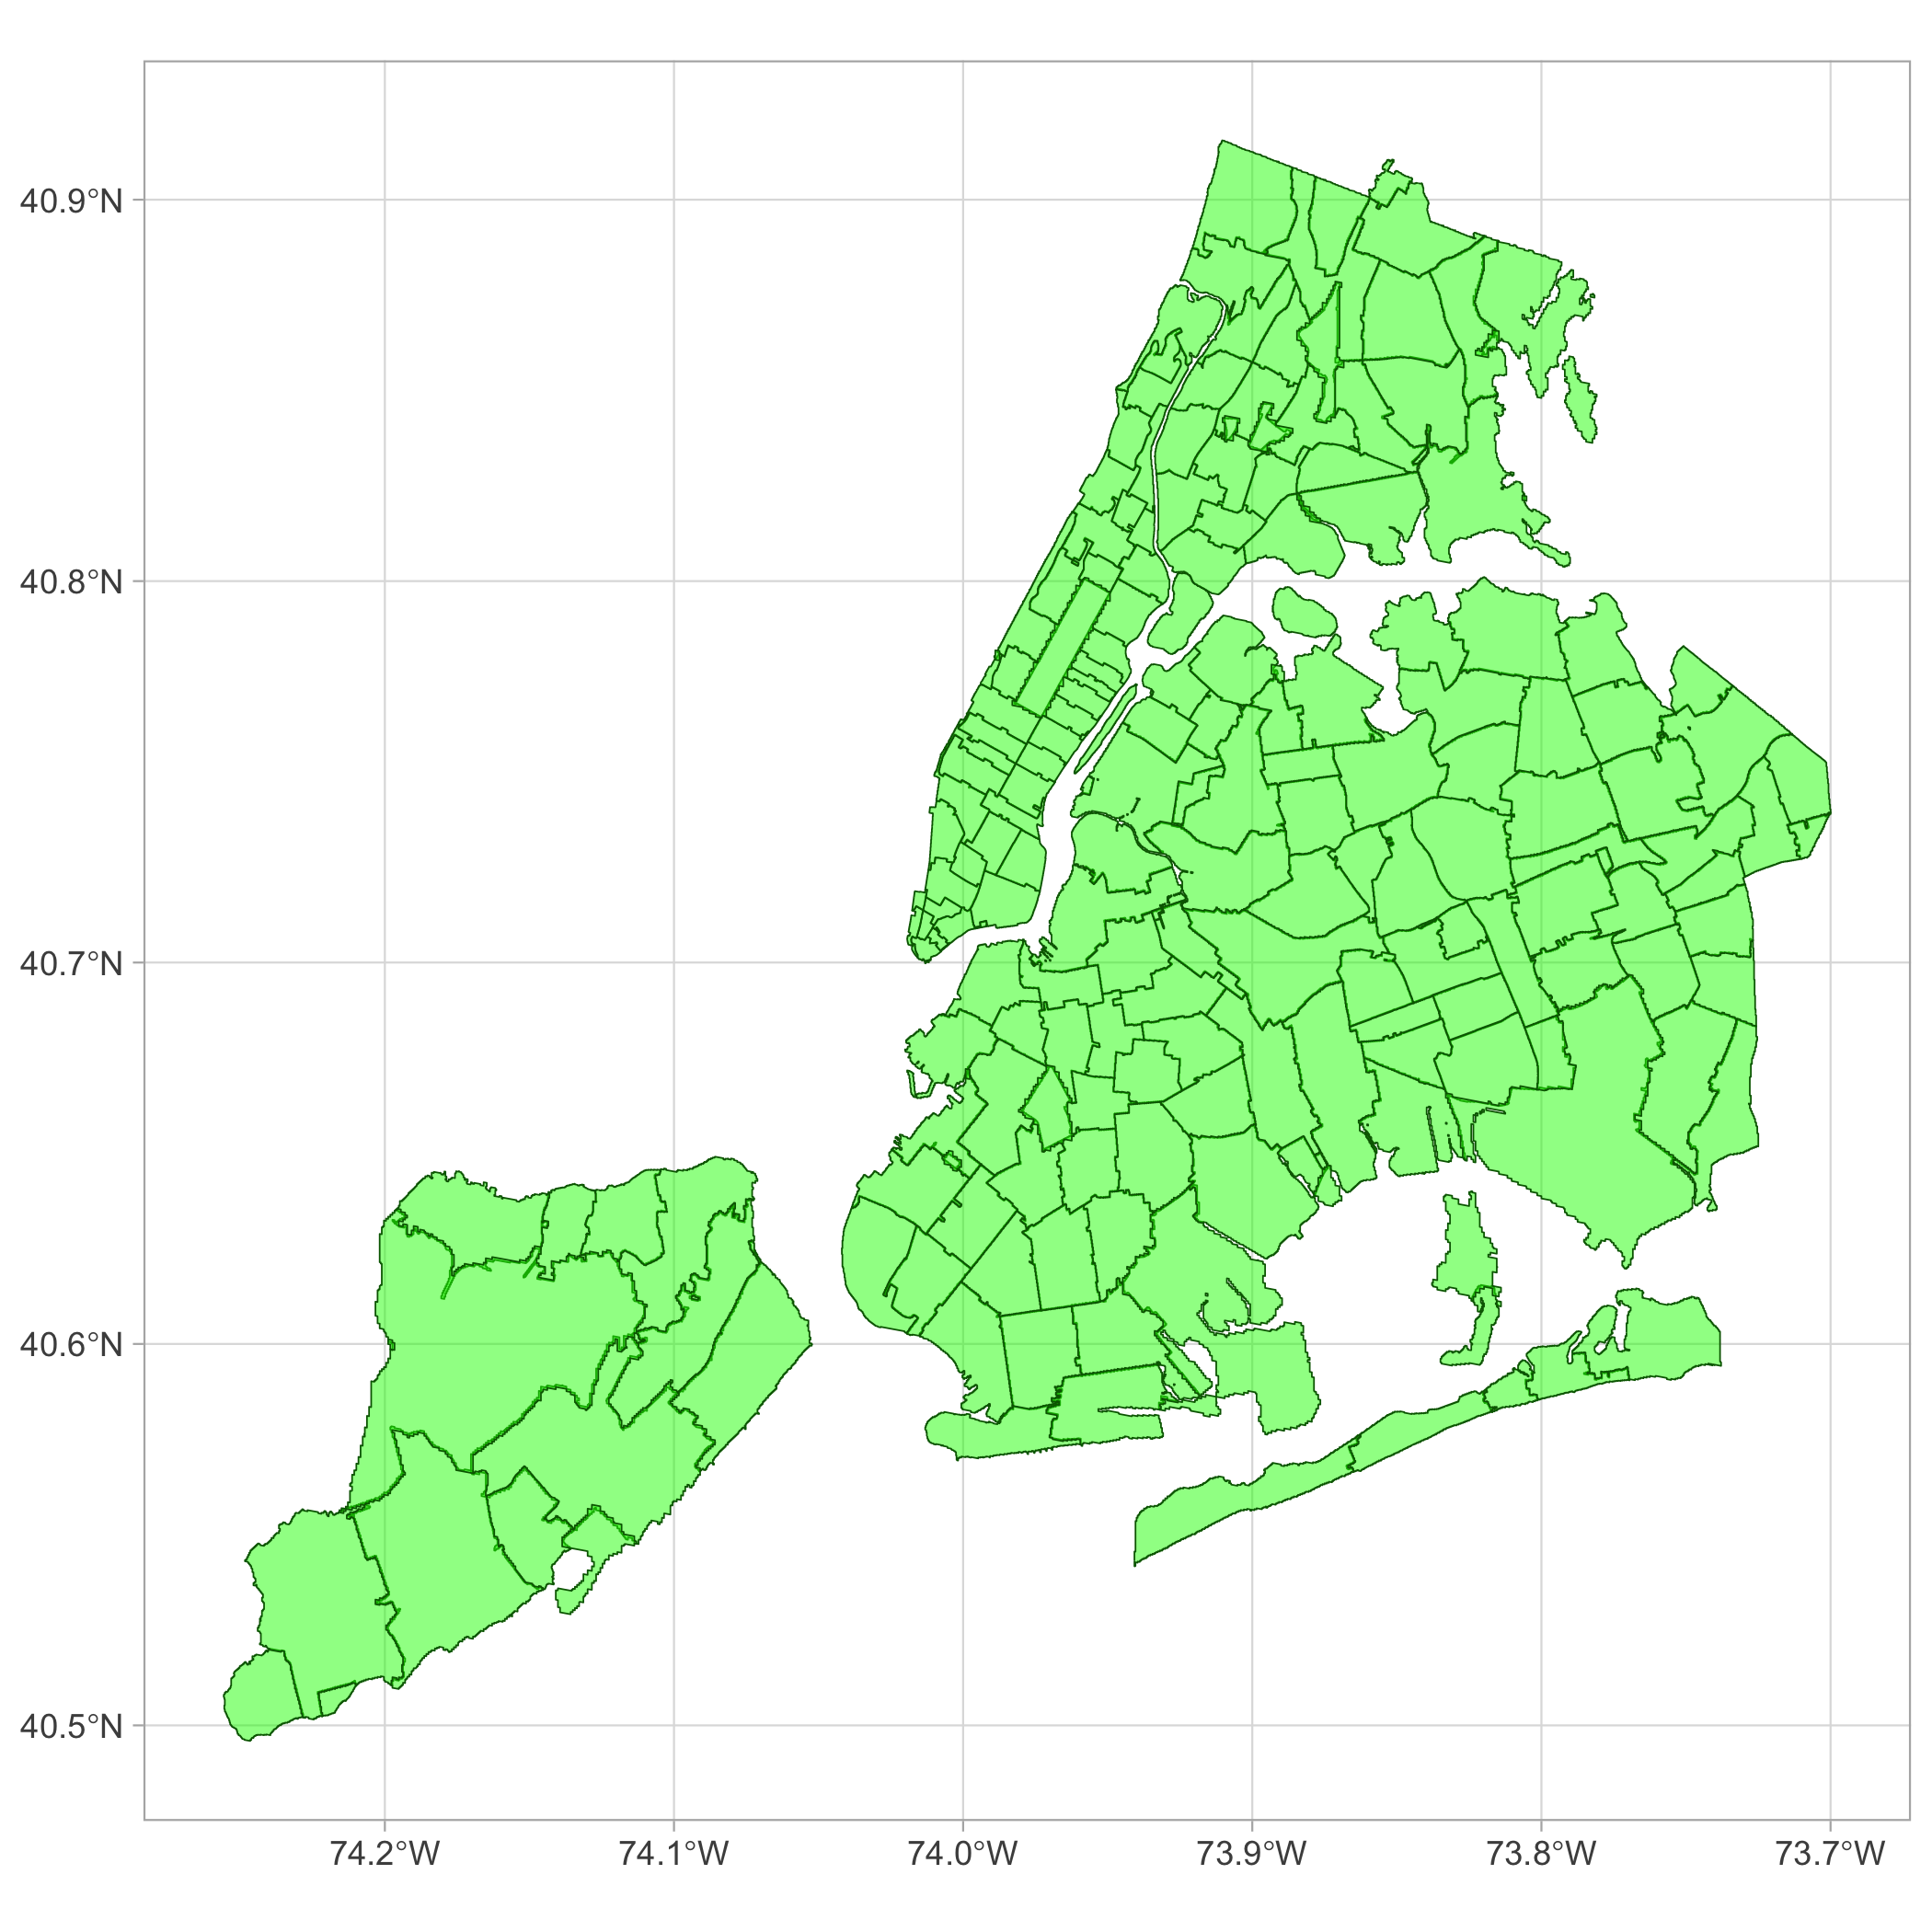
\includegraphics[width=0.3\linewidth]{out/eda/merged_gg.png}\label{merged}}
    \caption{NYC maps merged through spatial join show similarity to MODZCTA regions}
    \label{eda-map}
\end{figure*}

\subsubsection{Data Merging}
\begin{itemize}
    \item \textbf{COVID Data Integration}: The COVID data is joined by MODZCTA ID, ensuring that each region's case counts, case rates, death counts, and death rates are accurately represented.
    \item \textbf{Election Data Integration}: The election data is joined by electoral district ID. We filter the election data by year to focus on the 2020 and 2024 election results.
    \item \textbf{Merged Dataset}: The COVID data and election data are merged based on the geographic mapping, resulting in a comprehensive dataset that includes COVID metrics and election results for each region.
\end{itemize}

\subsubsection{Data Cleaning}
\begin{itemize}
    \item \textbf{Handling Missing Values}: For certain analyses, rows with missing values (NaN) are dropped to ensure the accuracy of the results.
    \item \textbf{Normalization}: The rates (case rates, death rates, vaccination rates) are normalized to floating-point numbers between 0 and 1. This allows for consistent representation of the data as percentages of the total population in each neighborhood.
\end{itemize}

This process ensures that the datasets are properly aligned and ready for subsequent analysis. By integrating and normalizing the data, we can accurately explore the relationships between political alignment and COVID-19 outcomes.

\subsection{Visualizing Distributions}

To understand the distribution of various metrics across NYC neighborhoods, we will create visualizations using histograms and maps.

\subsubsection{Histograms}
We will generate histograms to show the distributions of the following metrics:
\begin{itemize}
    \item \textbf{Case Rates per District}: The distribution of COVID-19 case rates across different electoral districts.
    \item \textbf{Death Rates per District}: The distribution of COVID-19 death rates across different electoral districts.
    \item \textbf{Vaccination Rates per District}: The distribution of COVID-19 vaccination rates across different electoral districts.
    \item \textbf{Proportion of Democratic Voters (2020/2024)}: The distribution of the proportion of votes for Democratic candidates in the 2020 and 2024 elections.
    \item \textbf{Proportion of Republican Voters (2020/2024)}: The distribution of the proportion of votes for Republican candidates in the 2020 and 2024 elections.
\end{itemize}

\subsubsection{Mapping Distributions}
We will also create maps to visualize the spatial distribution of these metrics:
\begin{itemize}
    \item \textbf{Density Maps}: Mapping the distributions allows us to see the density of the population for each targeted feature at a glance.
    \item \textbf{Overlaying Polygons}: For electoral districts, the overlaid polygons will accumulate results from separate electoral divisions, providing a comprehensive view of the data.
\end{itemize}

\subsection{Correlation Statistics}

To explore the relationships between COVID-19 metrics and election results, we will calculate and plot correlation statistics.

\subsubsection{Correlation Analysis}
We will analyze the correlations between the following pairs of metrics:
\begin{itemize}
    \item \textbf{COVID Case Rate vs. Voting Fraction (2020, 2024)}: Examining the relationship between the proportion of votes for Democratic and Republican candidates and the COVID-19 case rates in 2020 and 2024.
    \item \textbf{COVID Death Rate vs. Voting Fraction (2020, 2024)}: Investigating the correlation between the voting fractions and COVID-19 death rates in 2020 and 2024.
    \item \textbf{COVID Vaccination Rate vs. Voting Fraction (2020, 2024)}: Analyzing how vaccination rates correlate with the voting fractions in 2020 and 2024.
    \item \textbf{COVID Vaccination Rate vs. Case Rates}: Exploring the relationship between vaccination rates and COVID-19 case rates.
    \item \textbf{COVID Vaccination Rate vs. Death Rates}: Assessing the correlation between vaccination rates and COVID-19 death rates.
\end{itemize}

\subsubsection{Statistical Methods}
We will use the following statistical methods to calculate and visualize the correlations:
\begin{itemize}
    \item \textbf{Pearson Correlation Coefficient}: To measure the linear correlation between the pairs of metrics.
    \item \textbf{Scatter Plots}: To visualize the relationships between the pairs of metrics.
\end{itemize}

\subsection{Areal Statistics}

To account for spatial dependencies in the data, we will perform areal statistics analysis. This involves calculating spatial autocorrelation metrics and analyzing the spatial relationships between neighboring regions.

\subsubsection{Moran's I}
Moran's I is a measure of spatial autocorrelation, which indicates the degree to which a variable is similar to itself in nearby locations. We will calculate Moran's I using different spatial weights:
\begin{itemize}
    \item \textbf{6 Nearest Neighbors (6NN)}: Considering the six closest neighboring regions for each area.
    \item \textbf{Queen Contiguity}: Considering regions that share a common boundary or vertex.
    \item \textbf{Inverse Distance Weighting (IDW)}: Considering the influence of neighboring regions based on the inverse of their distance.
\end{itemize}

\subsubsection{Correlograms}
Correlograms will be generated to visualize the autocorrelative effects across neighboring regions. These plots will help us understand how the spatial relationships between regions influence the distribution of COVID-19 metrics and political alignment.

\subsubsection{Other areal analysis}
We will also perform the following additional analyses:

\begin{itemize}
    \item \textbf{Getis-Ord Gi* Statistic}: The Getis-Ord Gi* statistic identifies clusters of high or low values, detecting hotspots and cold spots within the dataset.
    \item \textbf{Spatial Autoregressive (SAR) Model}: The SAR model accounts for spatial dependencies by incorporating spatial lag-errors, analyzing the influence of neighboring regions on COVID-19 case rates, vaccination rates, and political alignment.
    \item \textbf{Conditional Autoregressive (CAR) Model}: The CAR model considers the conditional distribution of each region given its neighbors, helping to understand the influence of the spatial structure on COVID-19 case rates, vaccination rates, and political alignment.
\end{itemize}

\subsection{Code}

All code and analyses is available in a public repository at \url{https://github.com/john-s-lin/vax-populi}.

\section{Results}

\subsection{Distributions and Maps of COVID Case Rates, Death Rates, and Vaccinations}

\subsubsection{Case Rates}

The analysis of COVID-19 case rates across New York City reveals significant insights into the spread of the virus in different neighborhoods. For one, the average case rate per district is approximately 0.4 (Fig. \ref{hist-case}), indicating that, on average, 2 out of 5 people in NYC have had COVID-19 at some point contracted COVID-19. Additionally, the case counts did not exceed 50,000 cases per 100,000 people, resulting in a maximum case rate of 0.5.

The map (Fig. \ref{map-case}) also shows several hotspots:
\begin{itemize}
    \item \textbf{Staten Island}: Significant hotspots are observed in Staten Island.
    \item \textbf{Midtown Manhattan}: A hotspot is identified in Midtown Manhattan, an area known for its high density due to tourist attractions.
    \item \textbf{Rockaway Beach}: Another hotspot is located in Rockaway Beach at the southern border of Queens.
\end{itemize}

\begin{figure*}[t]
    \centering
    \subfloat[Histogram]{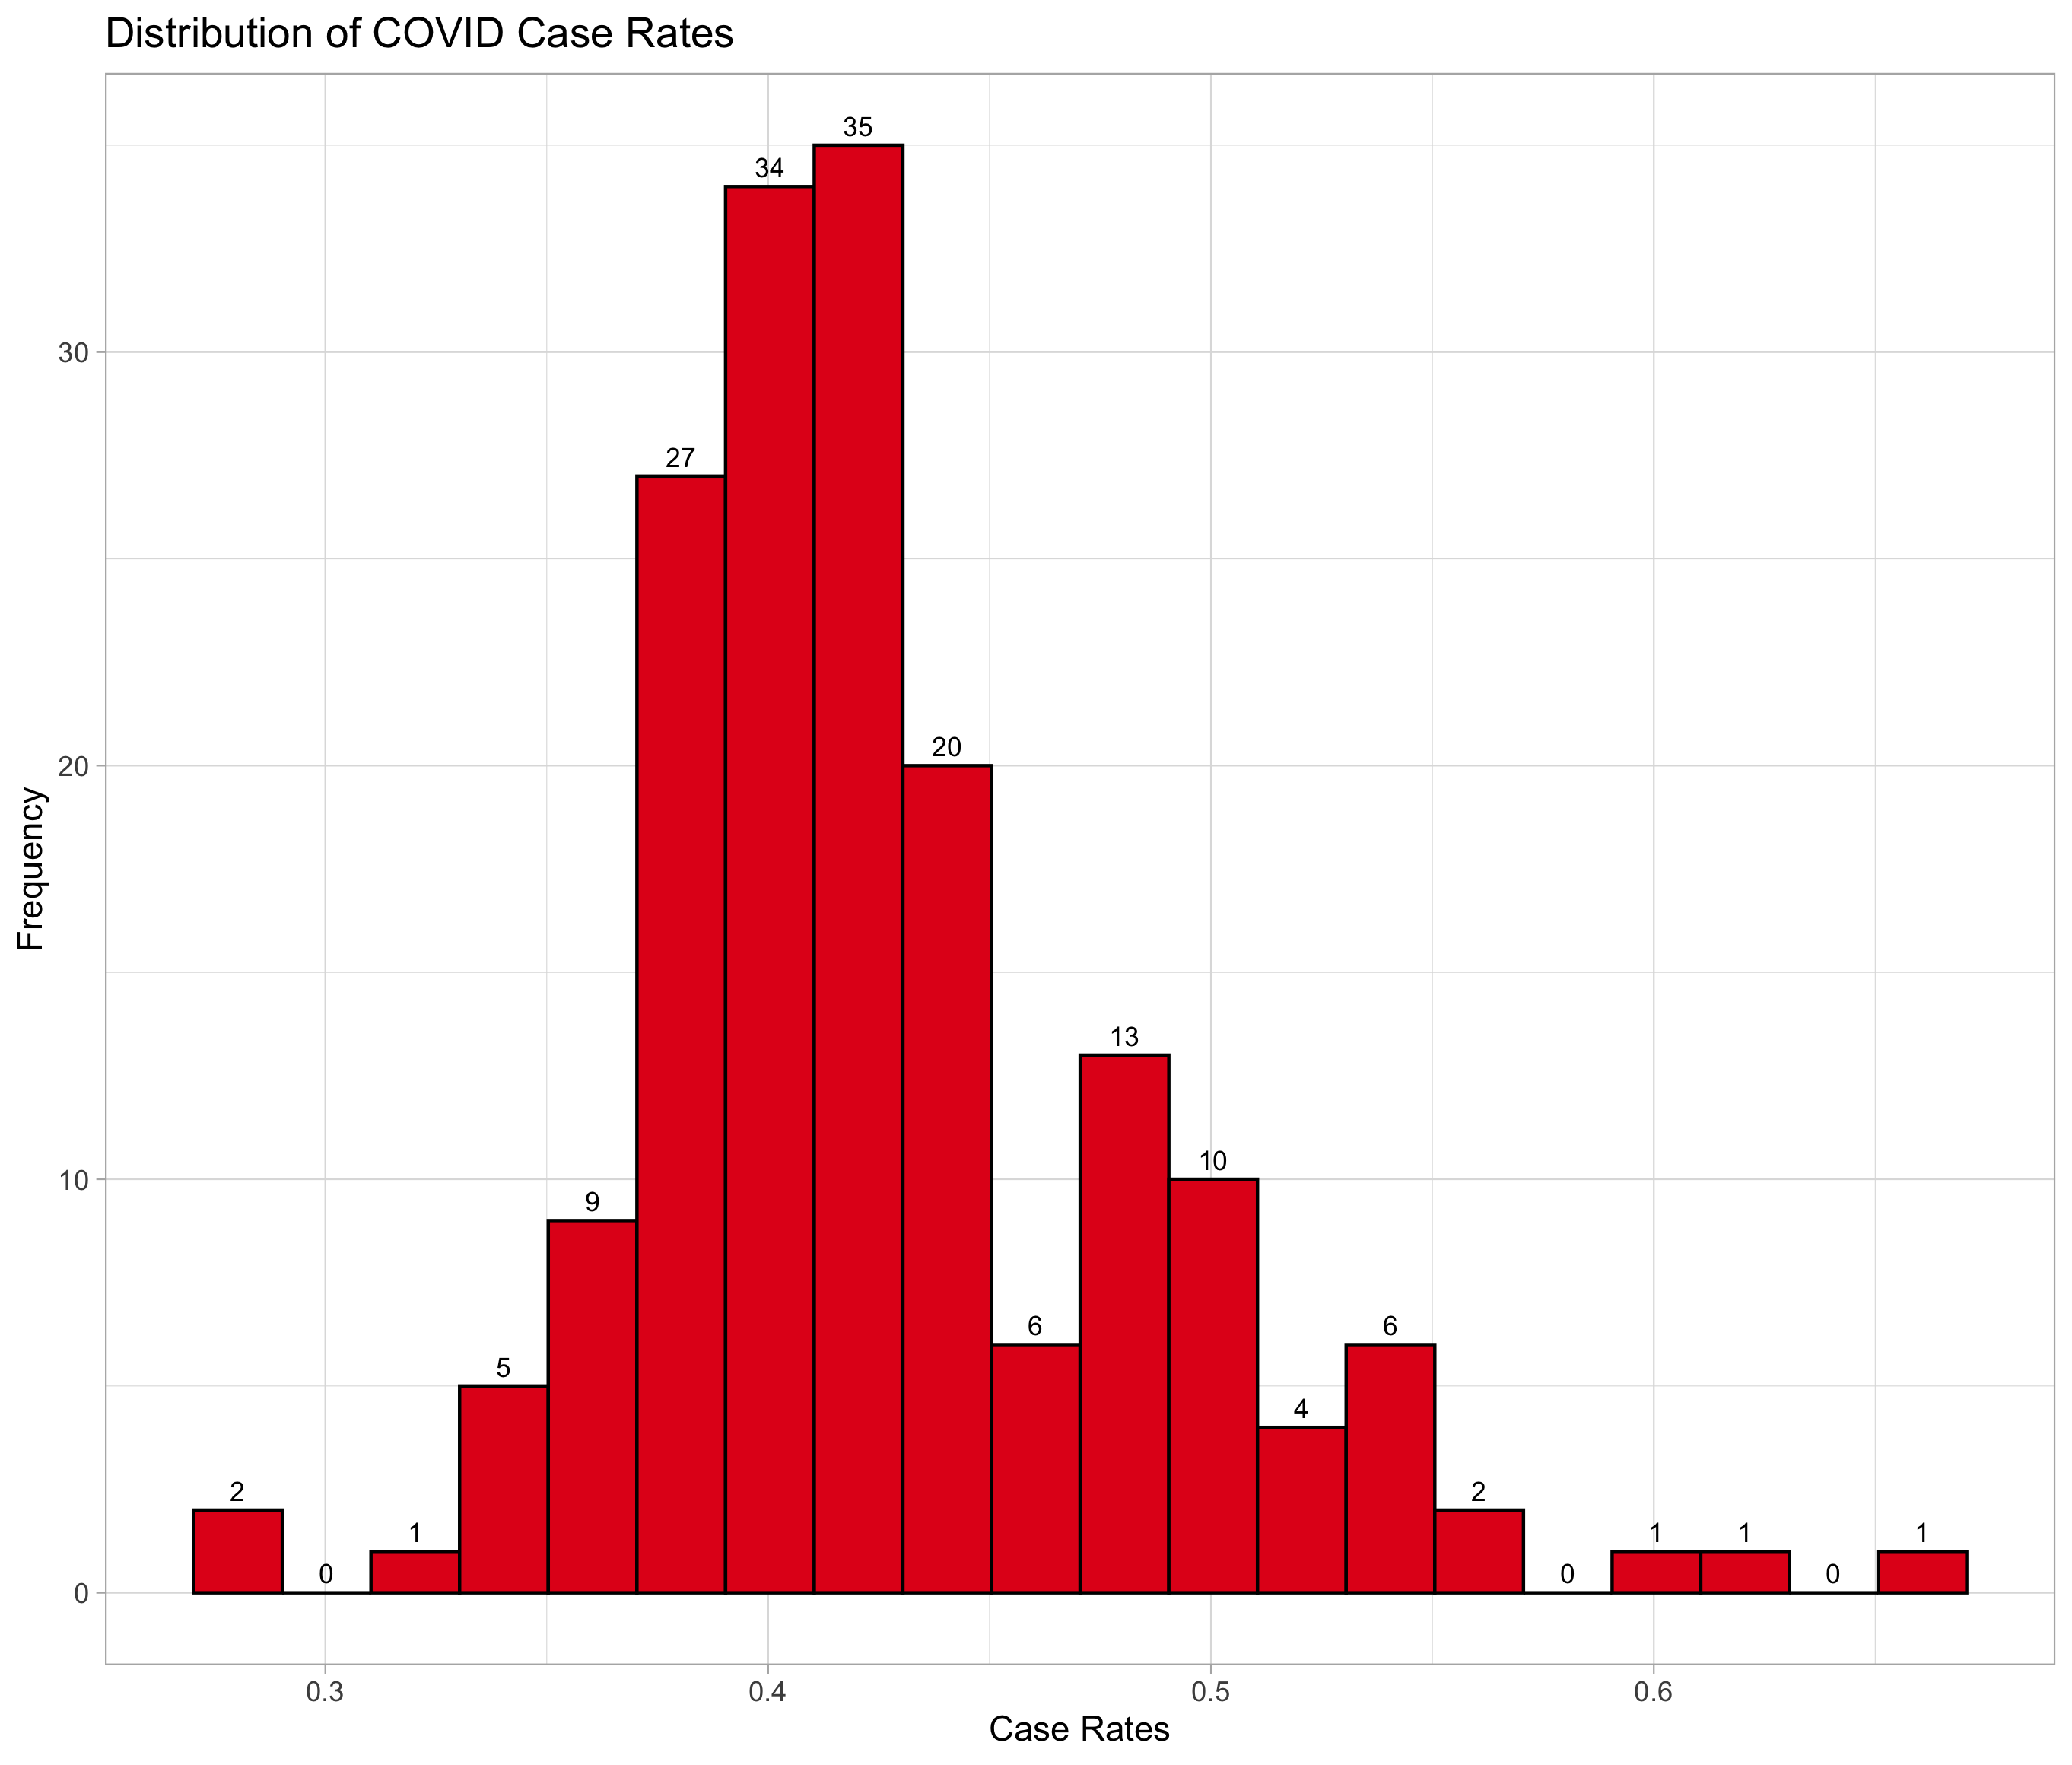
\includegraphics[width=0.5\linewidth]{out/histograms/covid_case_rates_hist.png}\label{hist-case}}
    \subfloat[Map]{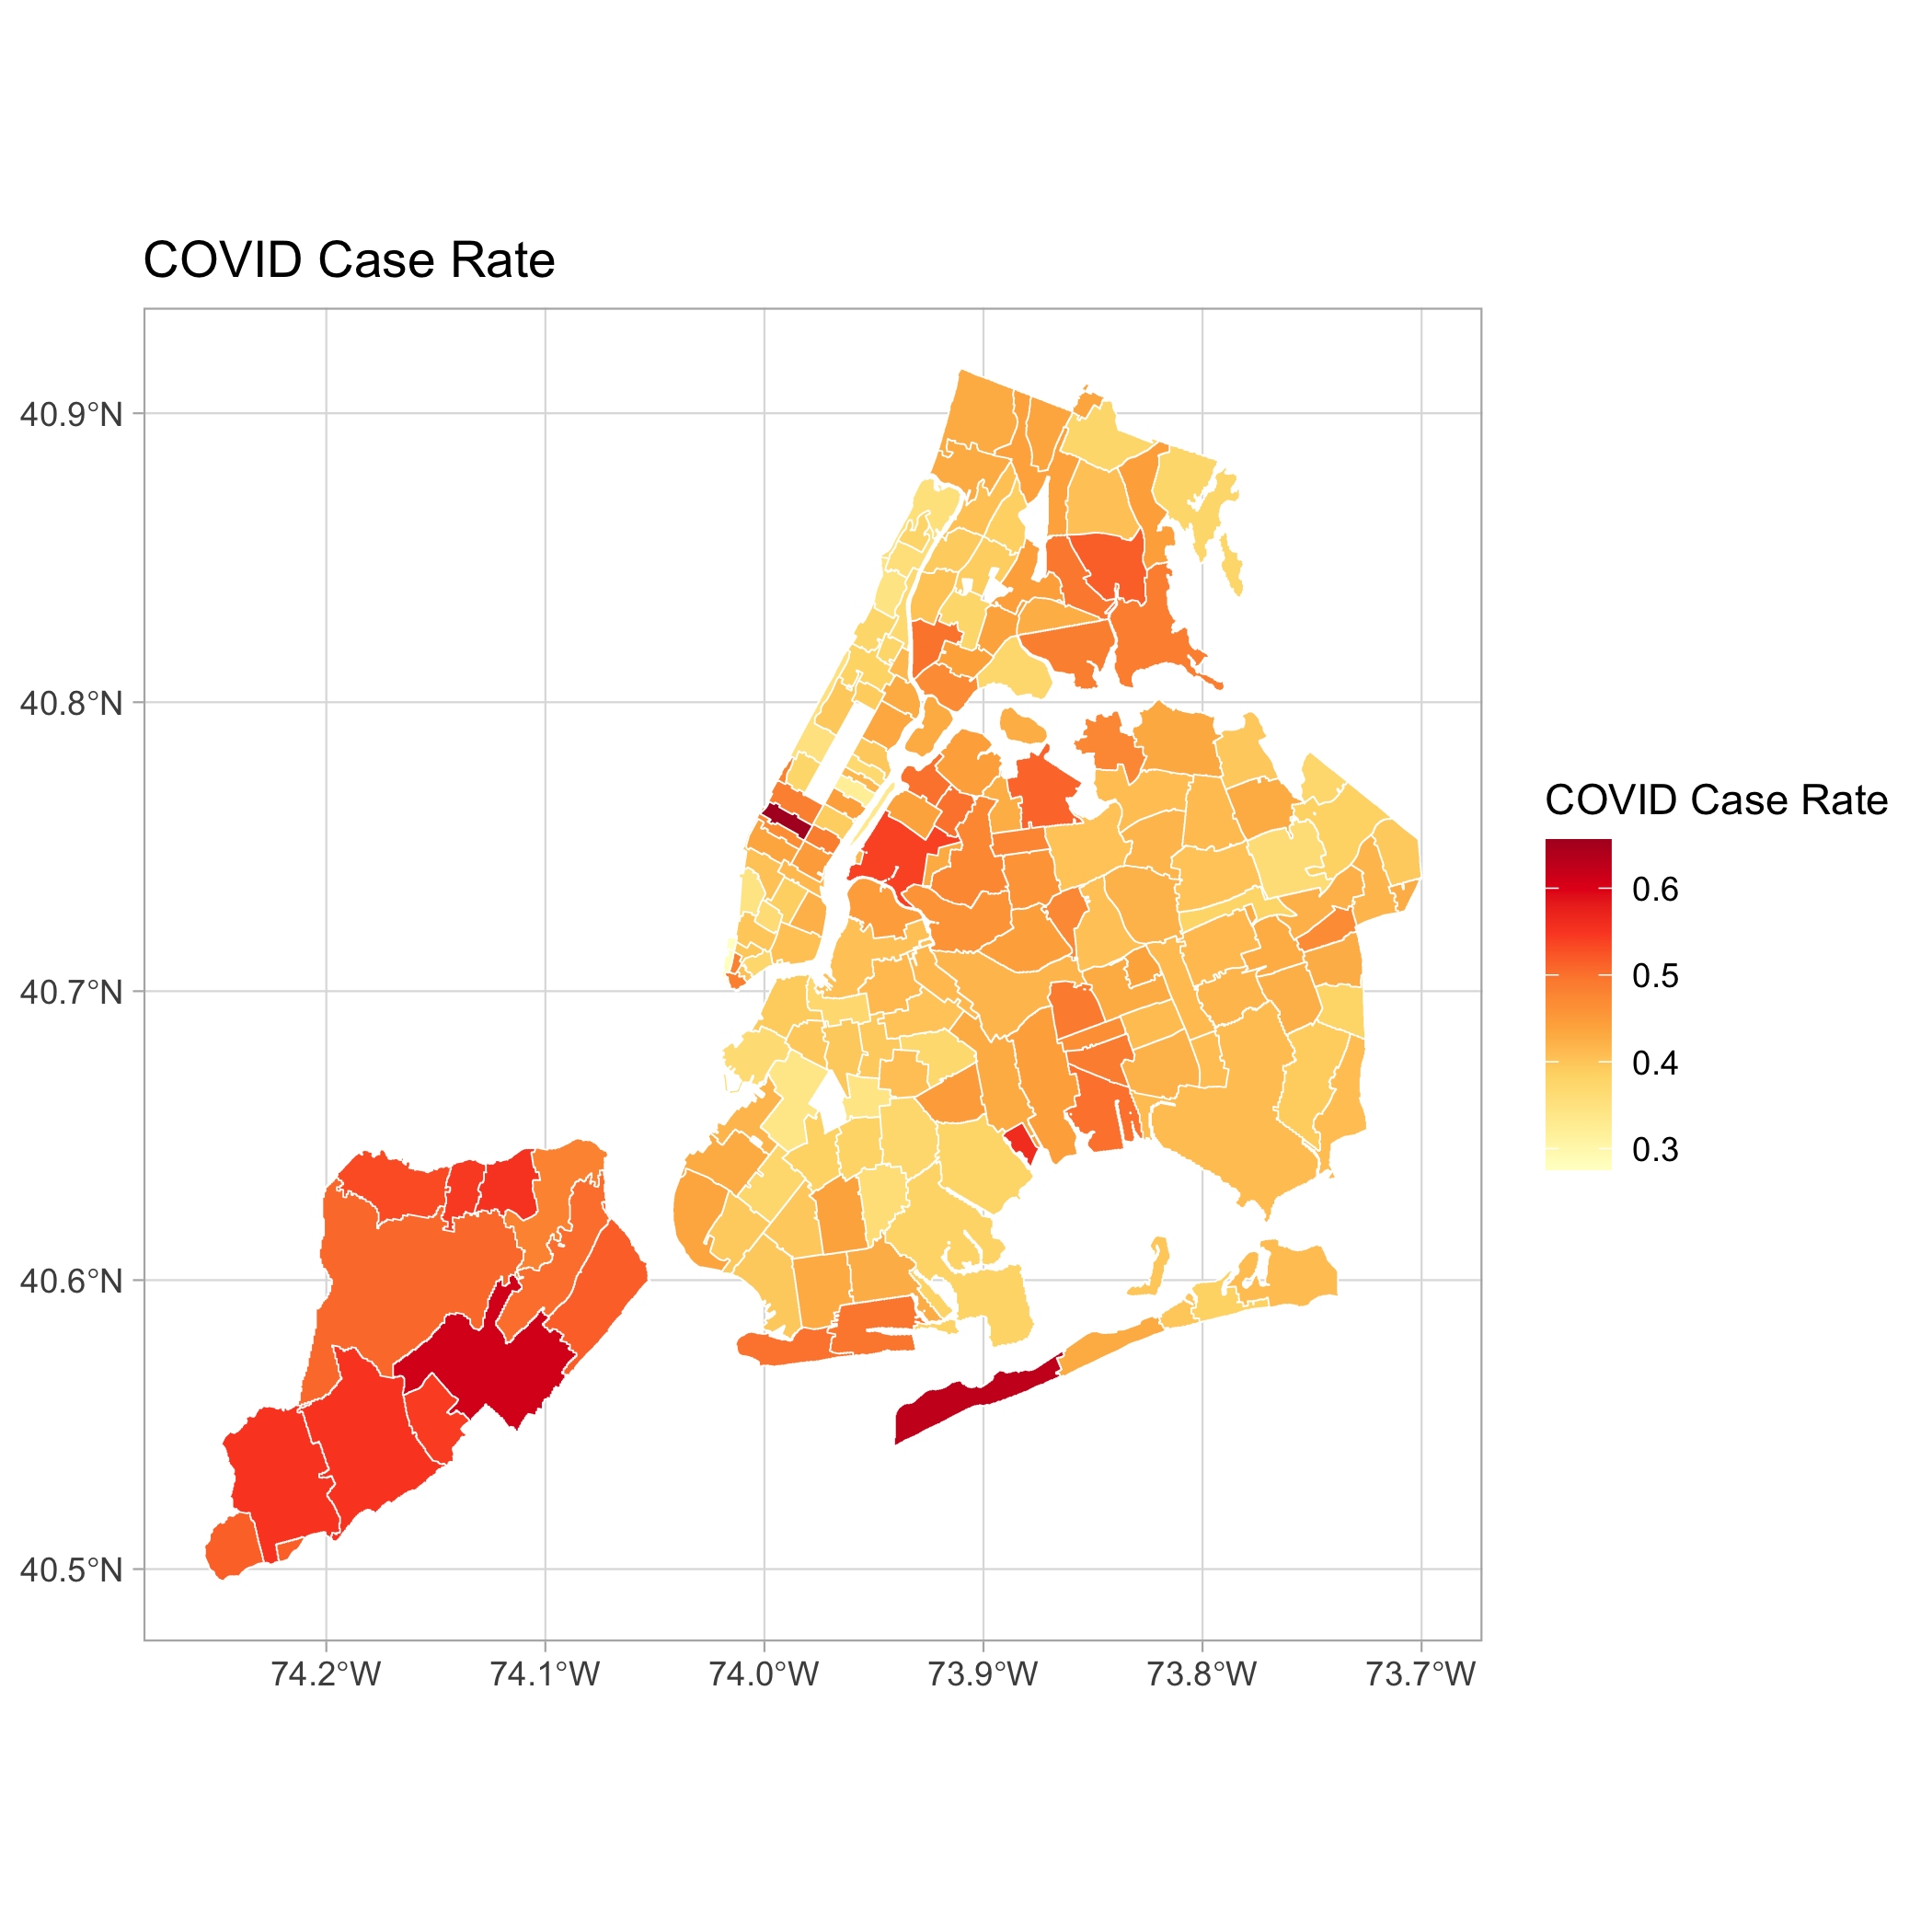
\includegraphics[width=0.425\linewidth]{out/maps/covid_case_rate_map_gg.png}\label{map-case}}
    \caption{NYC COVID Case Rates}
\end{figure*}

\subsubsection{Death Rates}

The analysis of COVID-19 death rates across New York City provides insights into the mortality impact of the virus in different neighborhoods.

\begin{itemize}
    \item \textbf{Average Death Rate}: The average death rate per district is approximately 0.5\%, indicating that the mortality rate due to COVID-19 was relatively low across NYC (Fig. \ref{hist-death}).
    \item \textbf{Spatial Distribution}: The death rate is relatively evenly spread across all districts, with a few exceptions (Fig. \ref{map-death}):
    \begin{itemize}
        \item \textbf{Southern Brooklyn}: Isolated districts in southern Brooklyn show slightly higher death rates.
        \item \textbf{Queens}: Similar isolated districts in Queens also exhibit higher death rates.
    \end{itemize}
\end{itemize}

\begin{figure*}[t]
    \centering
    \subfloat[Histogram]{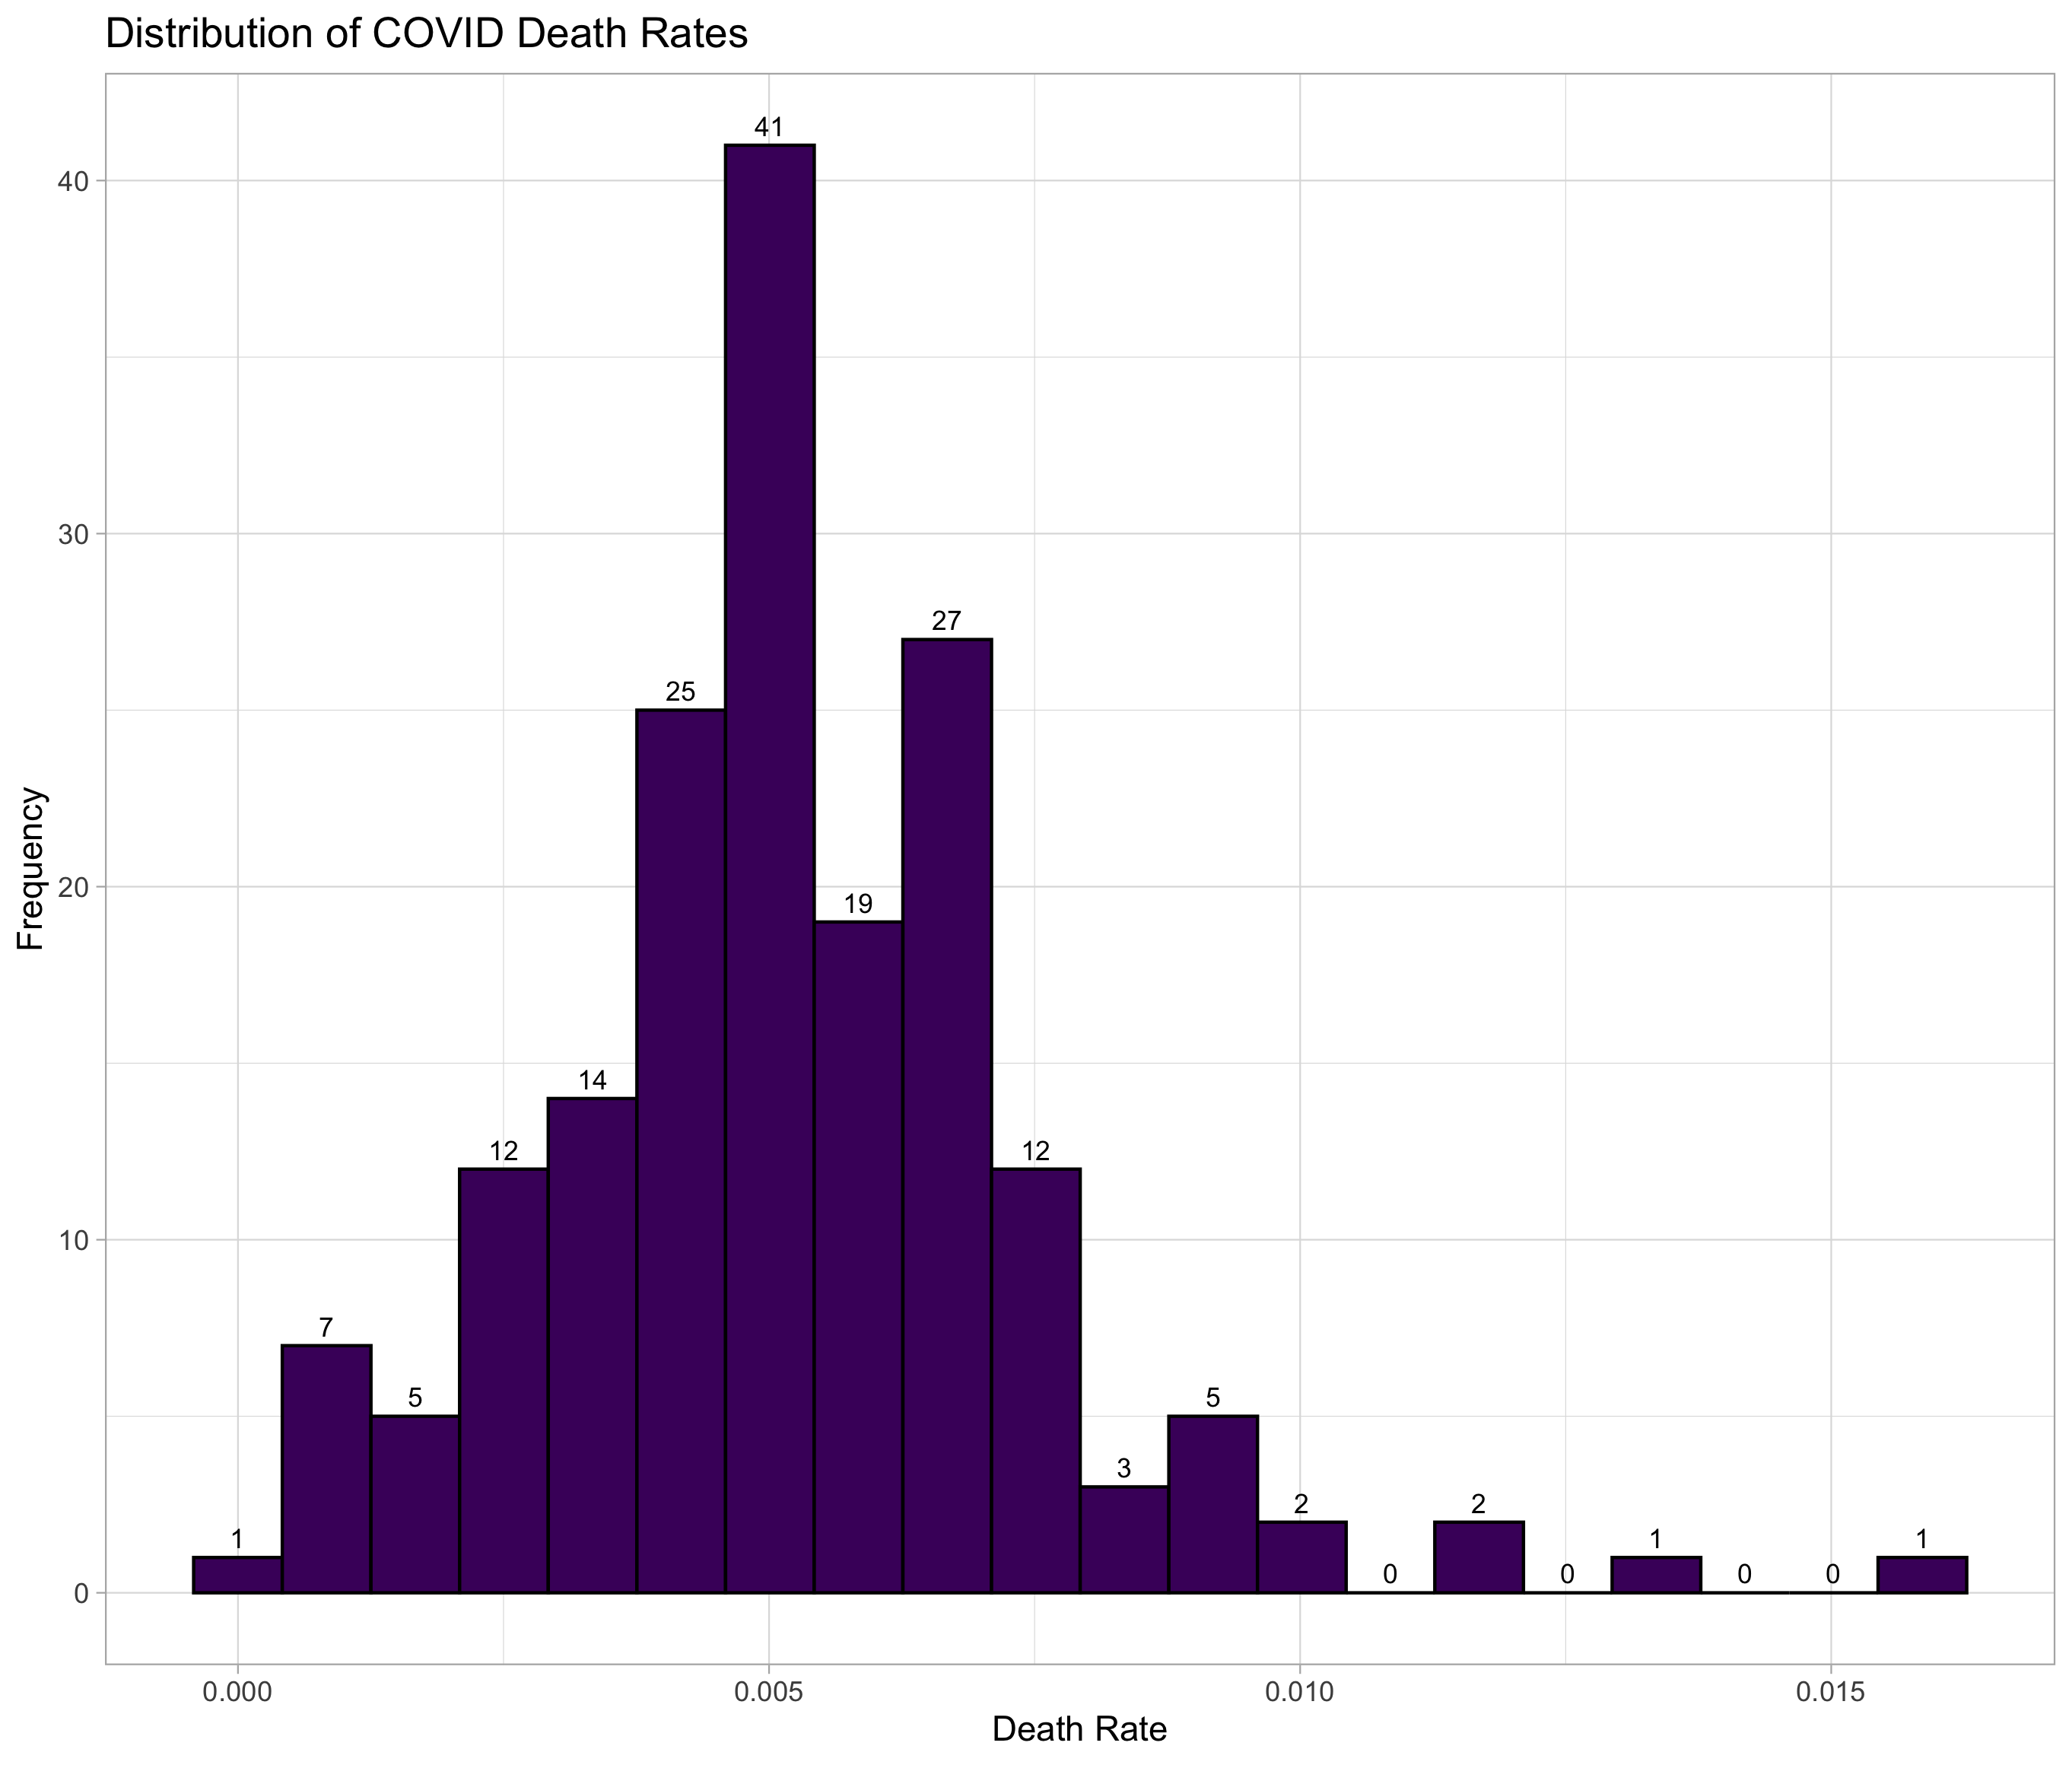
\includegraphics[width=0.5\linewidth]{out/histograms/covid_death_rates_hist.png}\label{hist-death}}
    \subfloat[Map]{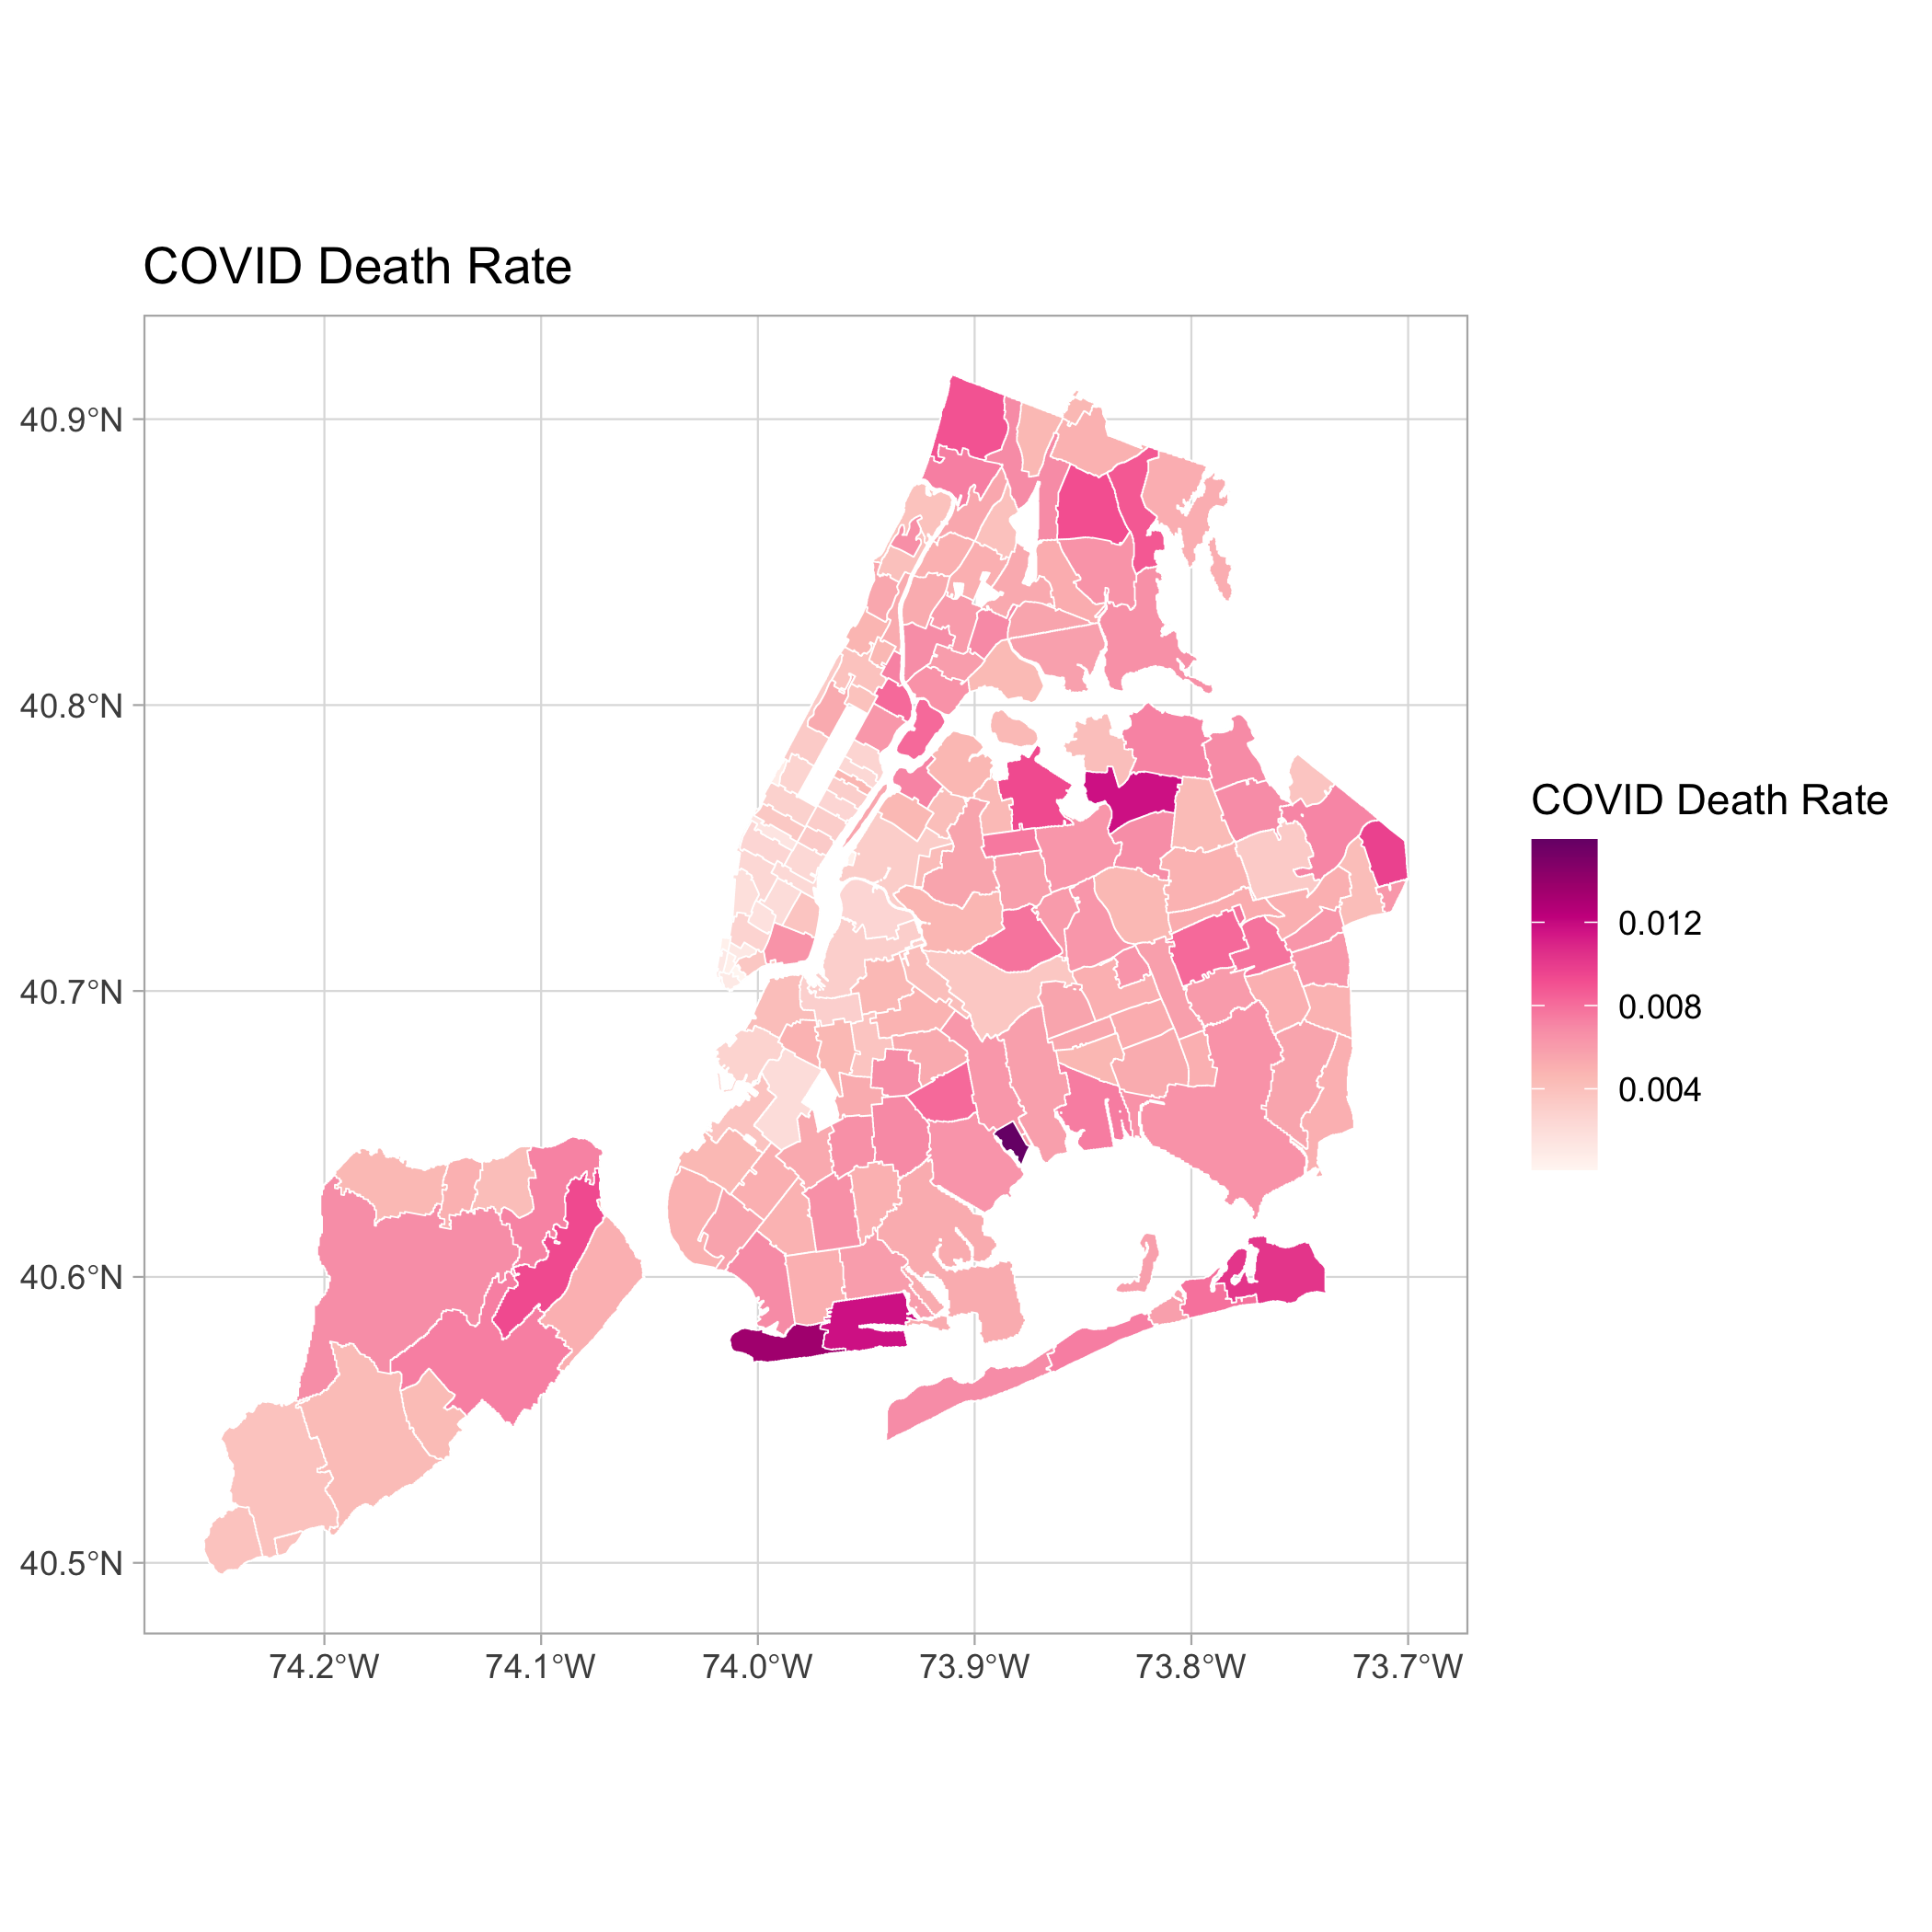
\includegraphics[width=0.425\linewidth]{out/maps/covid_death_rate_map_gg.png}\label{map-death}}
    \caption{NYC COVID Death Rates}
\end{figure*}

\subsubsection{Vaccination Rates}

The analysis of COVID-19 vaccination rates across New York City provides insights into the uptake of vaccines in different neighborhoods.

\begin{itemize}
    \item \textbf{High Vaccination Rates}: The percentage of fully vaccinated individuals in each district is very high, with many districts having vaccination rates greater than 2 doses per person, indicating booster vaccinations (Fig. \ref{hist-vax}).
    \item \textbf{Average Vaccination Rate}: The average vaccination rate across districts is approximately 0.9. This high average suggests that a significant portion of the population received full vaccination, including booster doses.
    \item \textbf{Spatial Distribution}: The vaccination rates are relatively high across most districts, with some variation (Fig. \ref{map-vax}):
    \begin{itemize}
        \item \textbf{Higher Rates}: Many districts have vaccination rates above 1, indicating that a substantial number of individuals received more than the initial two doses.
        \item \textbf{Variation}: While the overall vaccination rates are high, there are variations across different neighborhoods, reflecting differences in vaccine uptake.
    \end{itemize}
\end{itemize}

\begin{figure*}[t]
    \centering
    \subfloat[Histogram]{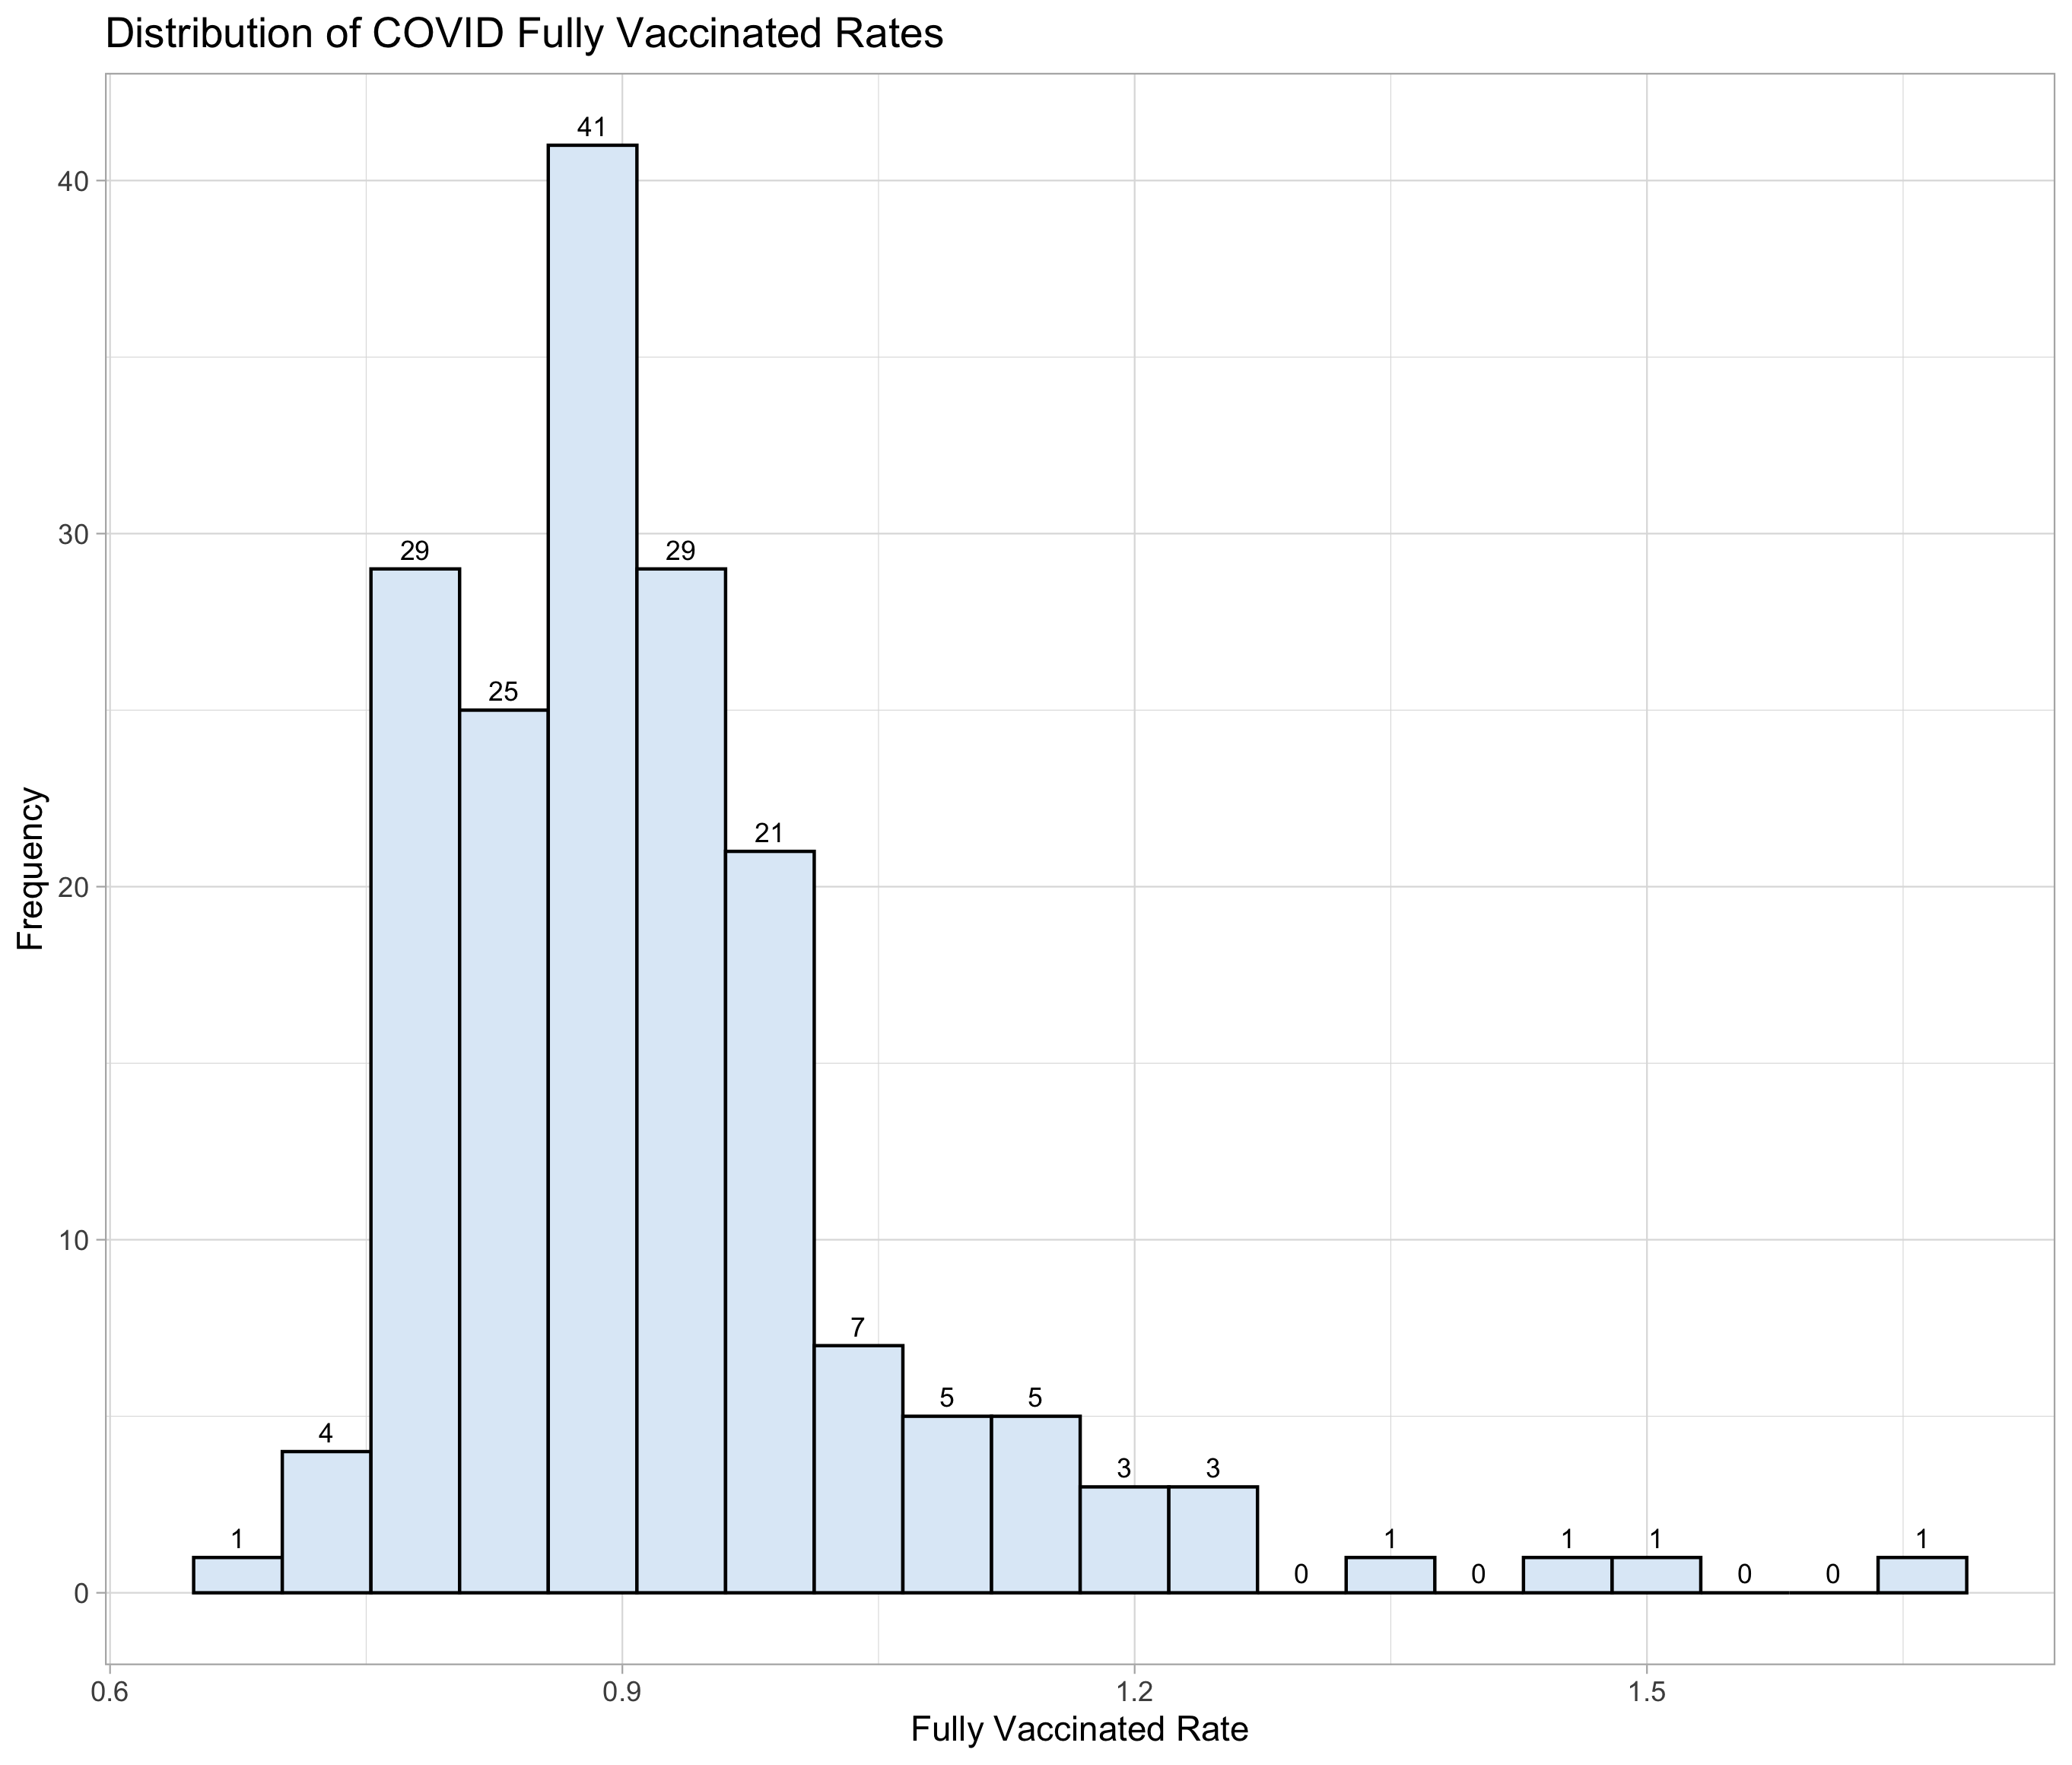
\includegraphics[width=0.5\linewidth]{out/histograms/covid_vax_rate_hist.png}\label{hist-vax}}
    \subfloat[Map]{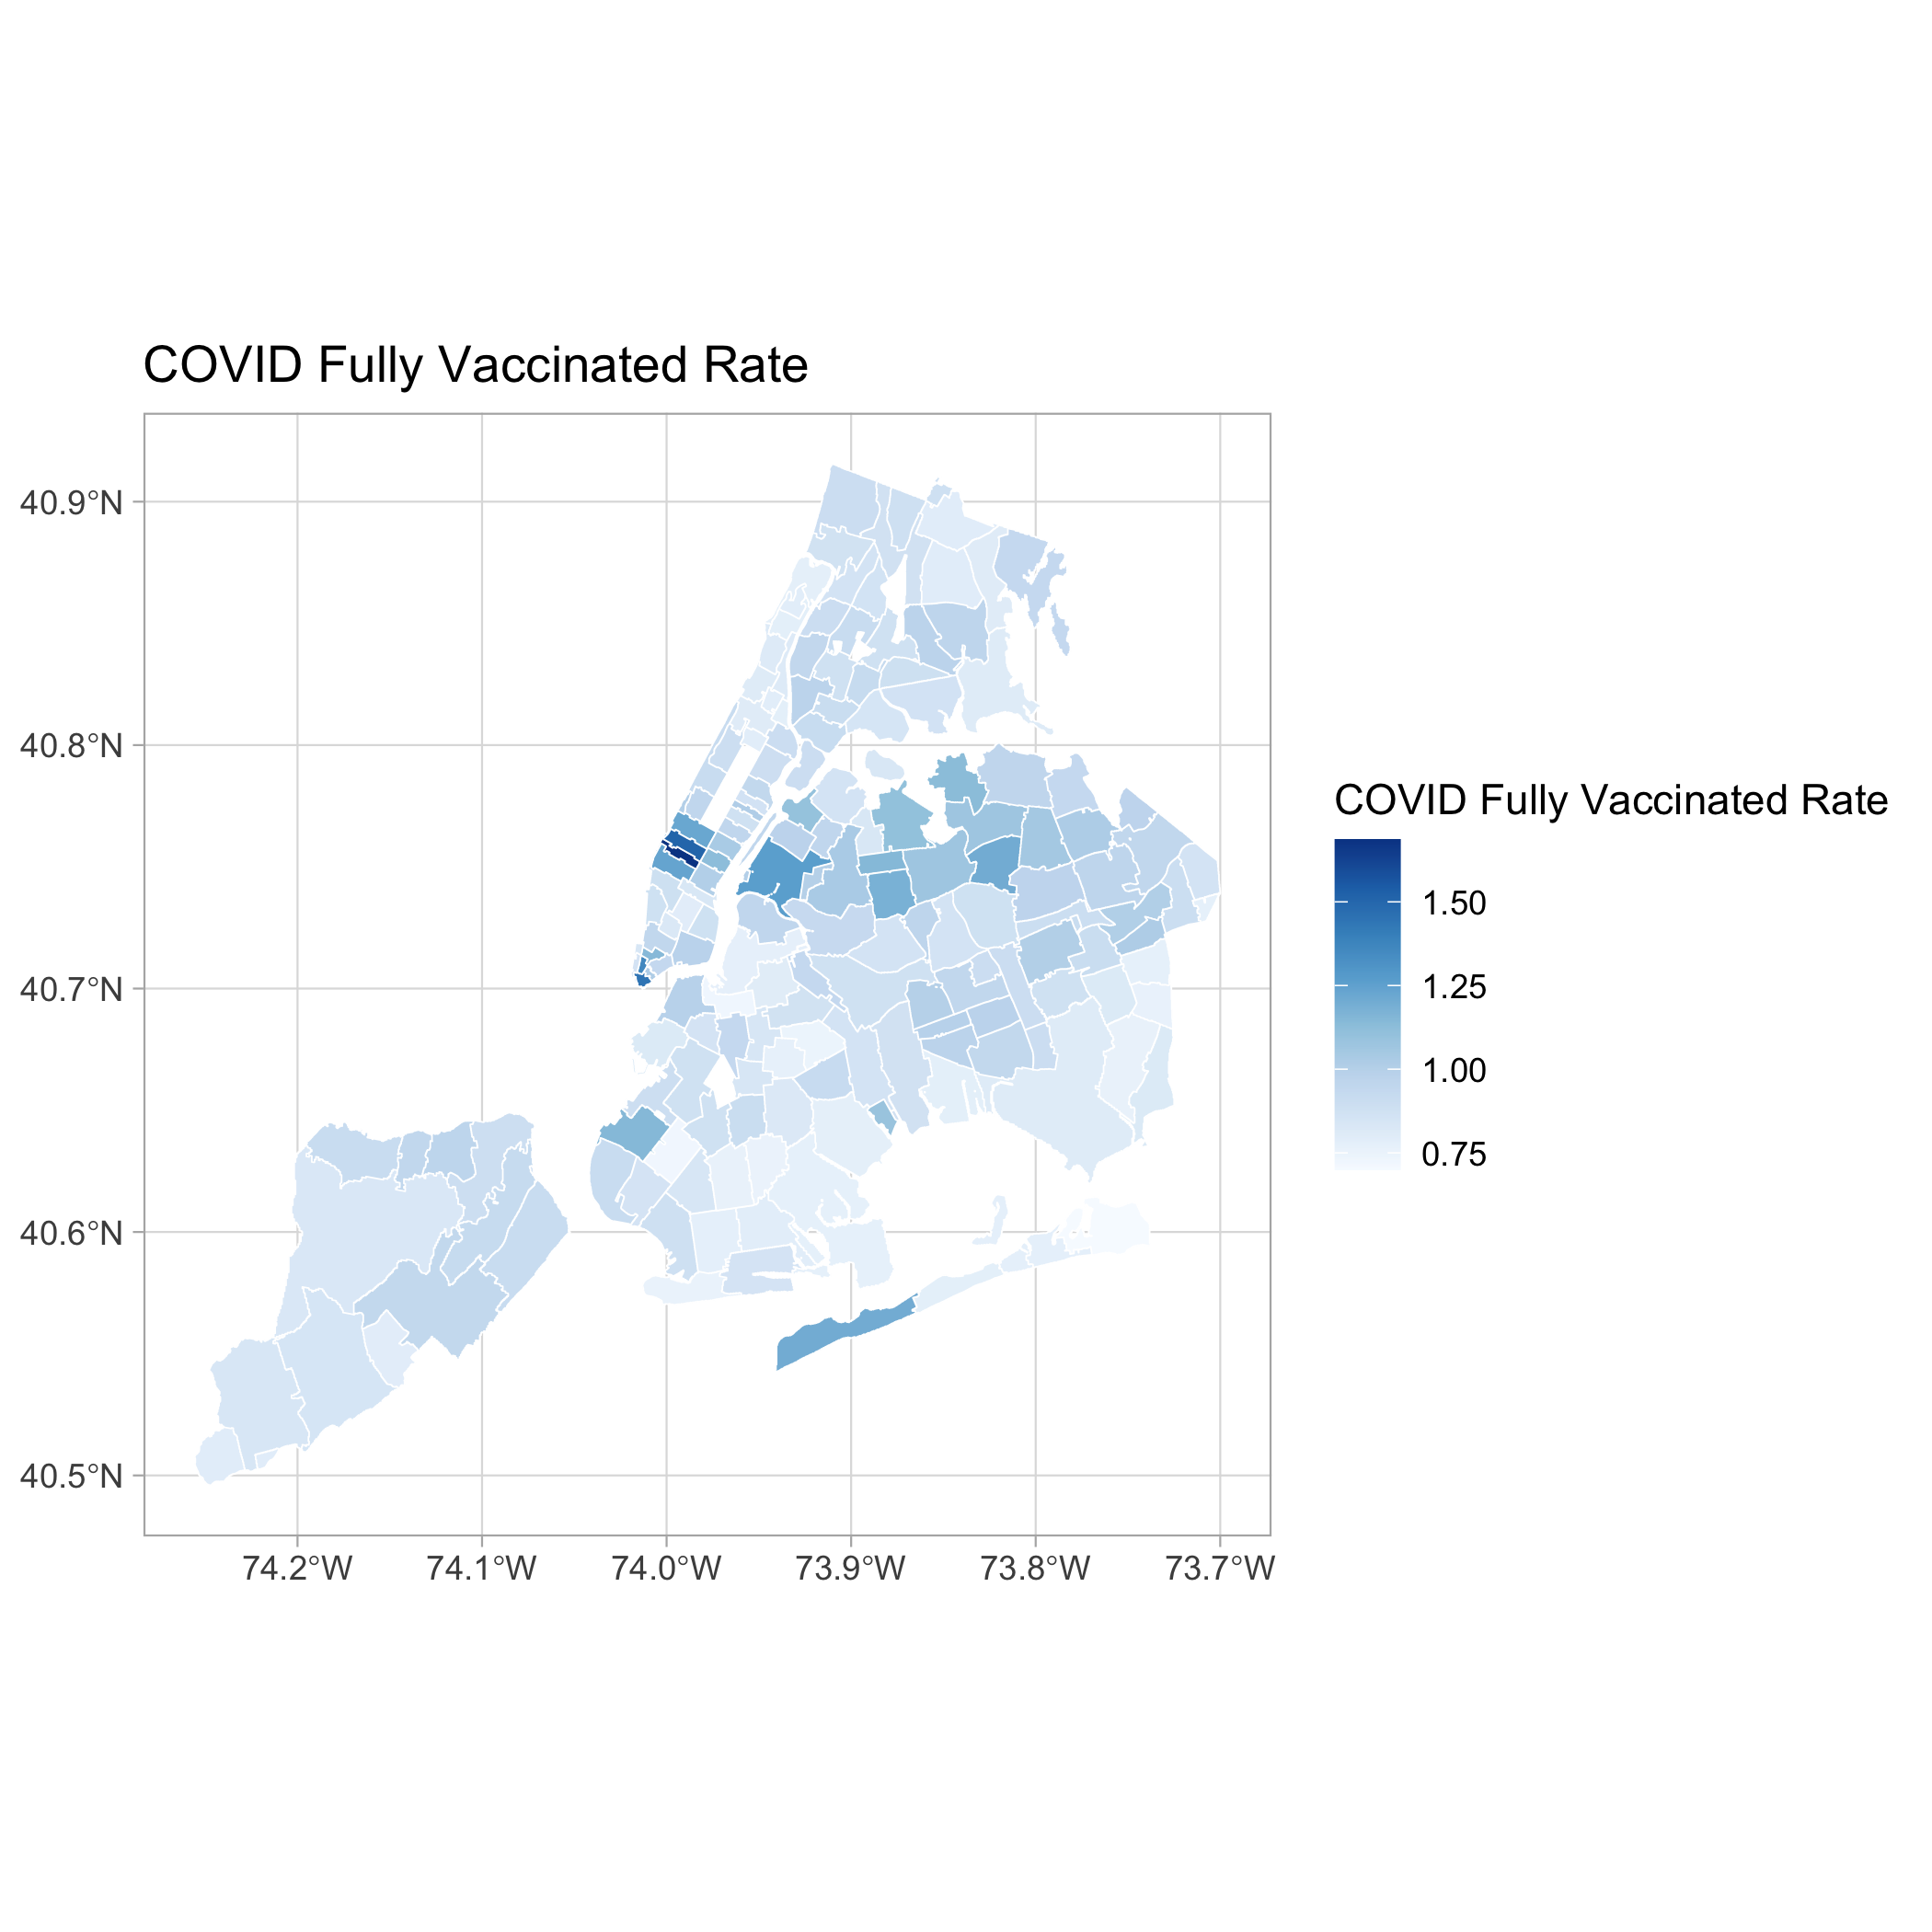
\includegraphics[width=0.425\linewidth]{out/maps/covid_vax_rate_map_gg.png}\label{map-vax}}
    \caption{NYC COVID Full Vaccination Rates}
\end{figure*}

\subsection{Distributions of Election Results}

\subsubsection{2020}
For the most part, NYC was predominantly left-leaning in 2020, with many districts showing a higher Democrat-Republican voting ratio. However, Staten Island and southern Brooklyn had more communities voting significantly to the right (Fig. \ref{ed-2020}).

\subsubsection{2024}
In 2024, NYC shifted more towards the right, with more districts in northern Queens becoming conservative. The ratio of Democrat to Republican voters decreased, with Staten Island, southern, and central Brooklyn becoming more conservative, while Manhattan, Queens, and the Bronx still had a higher Democrat voting ratio but showed a shift towards conservatism (Fig. \ref{ed-2024}).

\begin{figure*}[t]
    \centering
    \subfloat[2020]{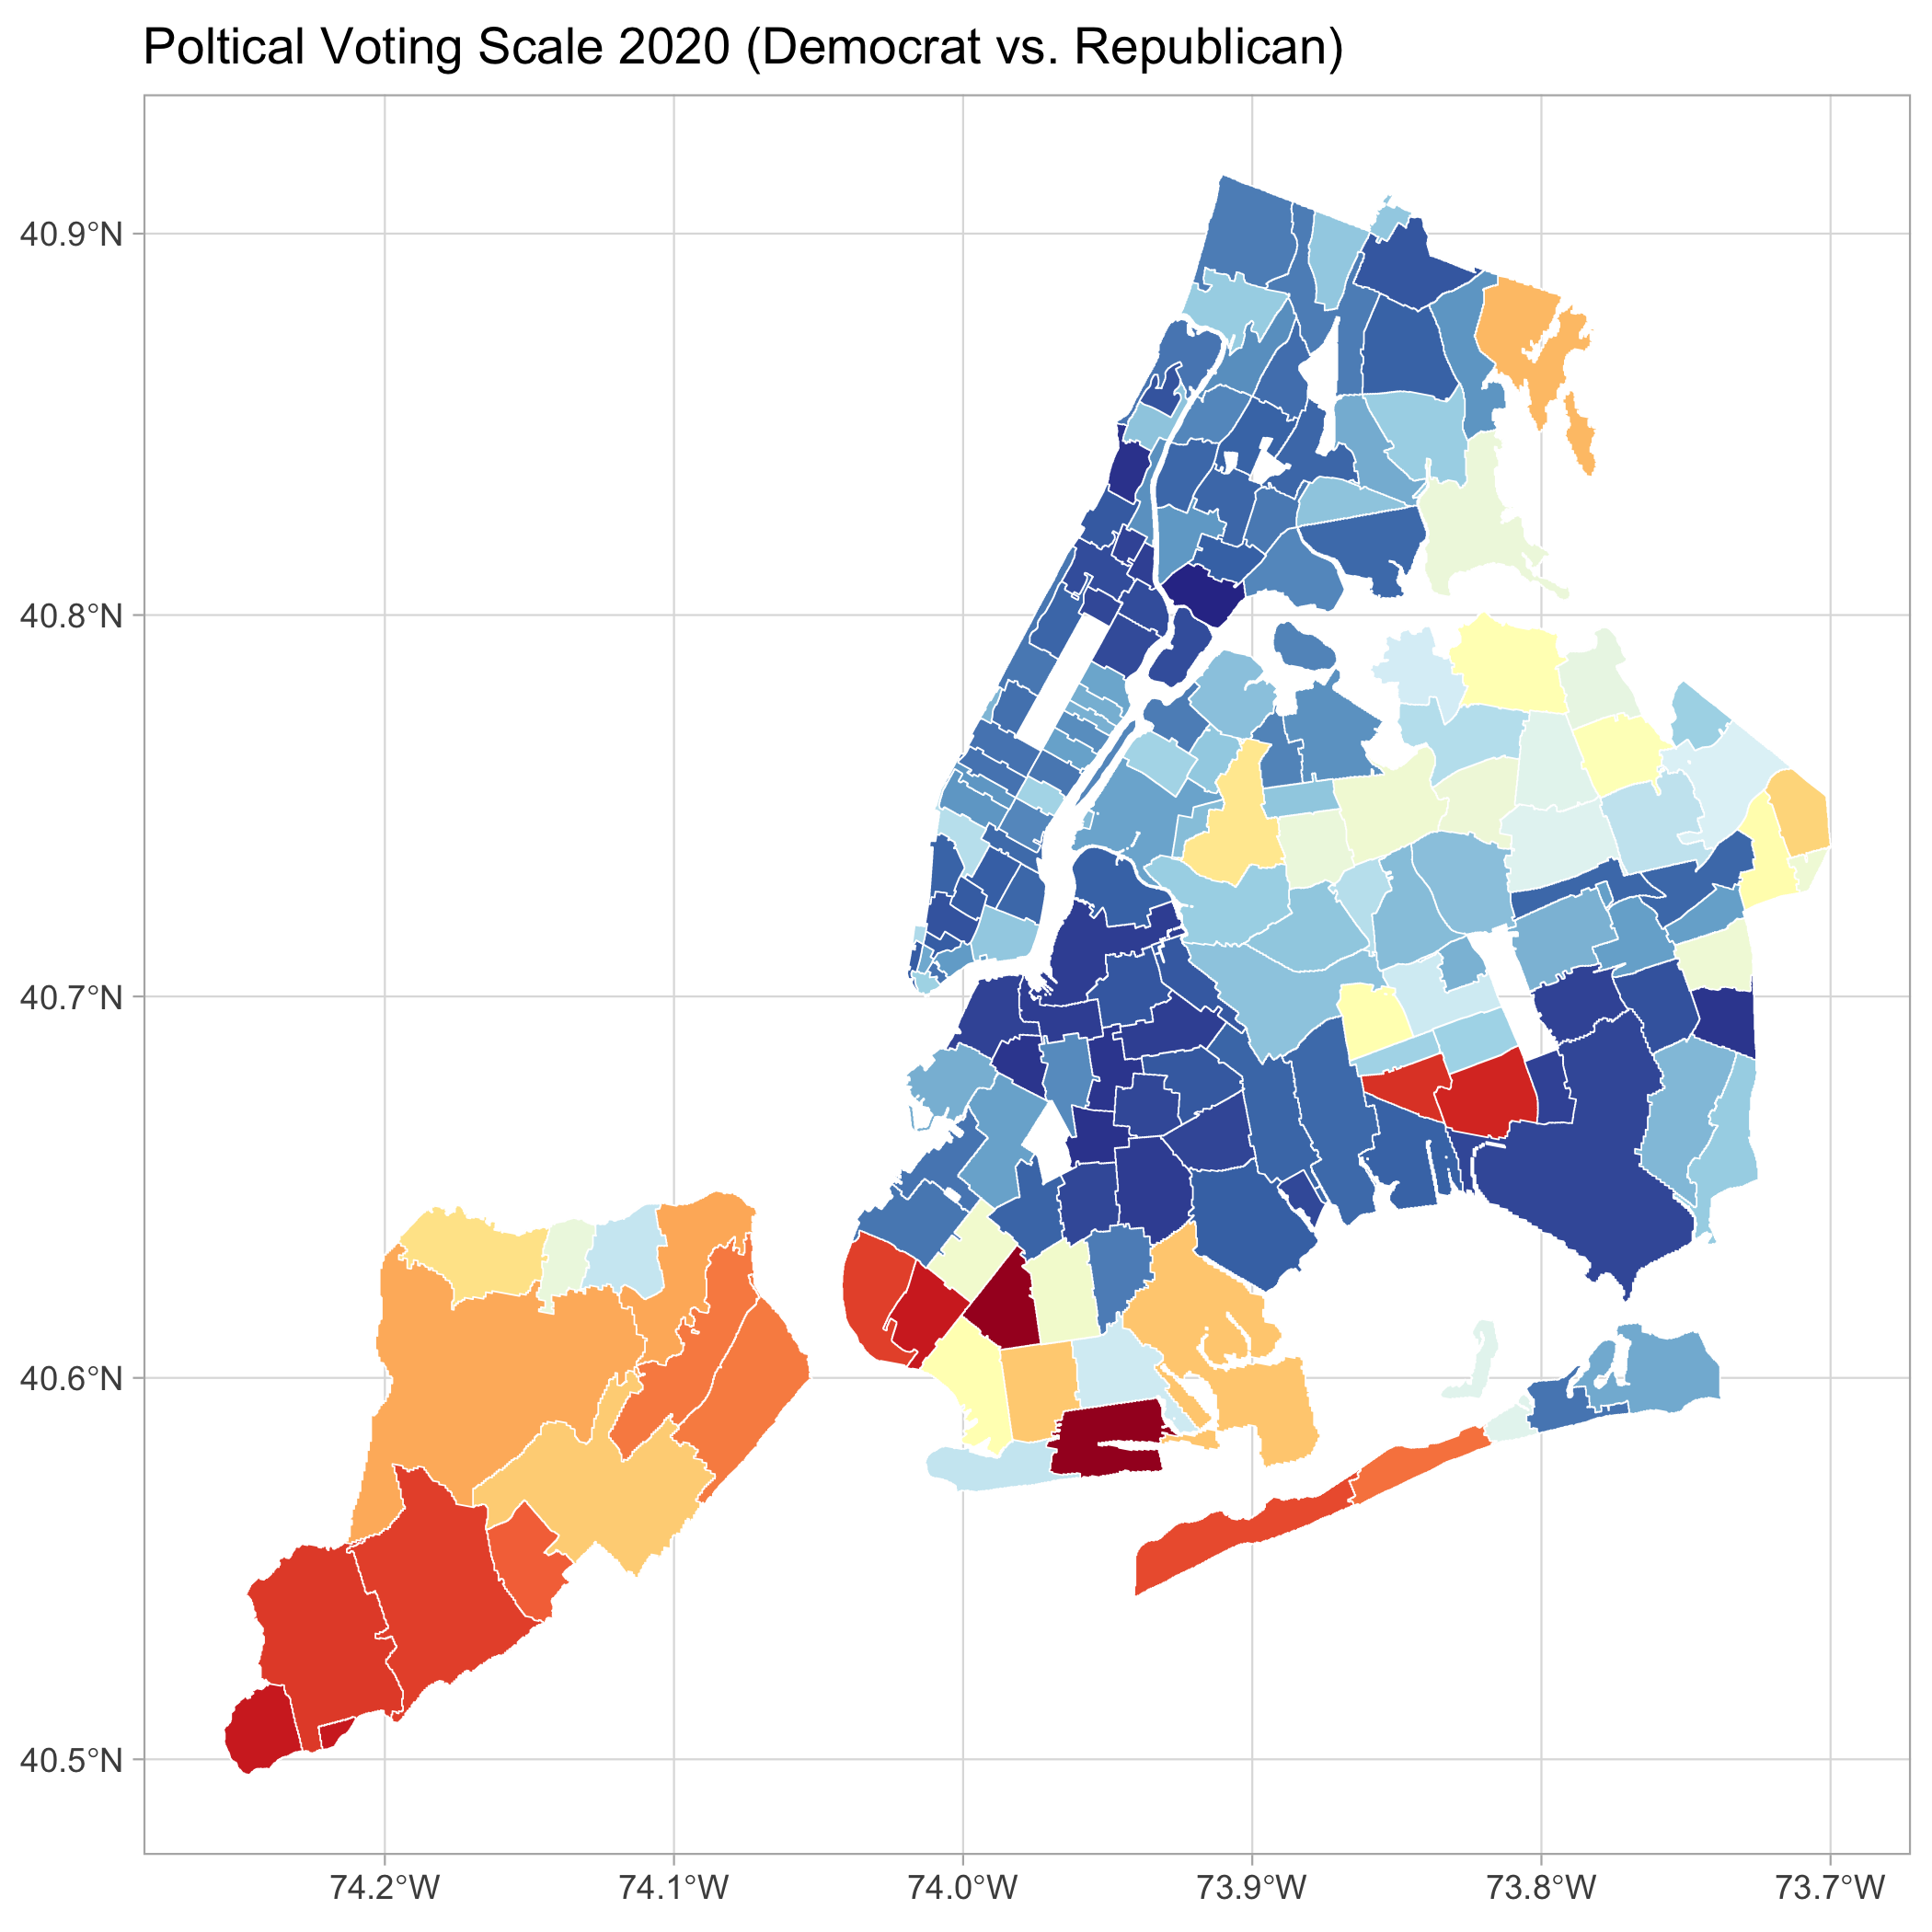
\includegraphics[width=0.45\linewidth]{out/maps/electoral_map_2020_gg.png}\label{ed-2020}}
    \subfloat[2024]{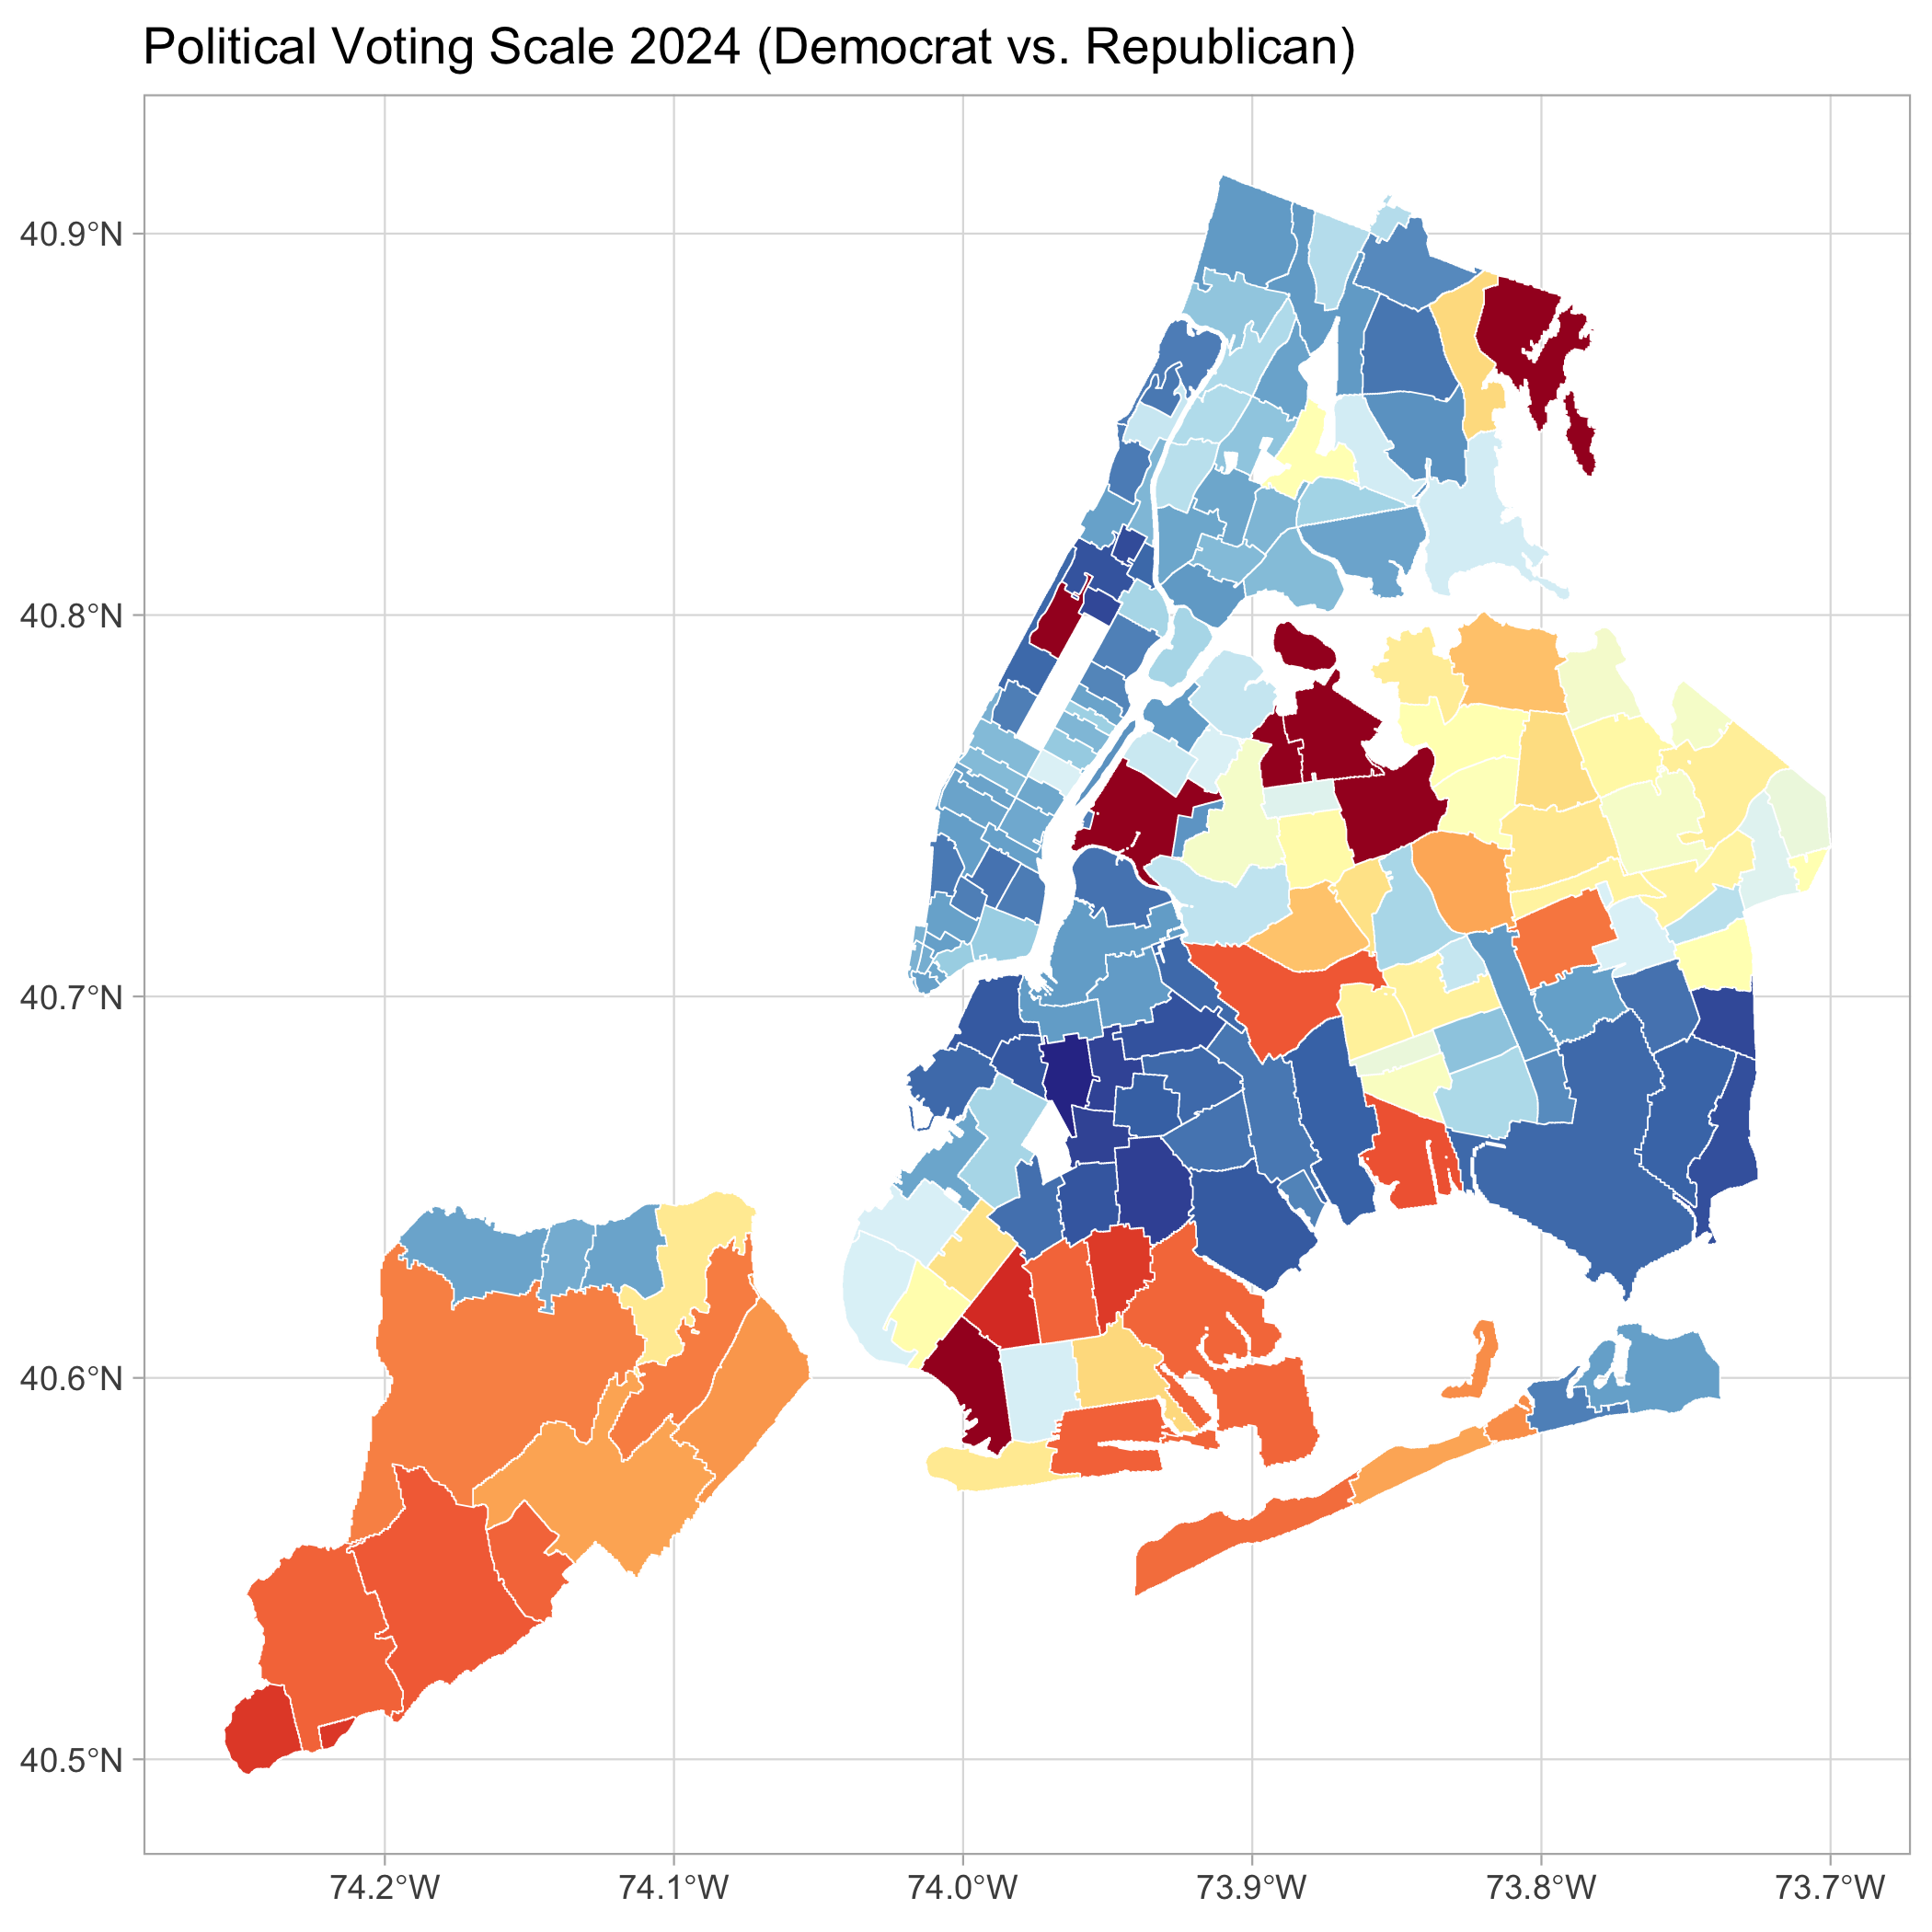
\includegraphics[width=0.45\linewidth]{out/maps/electoral_map_2024_gg.png}\label{ed-2024}}
    \caption{NYC Election Results}
\end{figure*}

\subsection{Correlations}

There were several notable correlations we observed:

\begin{itemize}
    \item \textbf{Political Alignment vs. Case Rate}: In 2020, Democrat voters and case rates were negatively correlated (-0.37, p-value = 1.13E-7), while Republican voters showed a positive correlation. In 2024, the negative correlation for Democrat voters slightly decreased to -0.33 but remained statistically significant.
    \item \textbf{Political Alignment vs. Death Rate}: In 2020, Democrat voting fraction and death rates were negatively correlated (p-value = 0.04). In 2024, the correlation became stronger at -0.2395 (p-value = 1.6E-3).
    \item \textbf{Political Alignment vs. Vaccinations}: There was no significant correlation between vaccination rates and election voting patterns in both 2020 and 2024, indicating equal vaccination behavior across political alignments.
    \item \textbf{Case Rates vs. Fully Vaccinated}: A positive correlation (0.33, p-value = 6.2E-06) was observed, suggesting that higher case rates may lead to increased vaccination rates or that vaccinated individuals might engage in riskier behaviors.
    \item \textbf{Death Rates vs Fully Vaccinated}: There was a negative correlation observed (-0.195, p-value = 0.0093), which is in line with other studies that show that vaccination prevents severe symptoms and provide better outcomes \cite{mohammed-covid-vax-review}.
\end{itemize}

Correlations are summarized in Table \ref{tab:correlations} and visualized in Fig. \ref{fig:corr}.

\begin{table*}[h]
    \centering
    \begin{tabular}{|l|l|r|r|}
        \hline
        \textbf{X} & \textbf{Y} & $R^2$ & \textbf{p-value} \\
        \hline
        Democrat Fraction 2020 & Case Rate & -0.3869 & 1.1336e-07 \\
        Democrat Fraction 2024 & Case Rate & -0.3304 & 9.5669e-06 \\
        Democrat Fraction 2020 & Death Rate & -0.1545 & 0.0406 \\
        Democrat Fraction 2024 & Death Rate & -0.2395 & 0.0016 \\
        Democrat Fraction 2020 & Percent Fully Vaccinated & -0.0225 & 0.7665 \\
        Democrat Fraction 2024 & Percent Fully Vaccinated & 0.0177 & 0.8180 \\
        Percent Fully Vaccinated & Case Rate & 0.3324 & 6.1842e-06 \\
        Percent Fully Vaccinated & Death Rate & -0.195 & 0.0093 \\
        \hline
    \end{tabular}
    \caption{Correlation between Political Alignment and COVID-19 Metrics}
    \label{tab:correlations}
\end{table*}

\begin{figure*}[t]
    \centering
    \subfloat[\centering Case Rates vs Dem Fraction 2020]{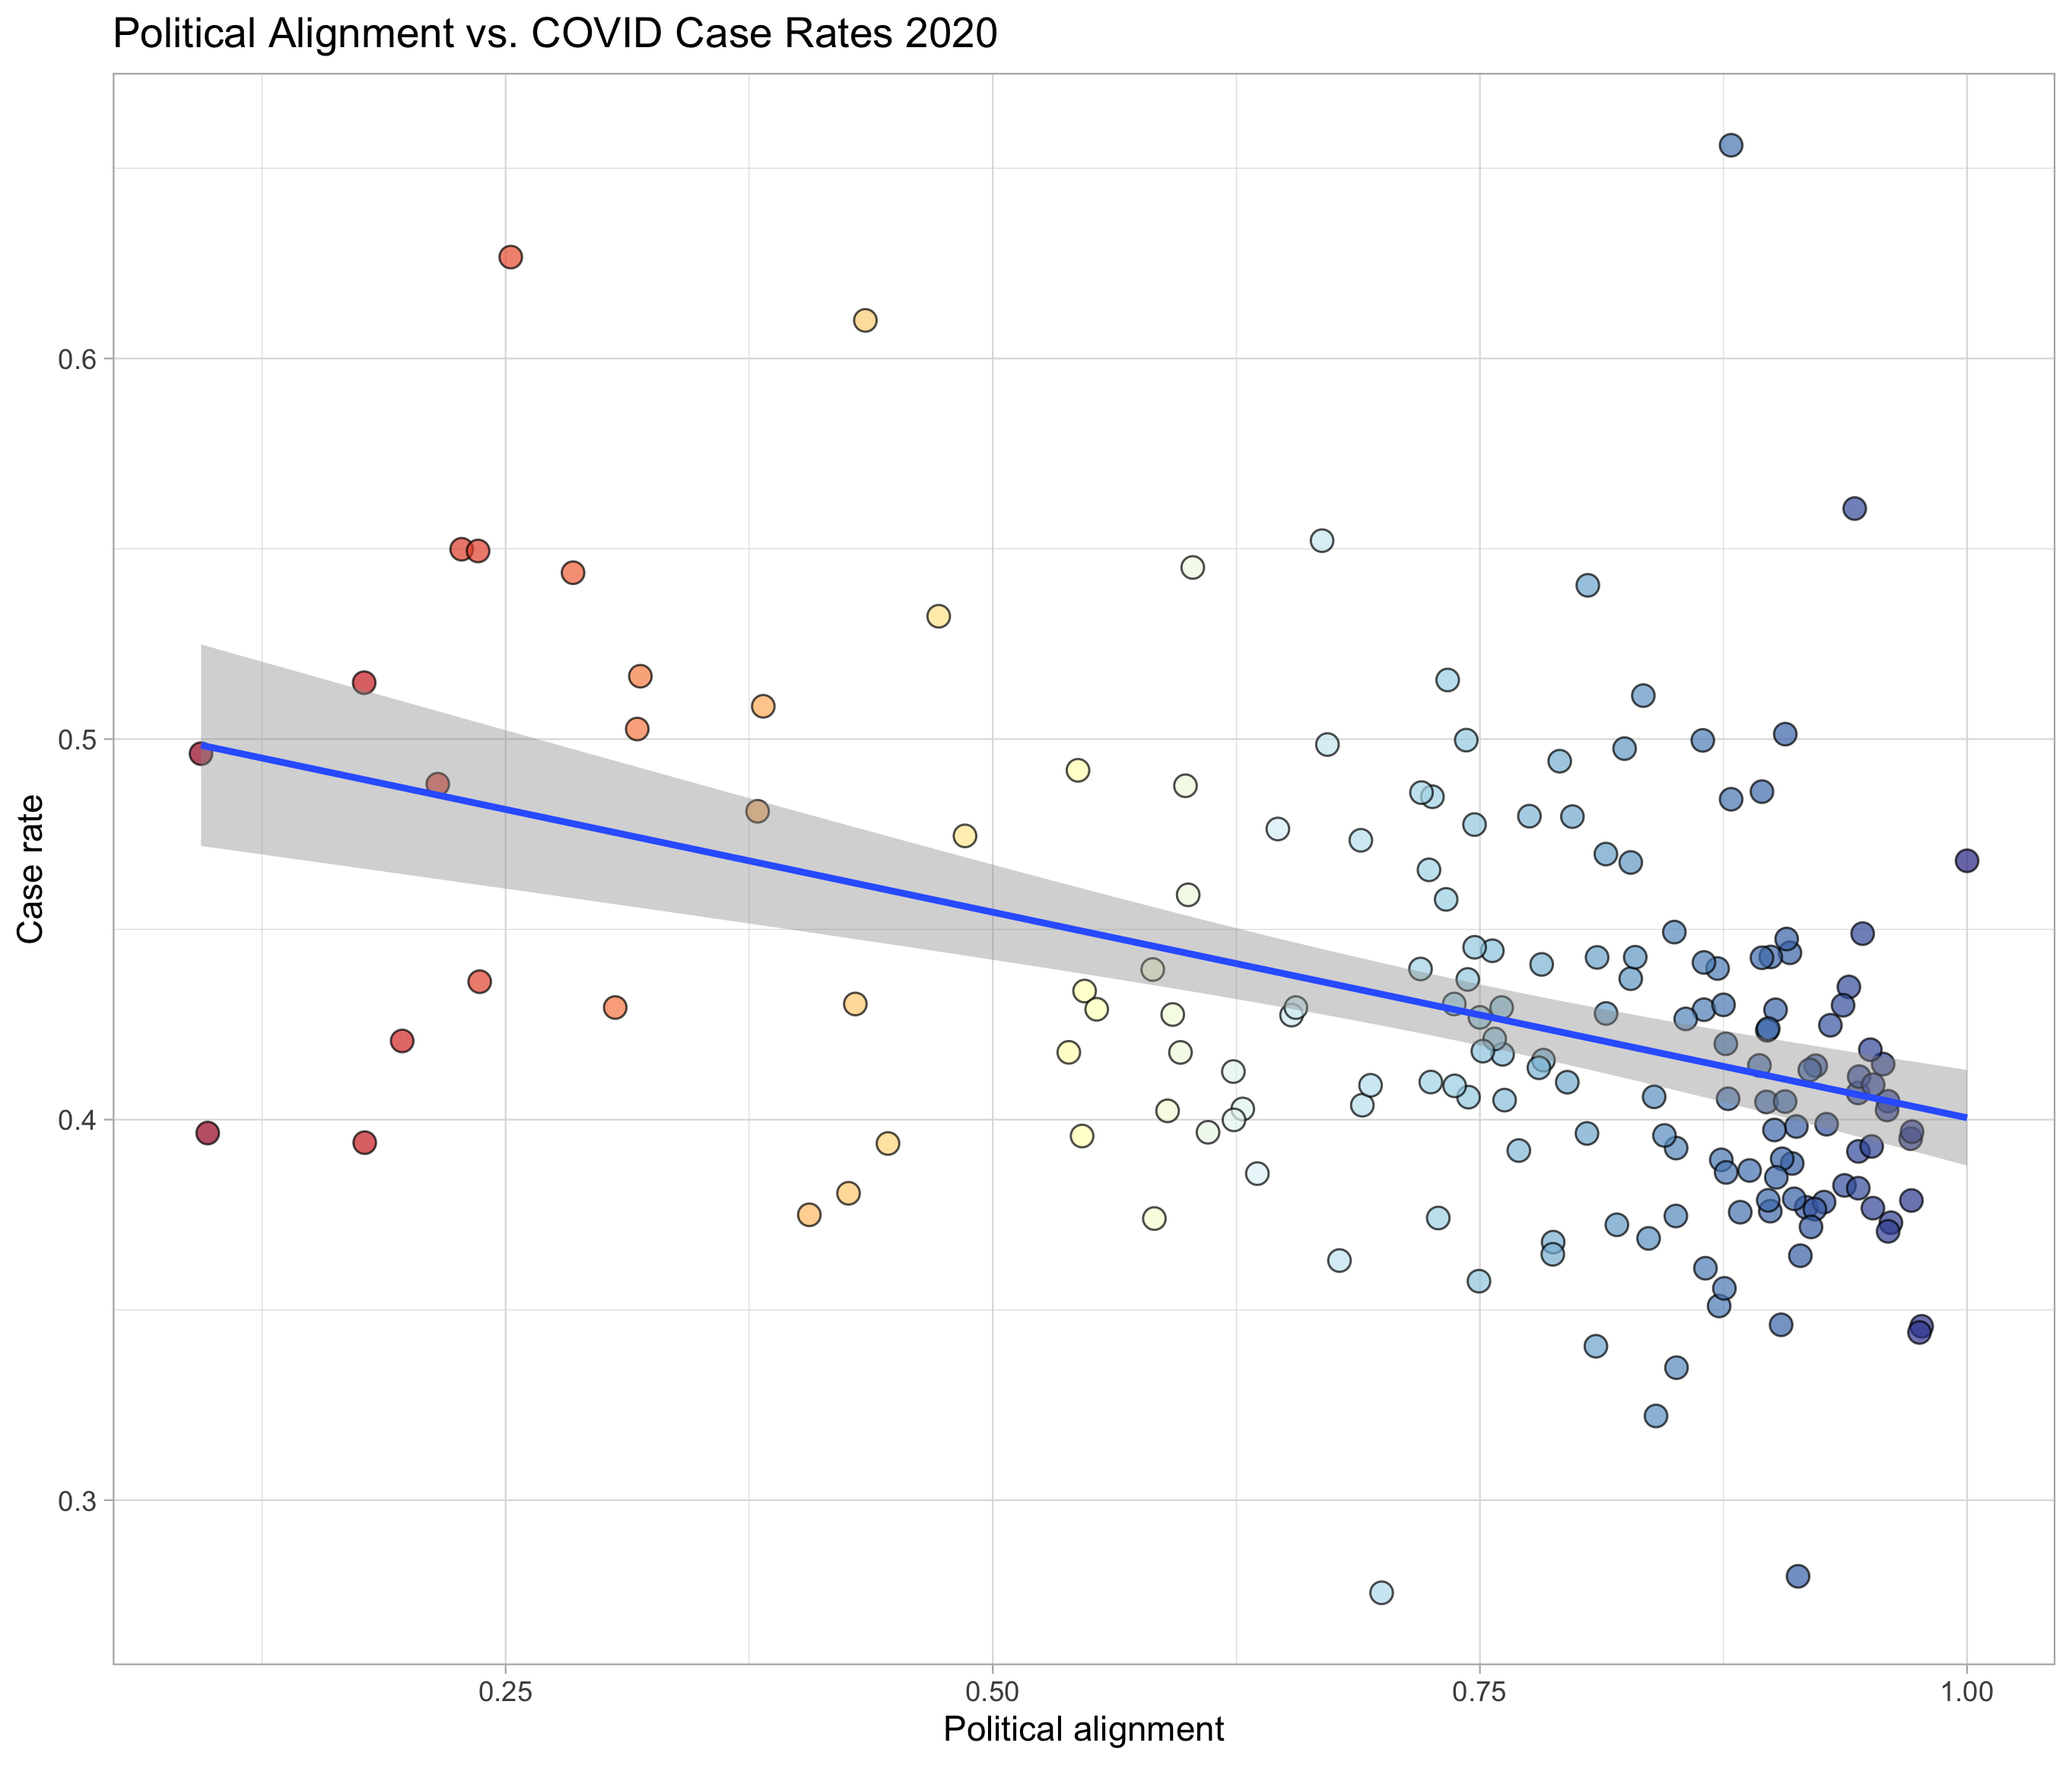
\includegraphics[width=0.25\linewidth]{out/correlations/corr_plot_case_rates_v_pa_2020.png}}
    \subfloat[\centering Case Rates vs. Dem Fraction 2024]{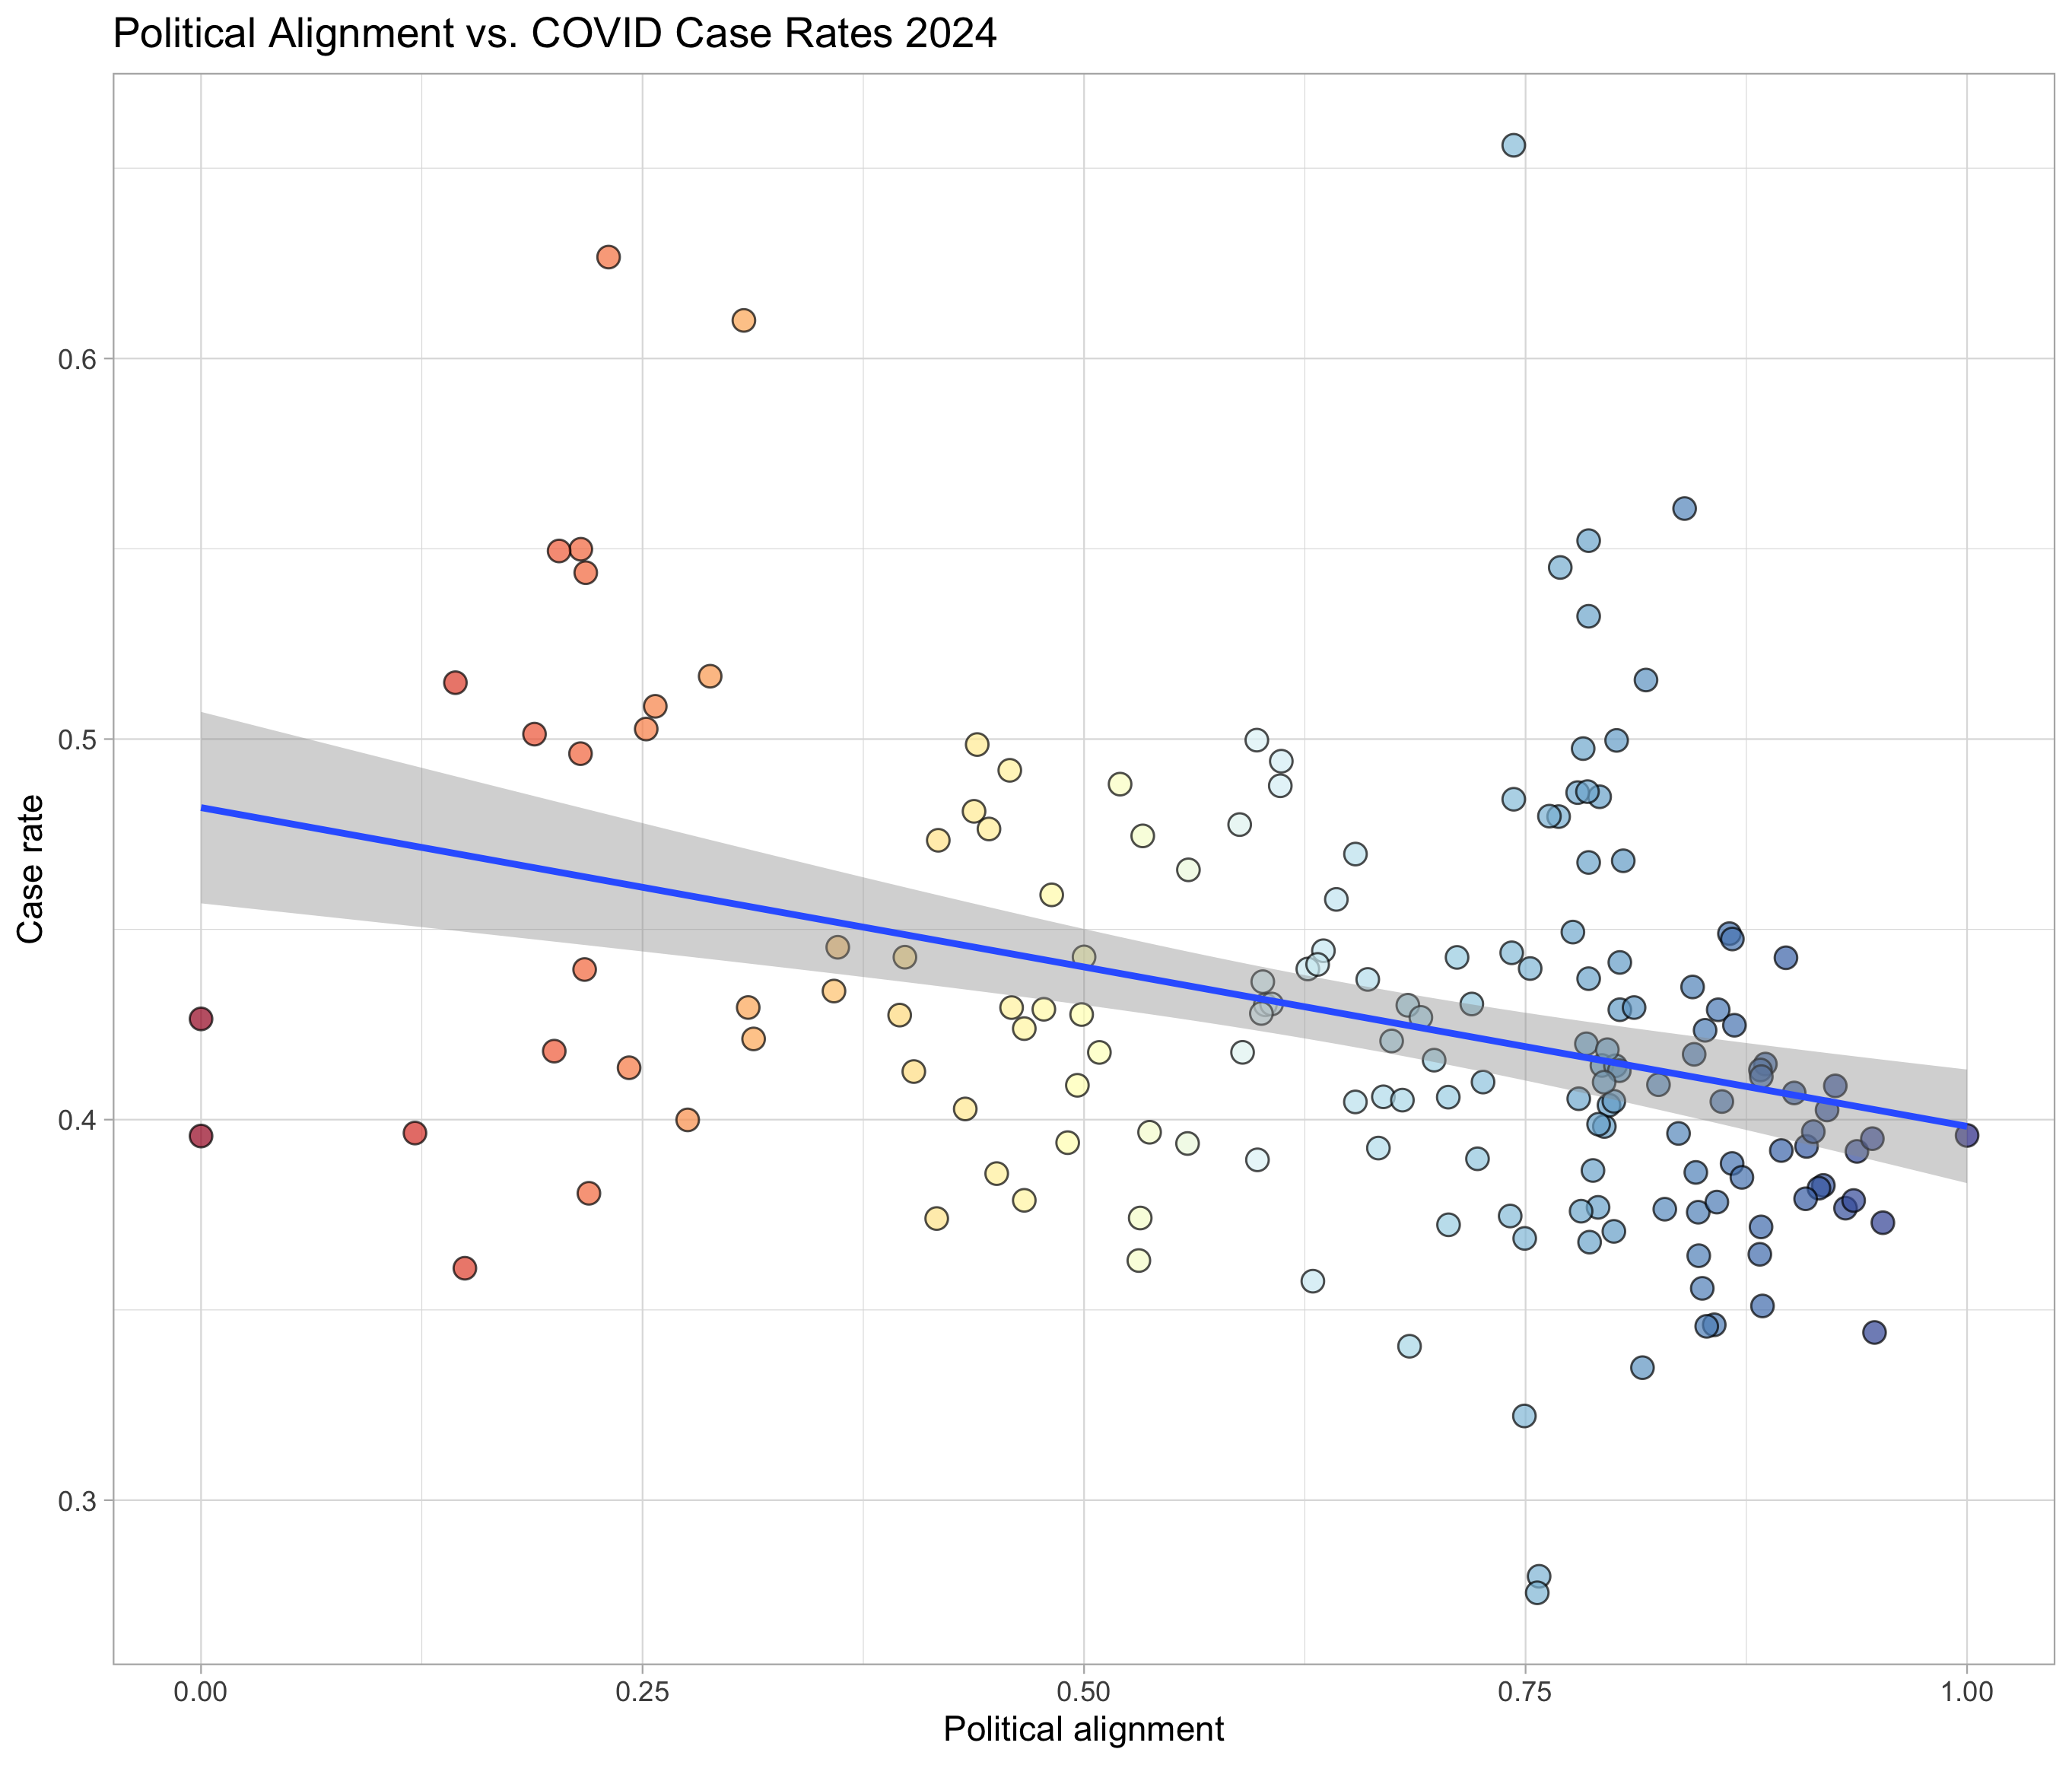
\includegraphics[width=0.25\linewidth]{out/correlations/corr_plot_case_rates_v_pa_2024.png}}
    \subfloat[\centering Death Rates vs. Dem Fraction 2020] {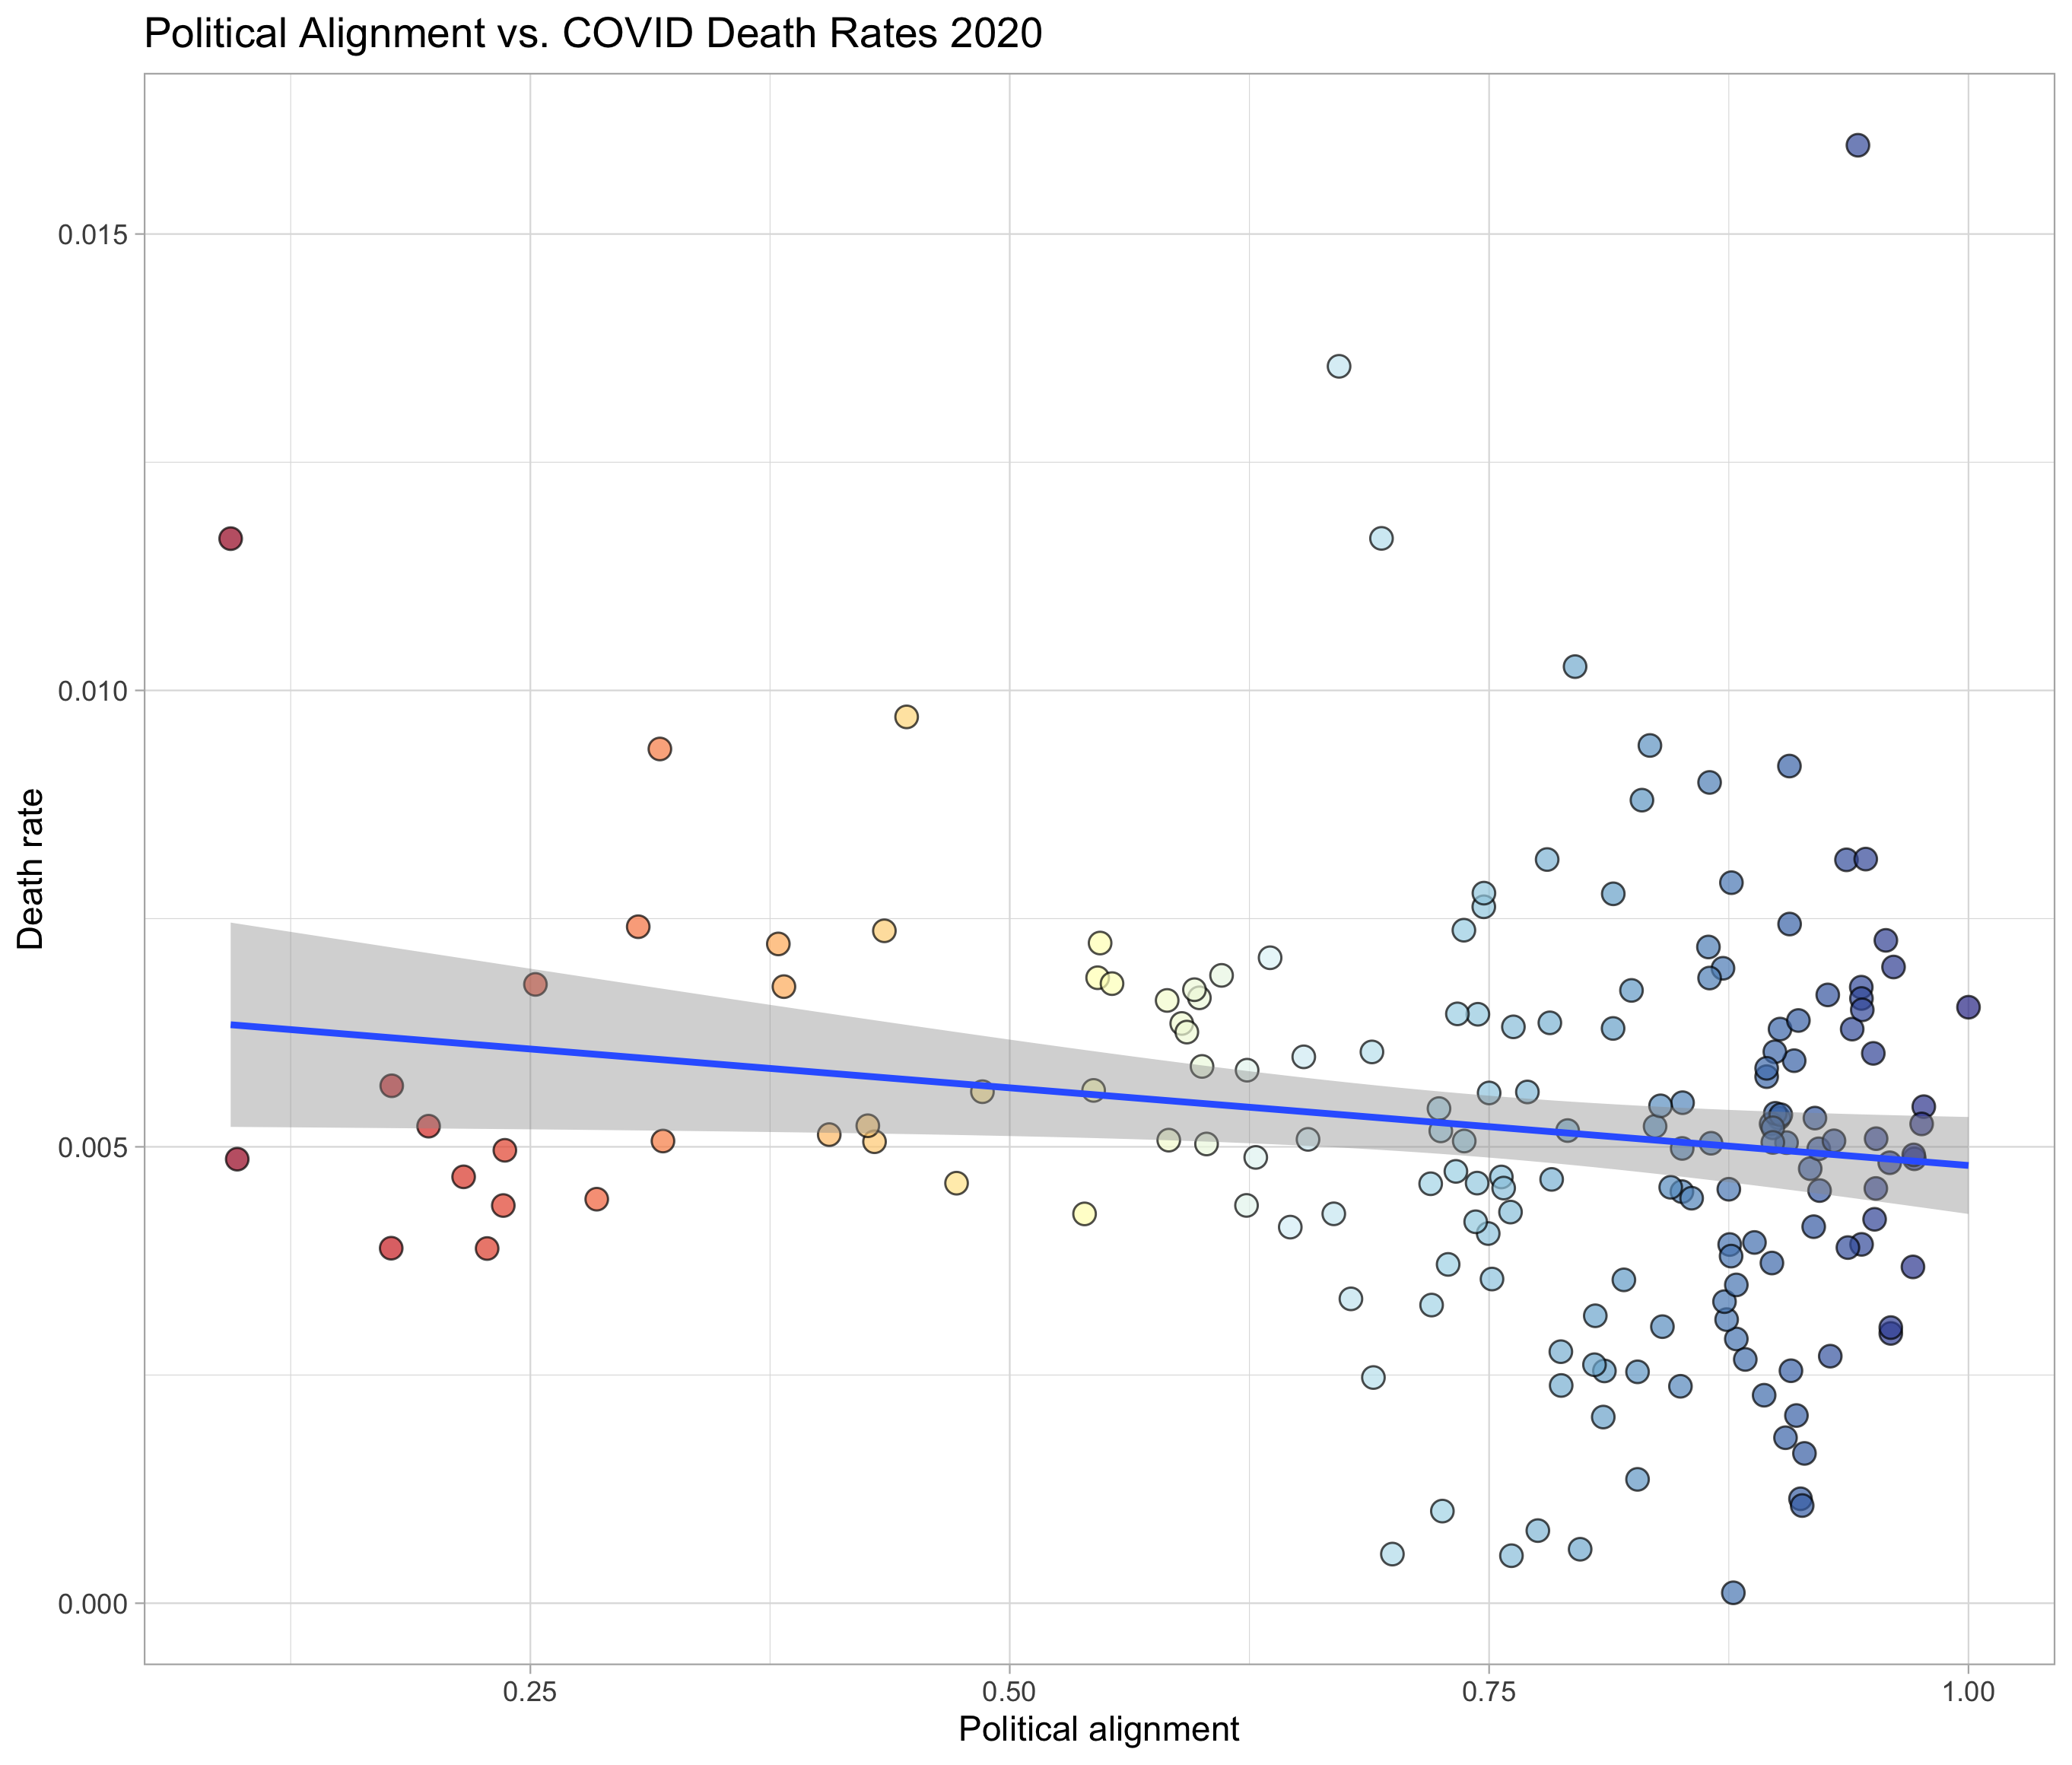
\includegraphics[width=0.25\linewidth]{out/correlations/corr_plot_death_rates_v_pa_2020.png}}
    \subfloat[\centering Death Rates vs. Dem Fraction 2024]{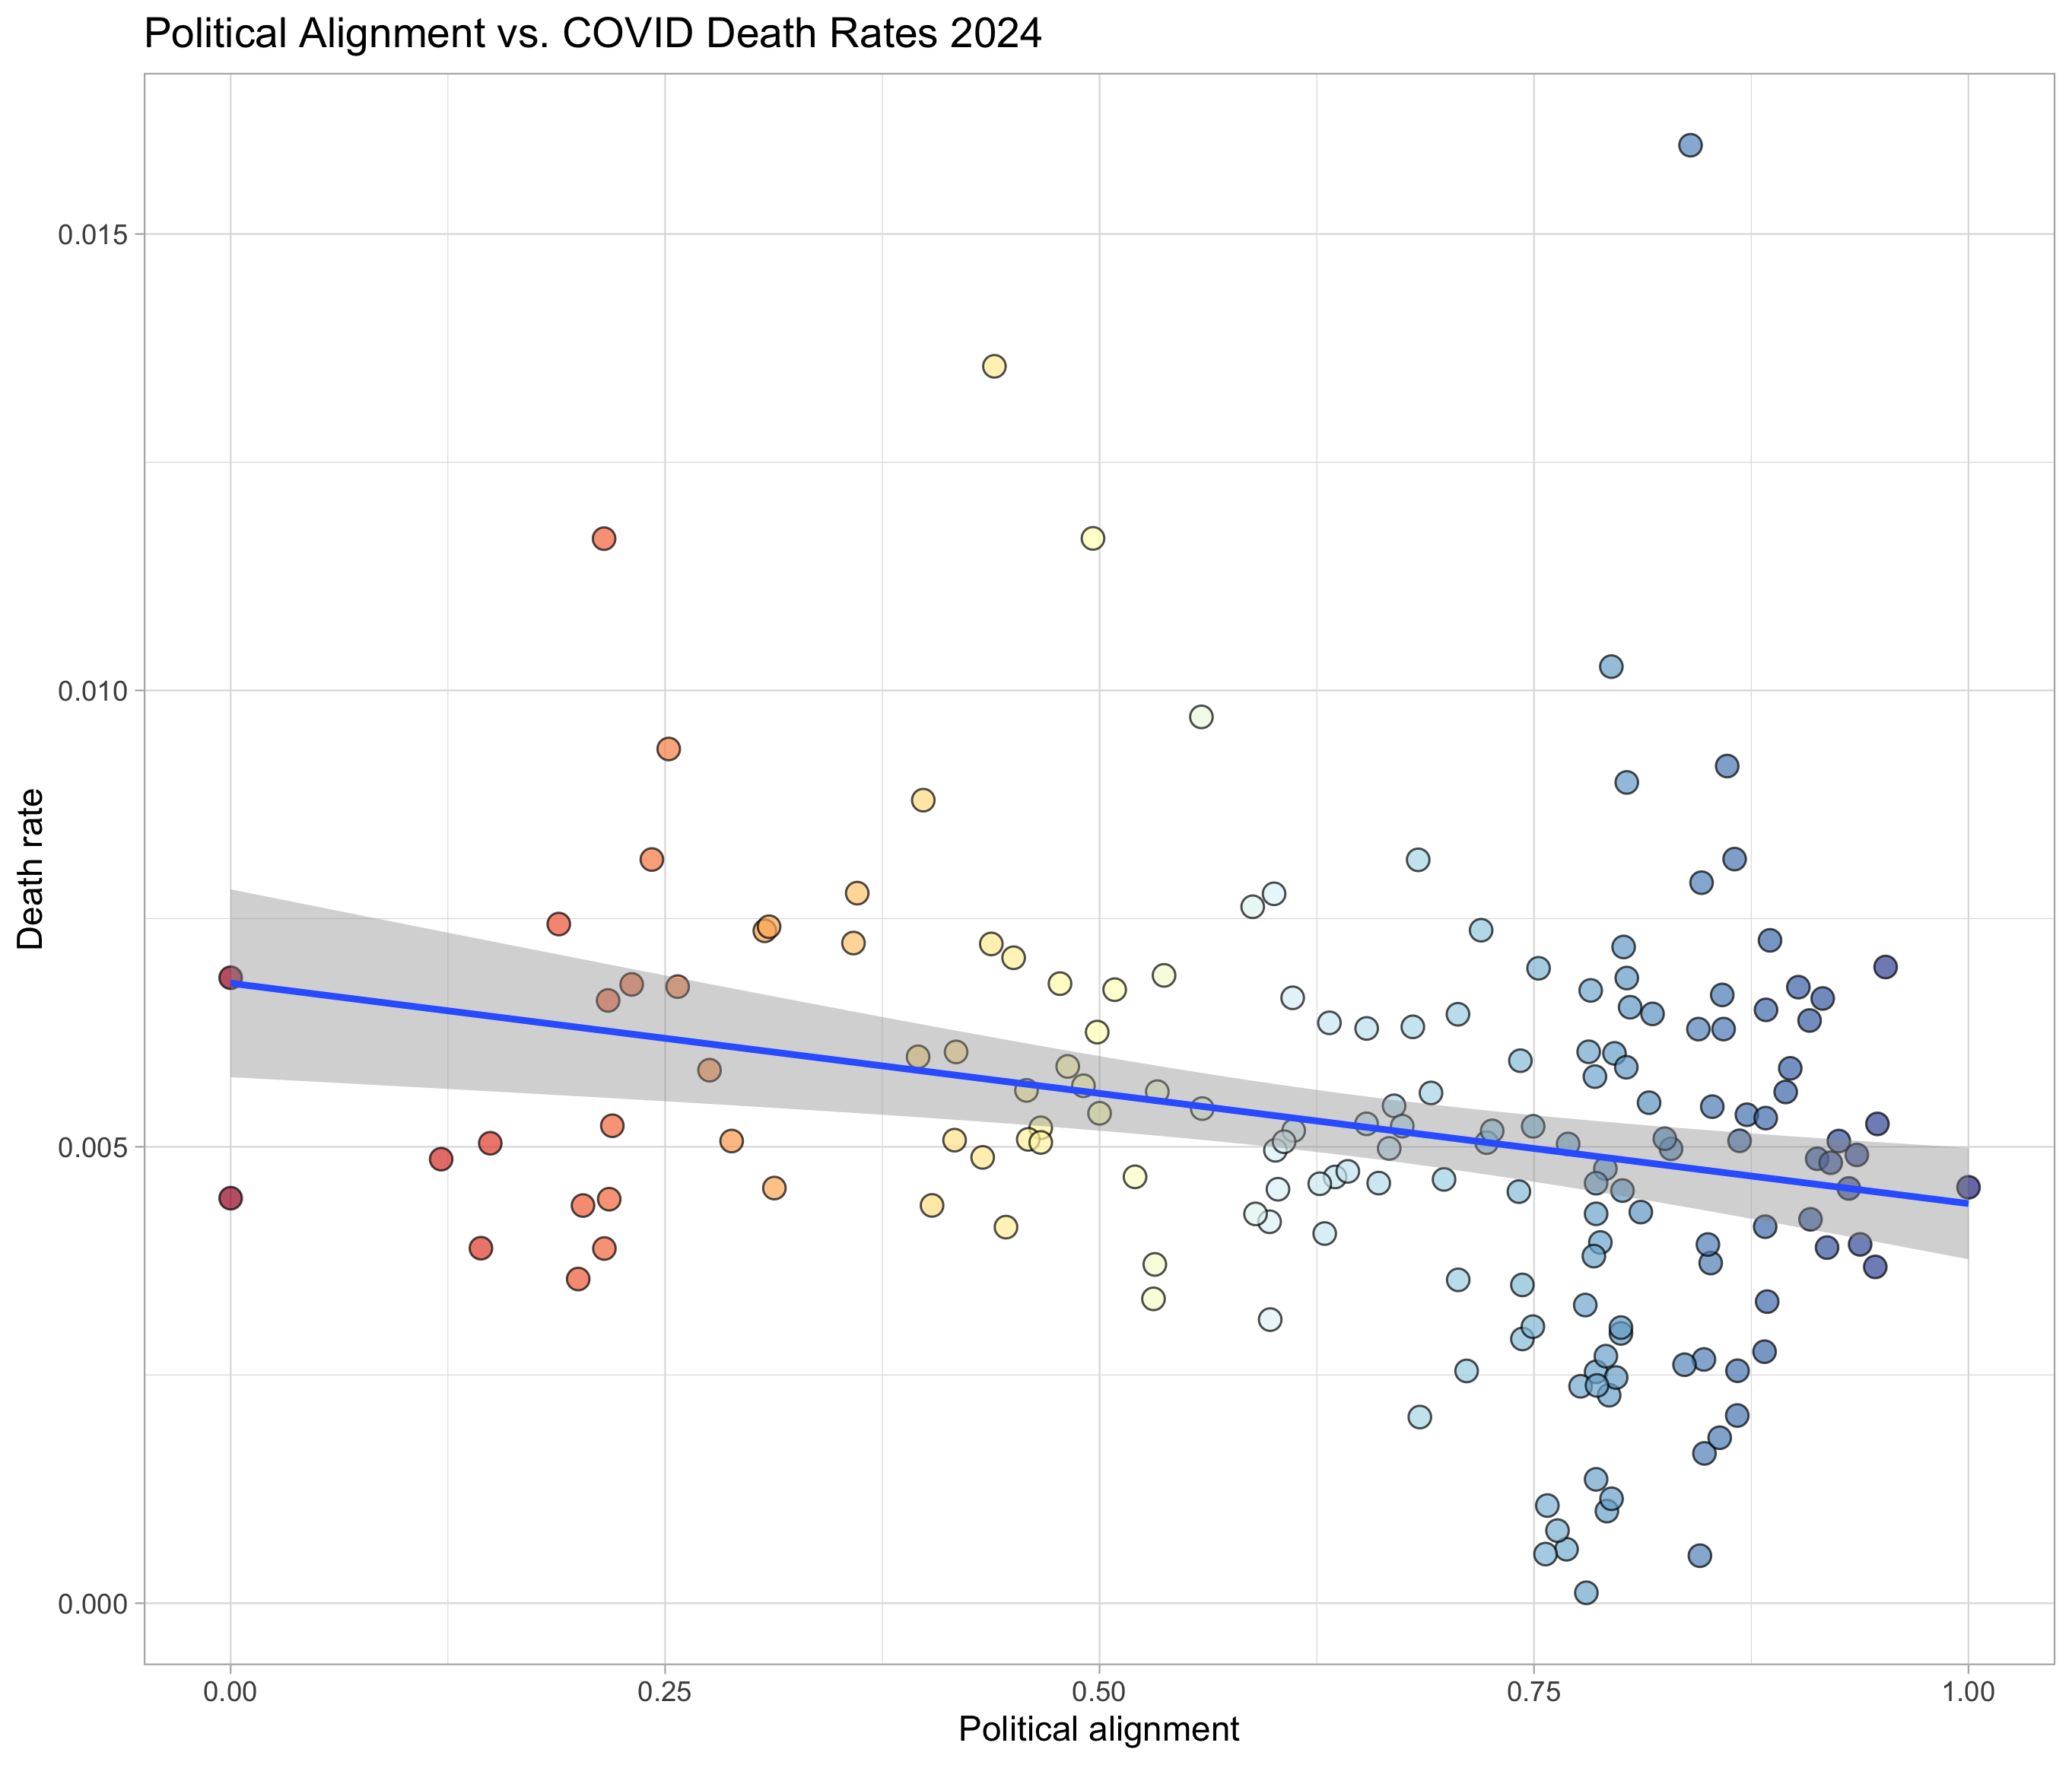
\includegraphics[width=0.25\linewidth]{out/correlations/corr_plot_death_rates_v_pa_2024.png}} \\
    \subfloat[\centering Vaccination Rates vs. Dem Fraction 2020]{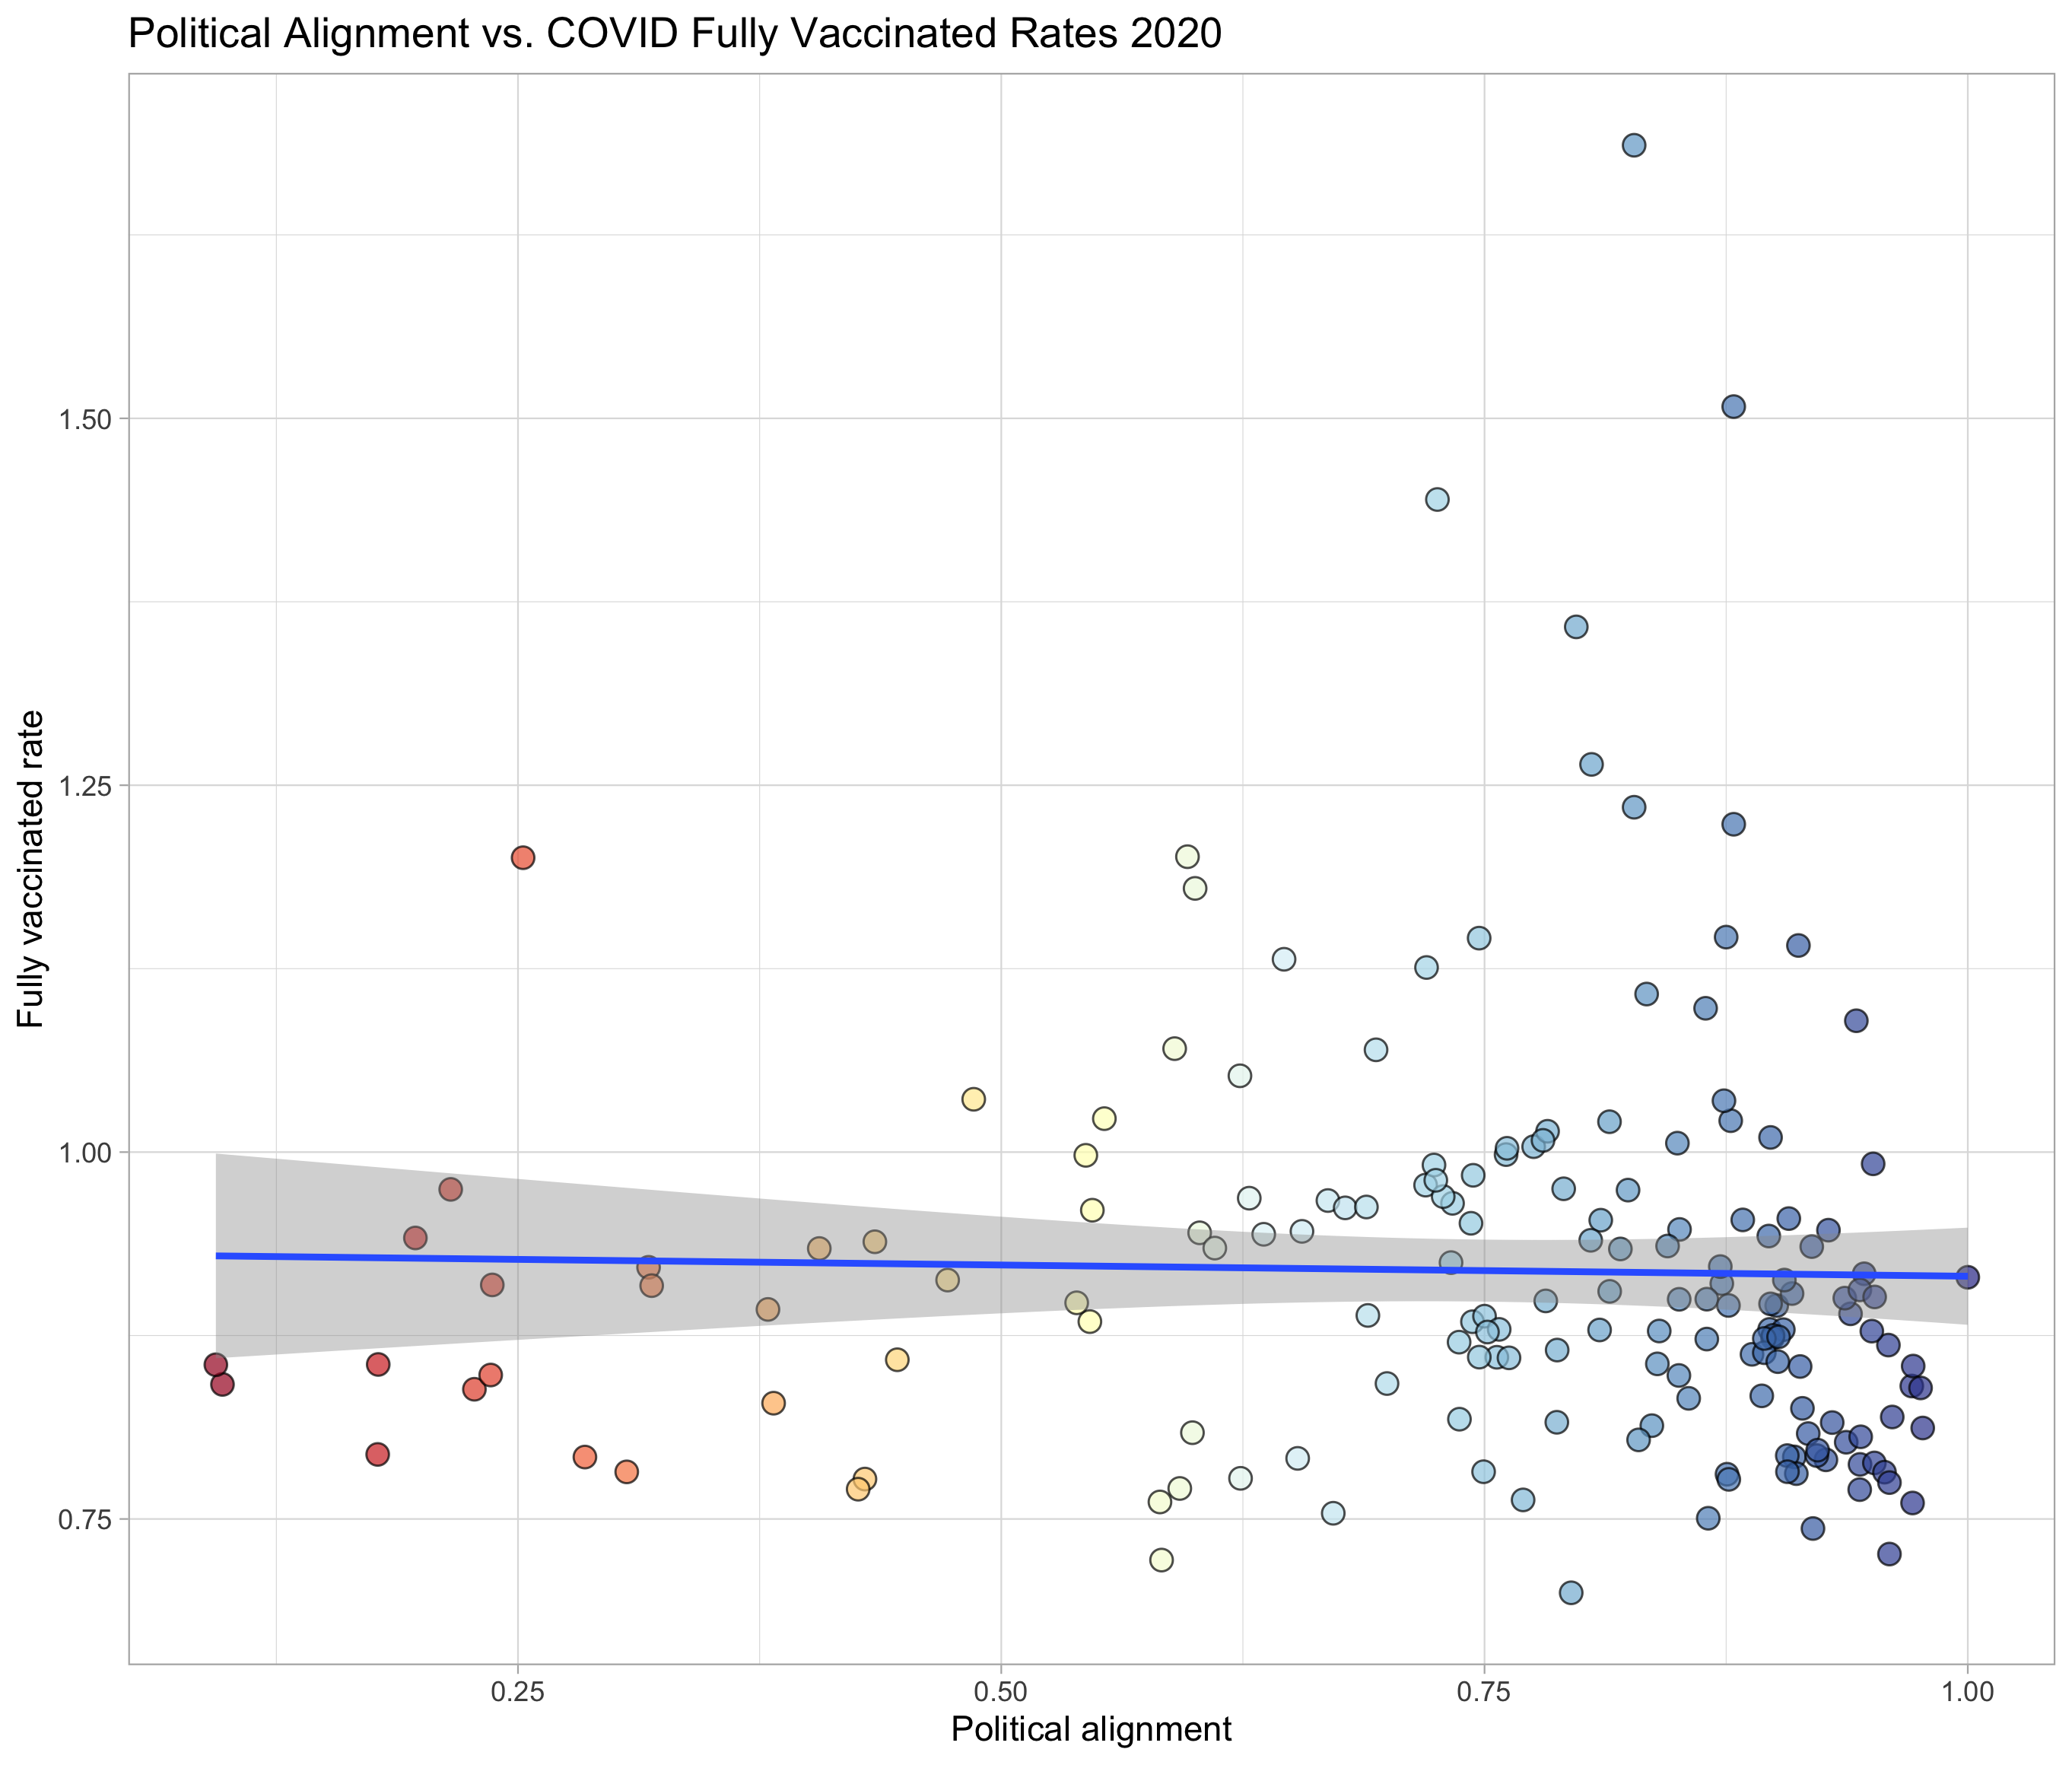
\includegraphics[width=0.25\linewidth]{out/correlations/corr_plot_vax_rates_v_pa_2020.png}}
    \subfloat[\centering Vaccination Rates vs. Dem Fraction 2024]{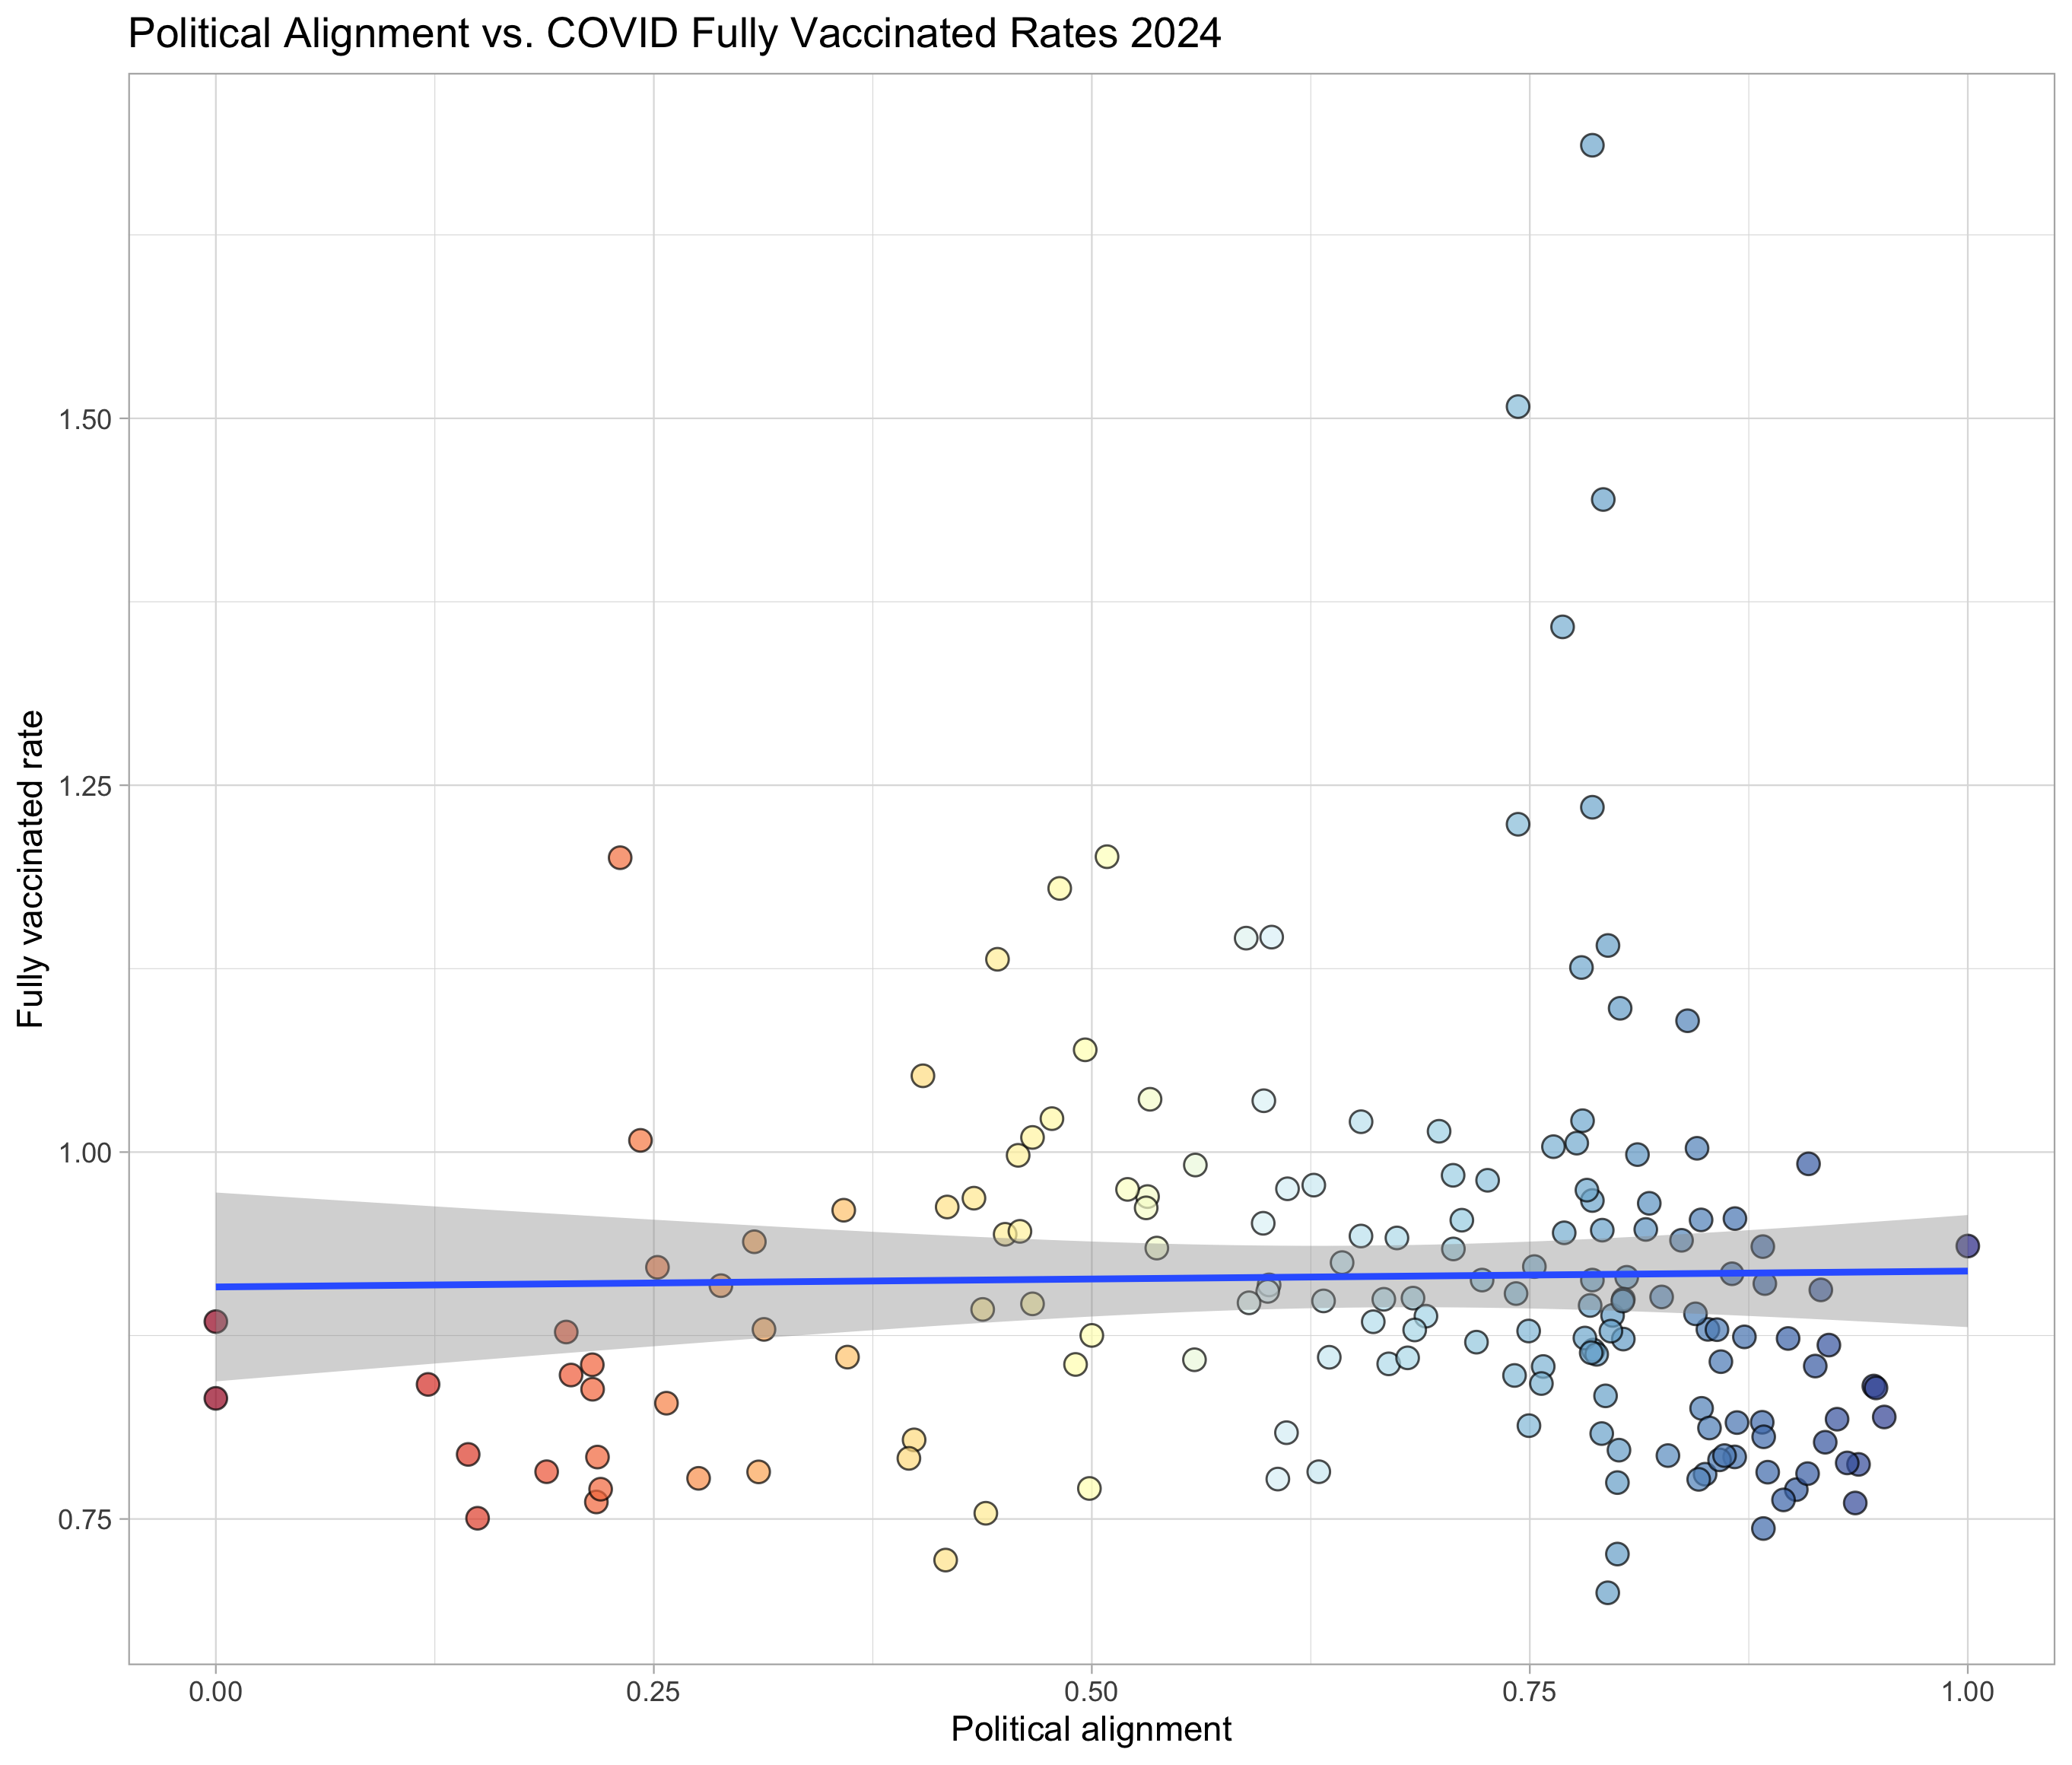
\includegraphics[width=0.25\linewidth]{out/correlations/corr_plot_vax_rates_v_pa_2024.png}} 
    \subfloat[\centering Vaccination Rates vs. Case Rate]{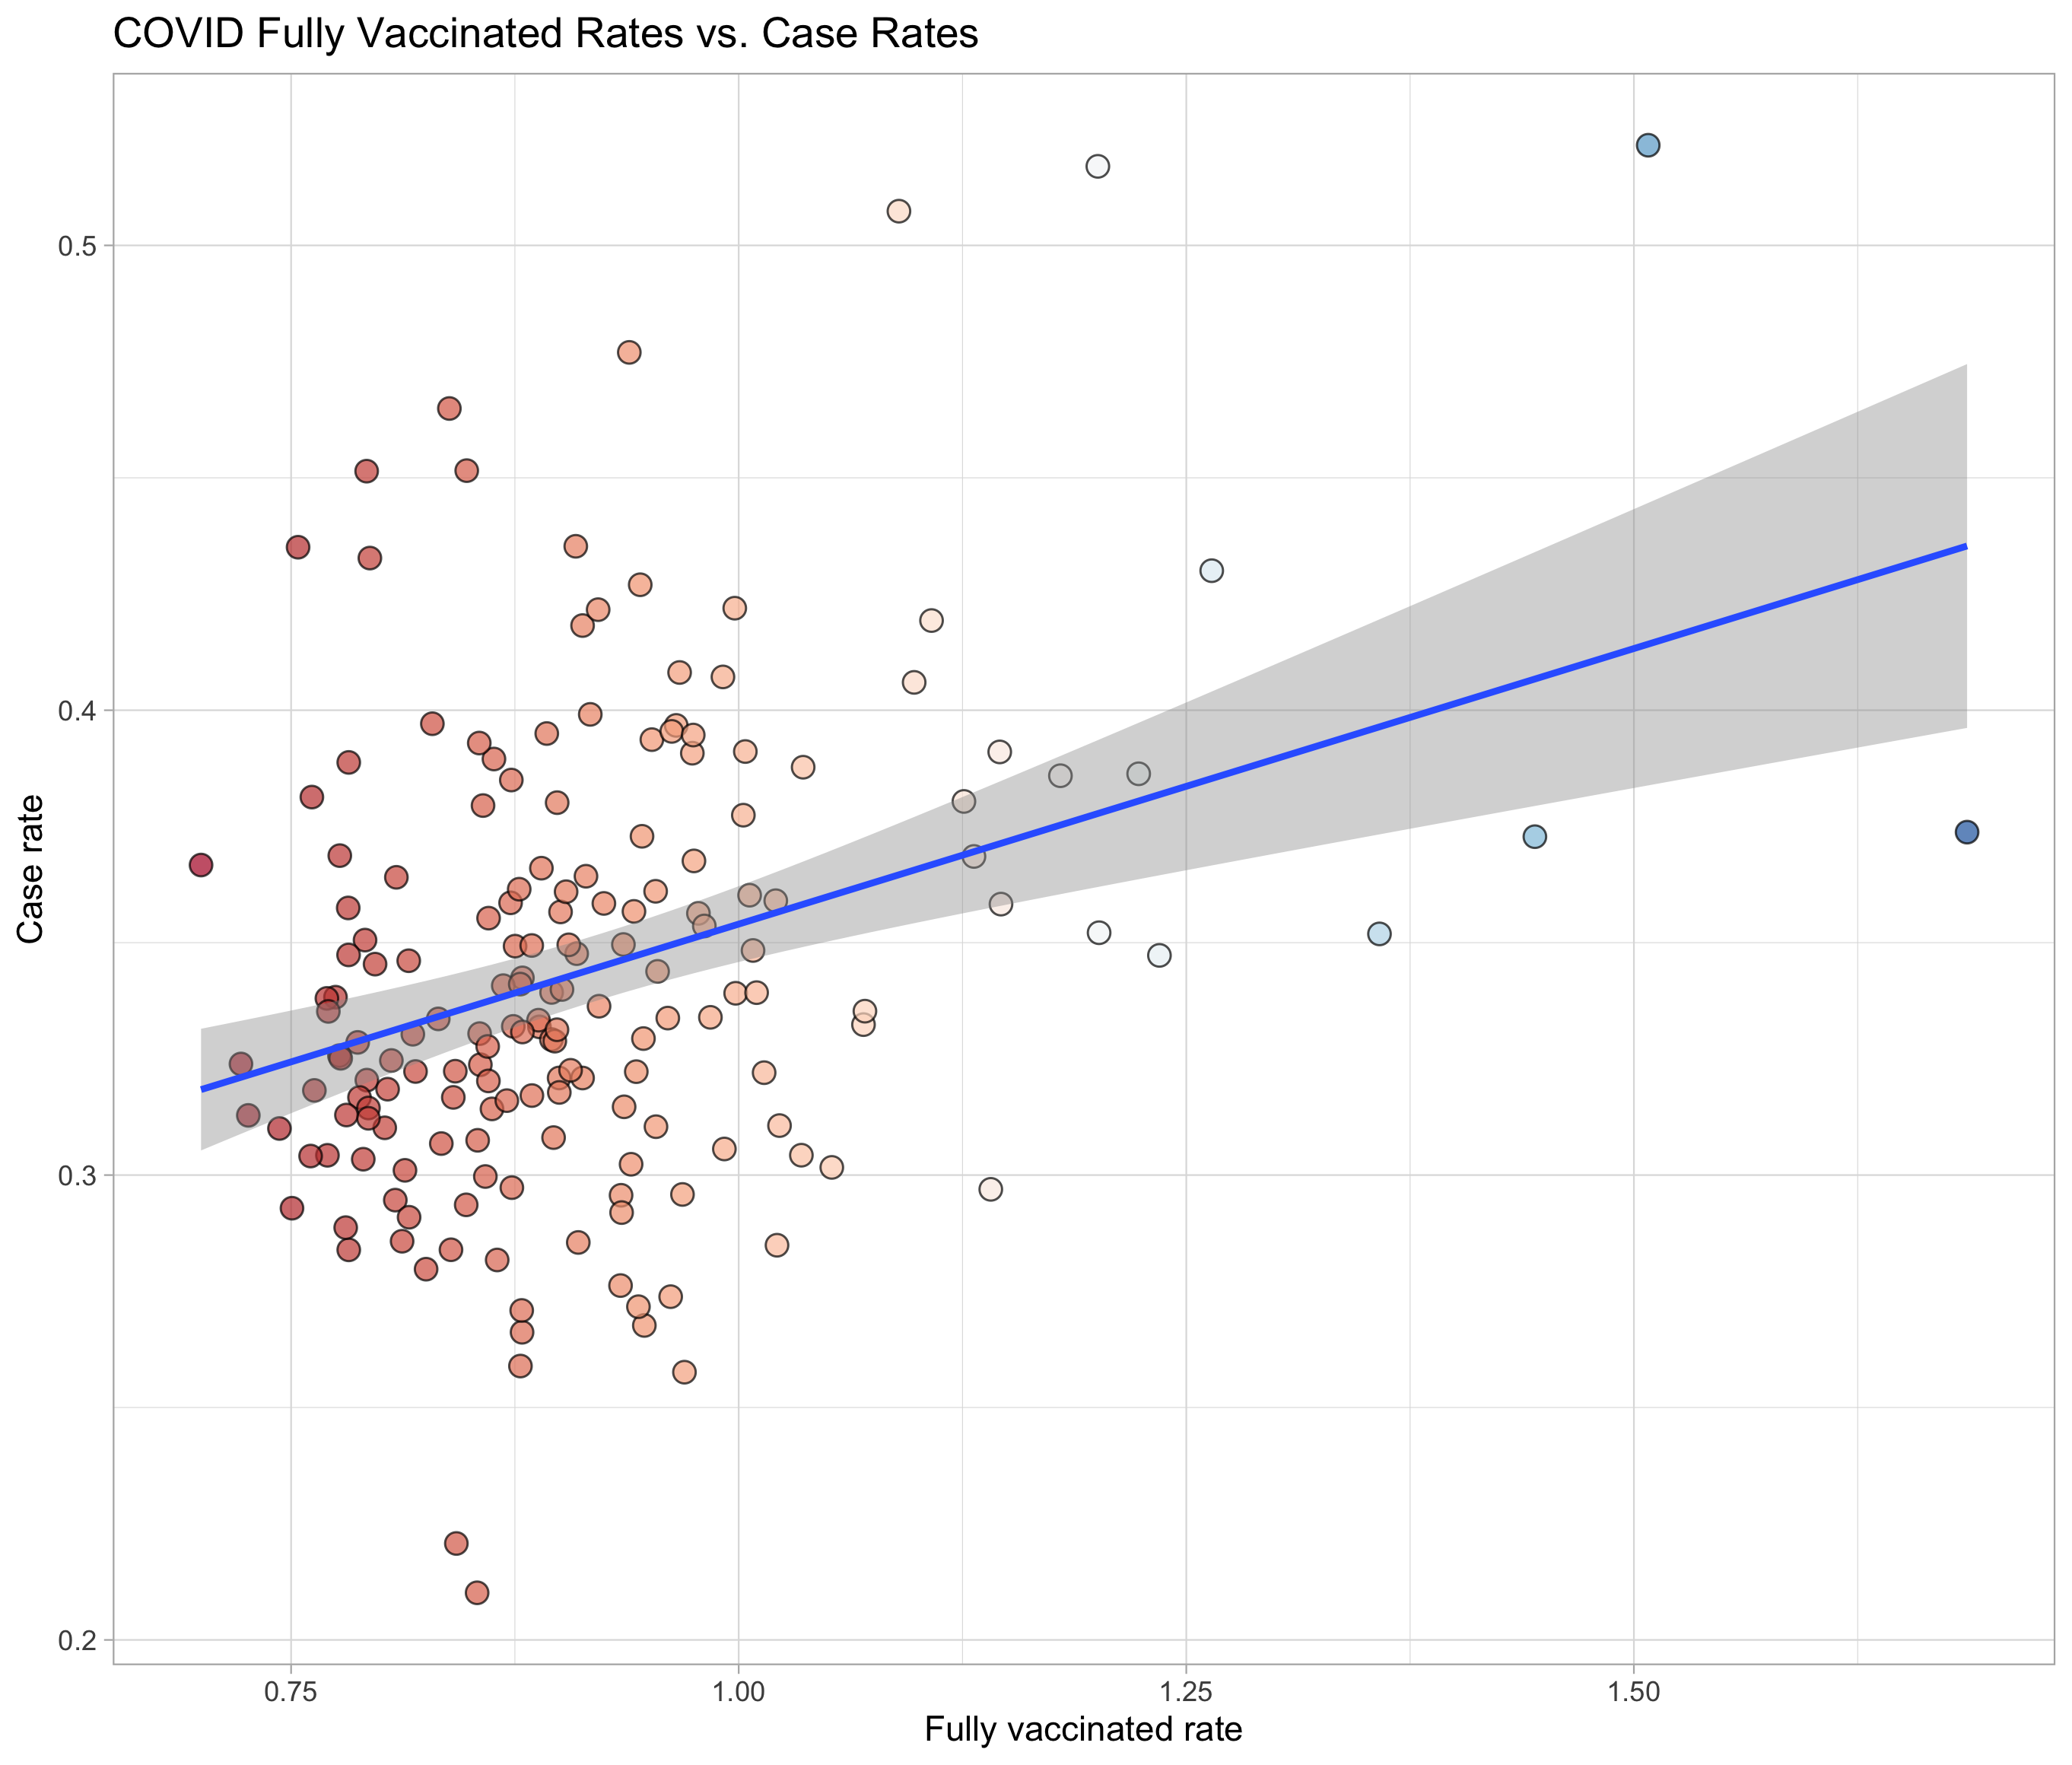
\includegraphics[width=0.25\linewidth]{out/correlations/corr_plot_vax_rates_v_case_rate.png}}
    \subfloat[\centering Vaccination Rates vs. Death Rate]{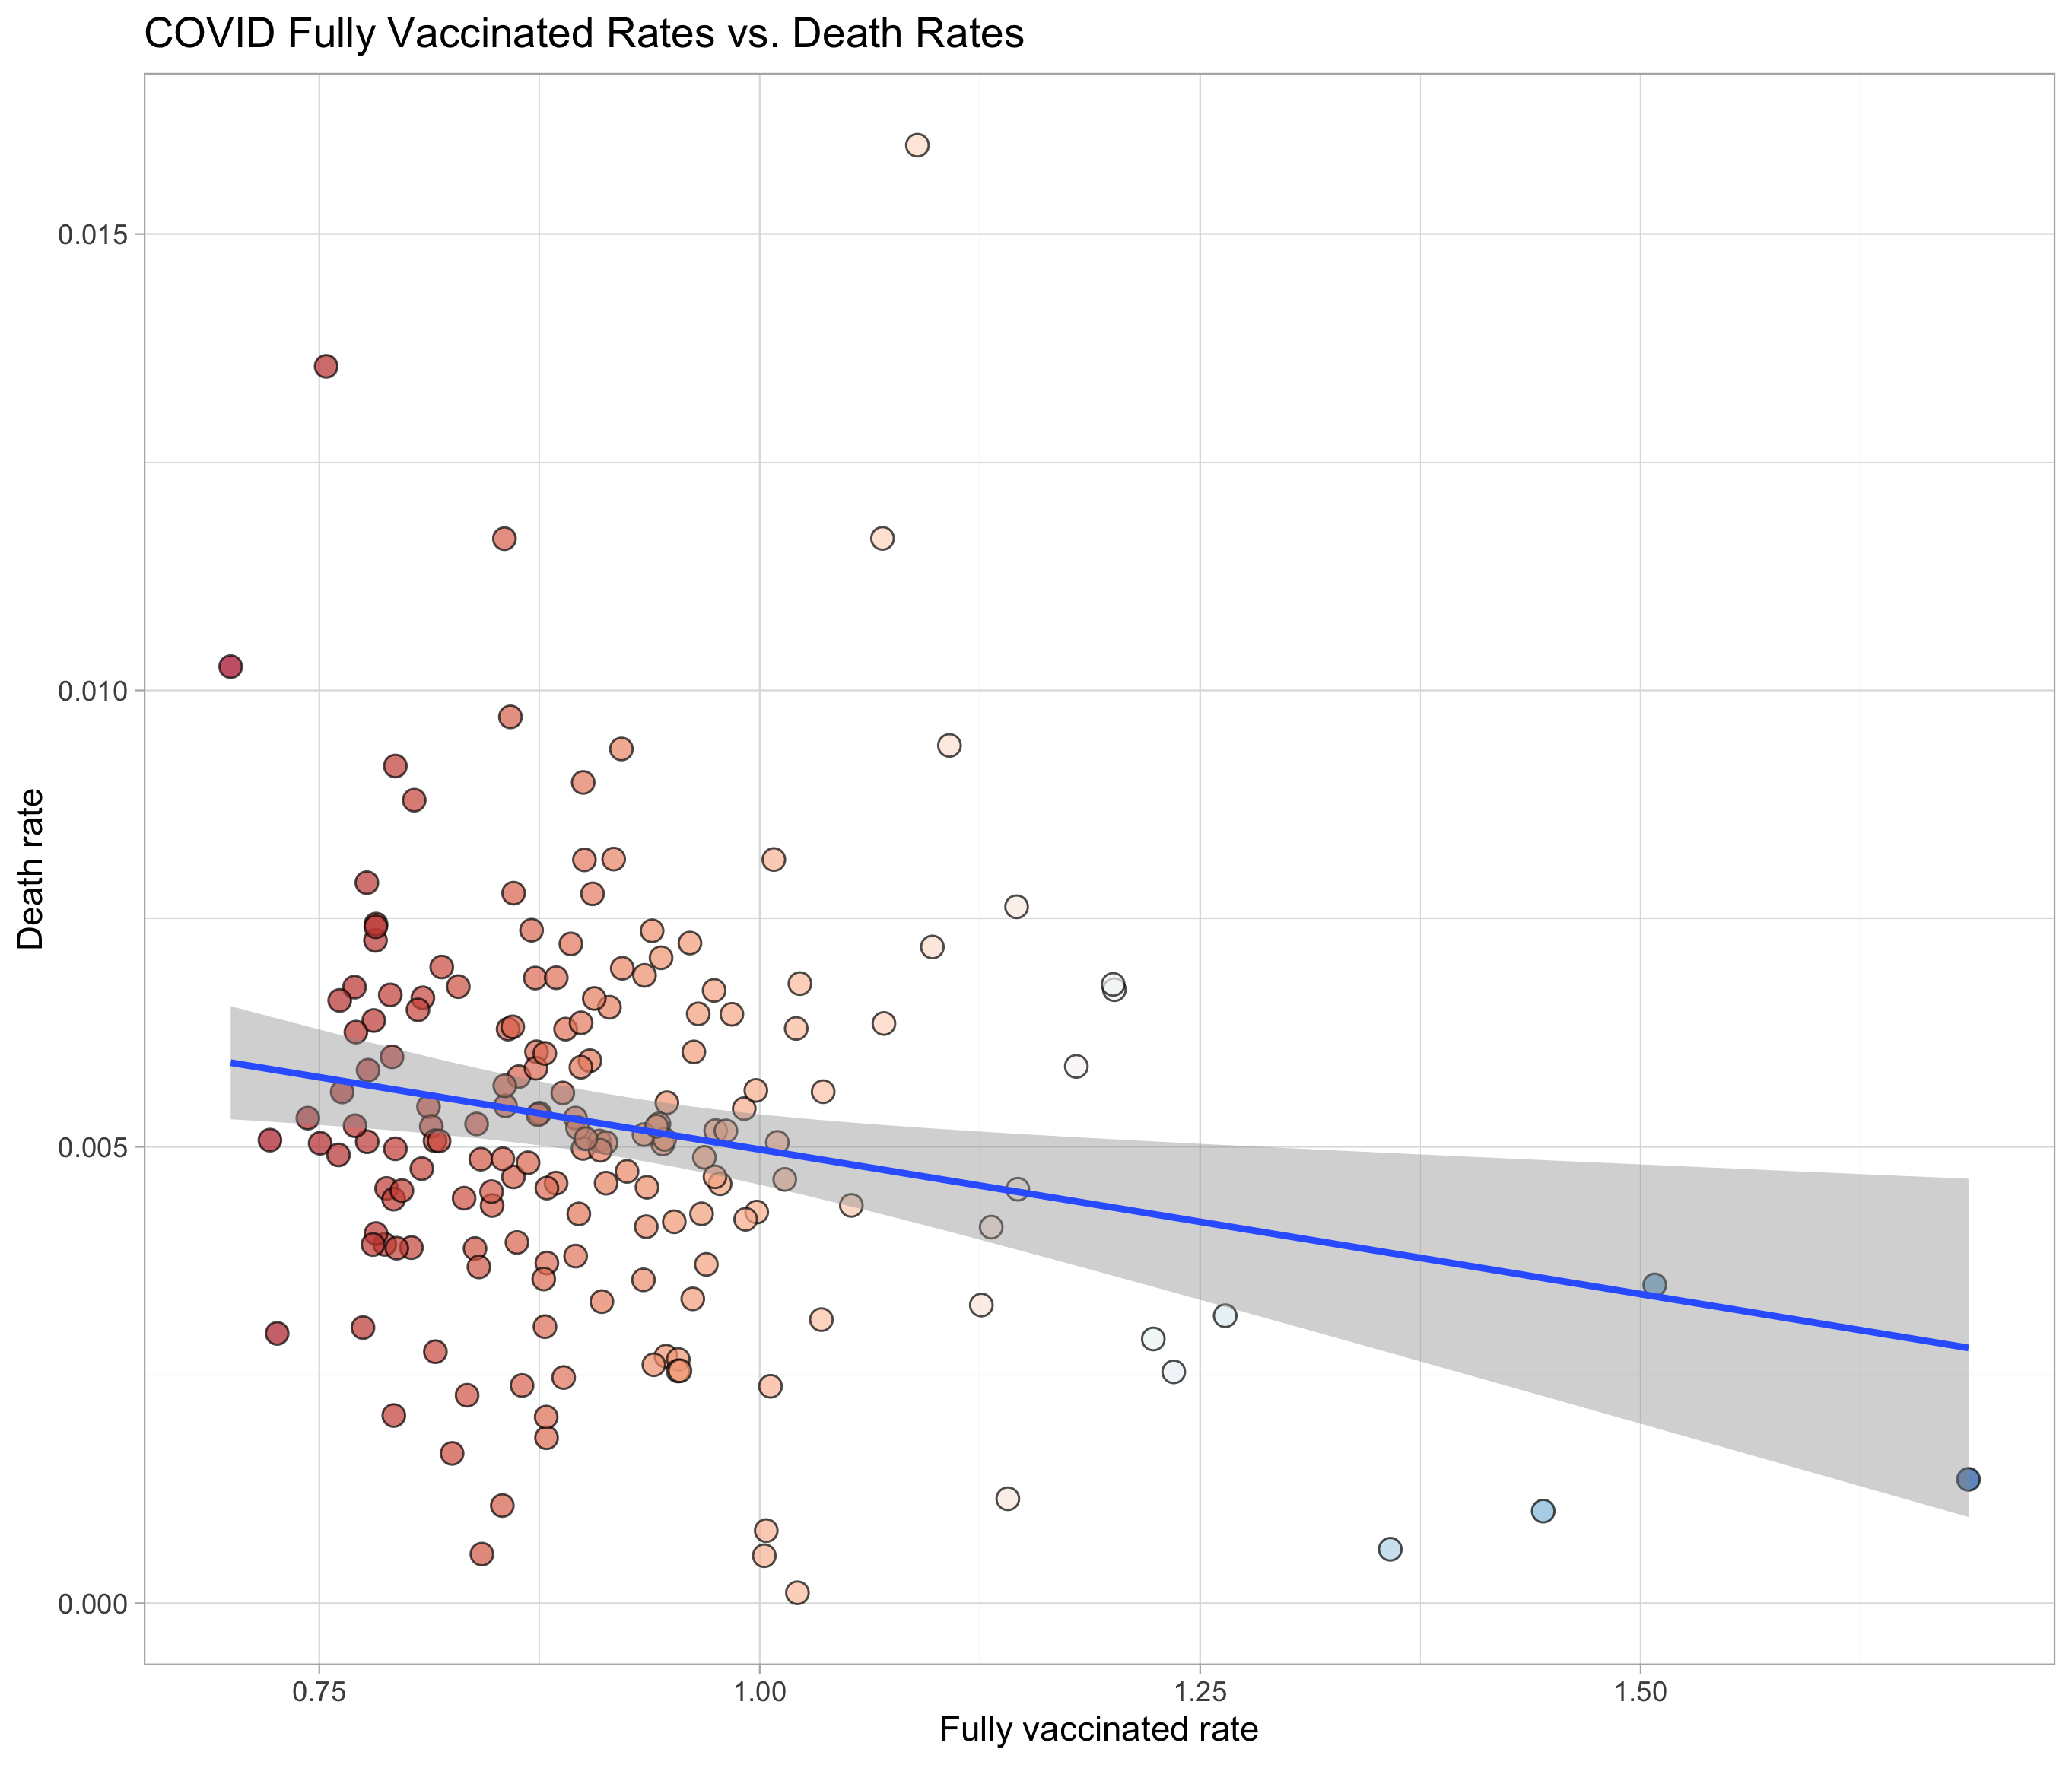
\includegraphics[width=0.25\linewidth]{out/correlations/corr_plot_vax_rates_v_death_rate.png}} 
    \caption{Correlation plots}
    \label{fig:corr}
\end{figure*}

\subsection{Areal Analysis}

\subsubsection{Moran's I and Correlogram Lag Structures}

To understand the spatial dependencies in the data, we performed Moran's I analysis and examined correlogram lag structures.

Moran's I is a measure of spatial autocorrelation, indicating the degree to which a variable is similar to itself in nearby locations. We calculated Moran's I for various metrics using different spatial weights: Queen contiguity, six nearest neighbors (6-NN), and inverse distance weighting (IDW). Results of Moran's I can be seen in table \ref{tab:moran_results}.

\begin{table}[h]
    \centering
    \begin{tabular}{|l|l|r|r|}
        \hline
        \textbf{Method} & \textbf{Metric} & \textbf{Statistic} & \textbf{P-value} \\
        \hline
        Queen & Case Rate & 8.5820 & 4.6627e-18 \\
        Queen & Death Rate & 8.5888 & 4.3948e-18 \\
        Queen & Percent Fully Vaccinated & 7.9847 & 7.0413e-16 \\
        Queen & Dem Fraction 2020 & 9.6518 & 2.416e-22 \\
        Queen & Dem Fraction 2024 & 8.6571 & 2.4186e-18 \\
        IDW & Case Rate & 10.7632 & 2.5686e-27 \\
        IDW & Death Rate & 11.2114 & 1.7932e-29 \\
        IDW & Percent Fully Vaccinated & 6.1612 & 3.6087e-10 \\
        IDW & Dem Fraction 2020 & 14.9204 & 1.2136e-50 \\
        IDW & Dem Fraction 2024 & 12.1339 & 3.4901e-34 \\
        6-NN & Case Rate & 10.7859 & 2.0074e-27 \\
        6-NN & Death Rate & 11.1769 & 2.644e-29 \\
        6-NN & Percent Fully Vaccinated & 9.9011 & 2.0588e-23 \\
        6-NN & Dem Fraction 2020 & 13.0456 & 3.3644e-39 \\
        6-NN & Dem Fraction 2024 & 10.5155 & 3.665e-26 \\
        \hline
    \end{tabular}
    \caption{\centering Moran's I Results for Different Metrics and Methods}
    \label{tab:moran_results}
\end{table}

Correlograms were generated to visualize the autocorrelative effects across neighboring regions using the 6-NN spatial weight, which we observed to be overall the best. Lag plots can be viewed in figure \ref{fig:lag}.

\begin{itemize}
    \item \textbf{Case Rates}: Neighbor effects were observed up to lag 2, indicating that case rates are autocorrelated within two neighboring regions.
    \item \textbf{Death Rates}: Due to the low death rates, autocorrelation extended up to lag 6, showing spatial dependencies up to six neighboring regions.
    \item \textbf{Vaccination Rates}: Similar to case rates, vaccination rates showed autocorrelation within 1-2 lag distances.
    \item \textbf{Voting Fraction 2020}: Autocorrelation was observed up to lag 3, indicating spatial dependencies within three neighboring regions.
    \item \textbf{Voting Fraction 2024}: Similar to 2020, autocorrelation extended up to lag 3.
\end{itemize}

\begin{figure*}[t]
    \centering
    \subfloat[\centering Case Rates]{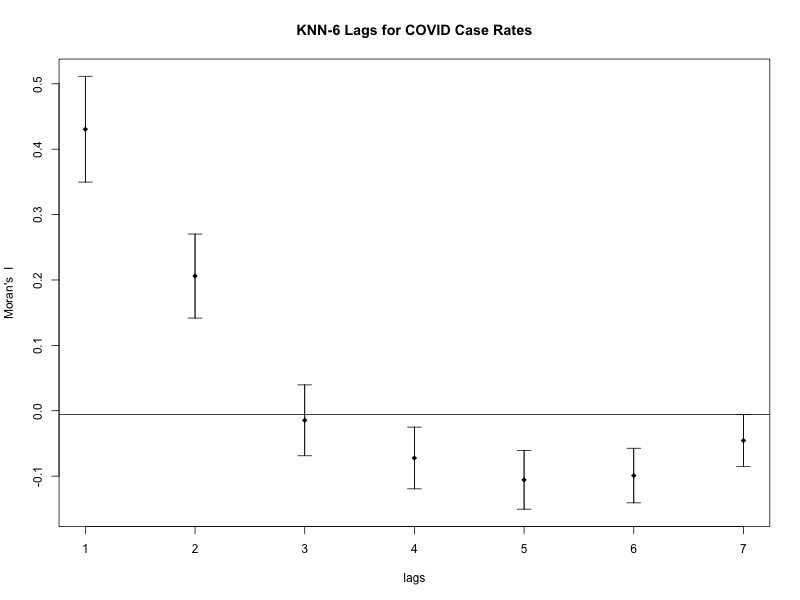
\includegraphics[width=0.25\linewidth]{out/areal/case_rates_lag_plot.png}}
    \subfloat[\centering Death Rates]{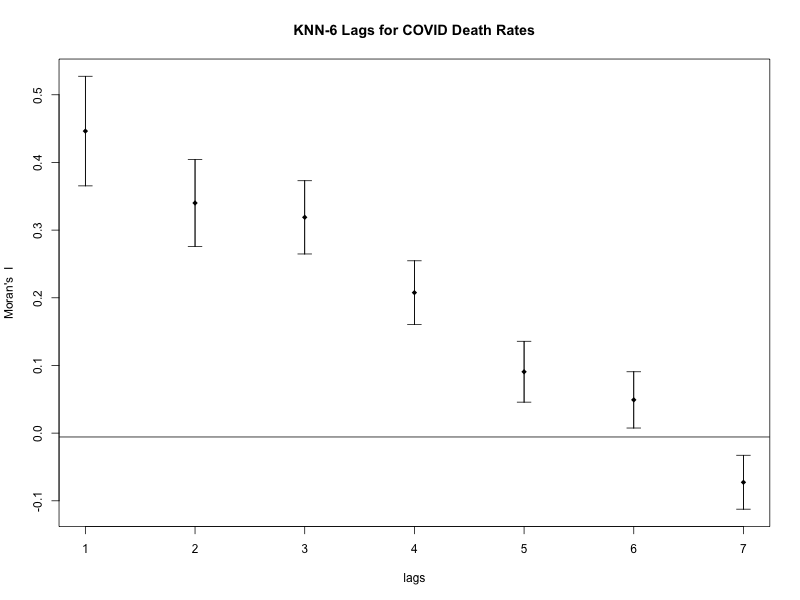
\includegraphics[width=0.25\linewidth]{out/areal/death_rates_lag_plot.png}}
    \subfloat[\centering Vaccination Rates] {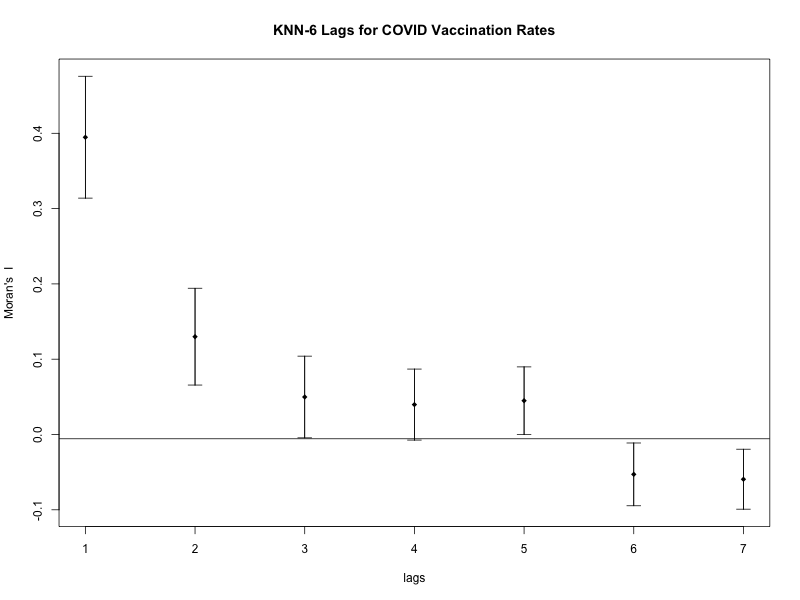
\includegraphics[width=0.25\linewidth]{out/areal/vax_rates_lag_plot.png}} \\
    \subfloat[\centering Dem Fraction 2020]{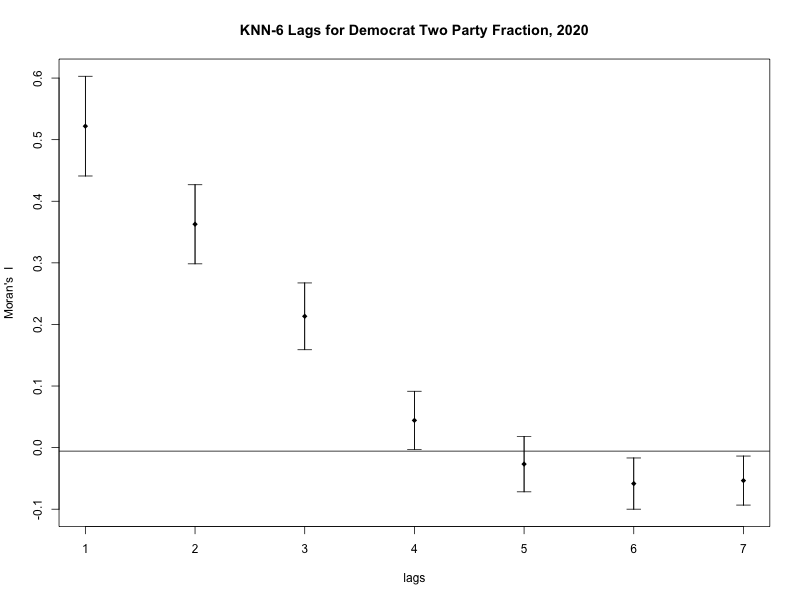
\includegraphics[width=0.25\linewidth]{out/areal/dem_2020_lag_plot.png}}
    \subfloat[\centering Dem Fraction 2024]{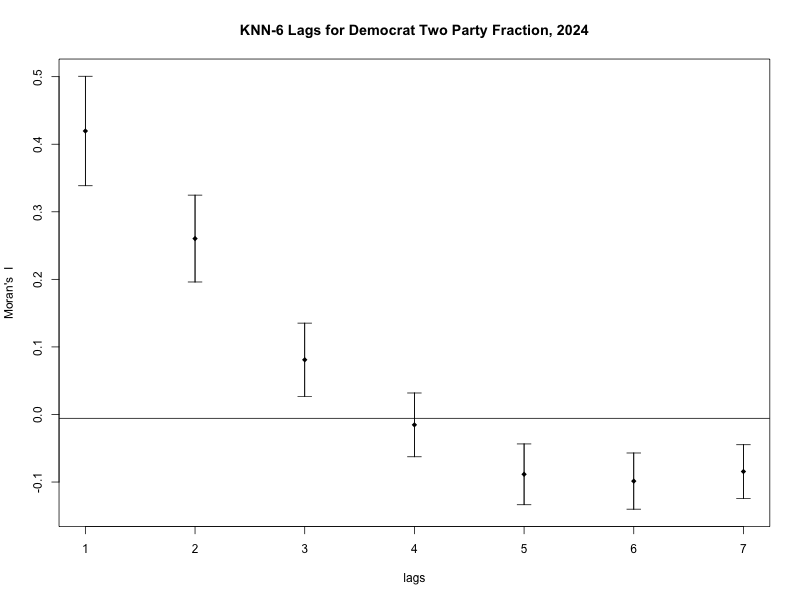
\includegraphics[width=0.25\linewidth]{out/areal/dem_2024_lag_plot.png}} \\
    \subfloat[\centering GOP Fraction 2020]{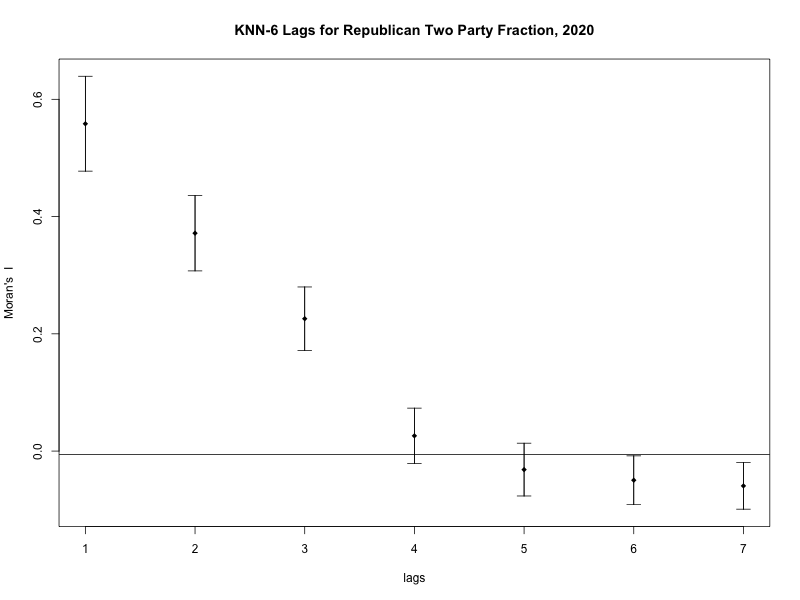
\includegraphics[width=0.25\linewidth]{out/areal/rep_2020_lag_plot.png}} 
    \subfloat[\centering GOP Fraction 2024]{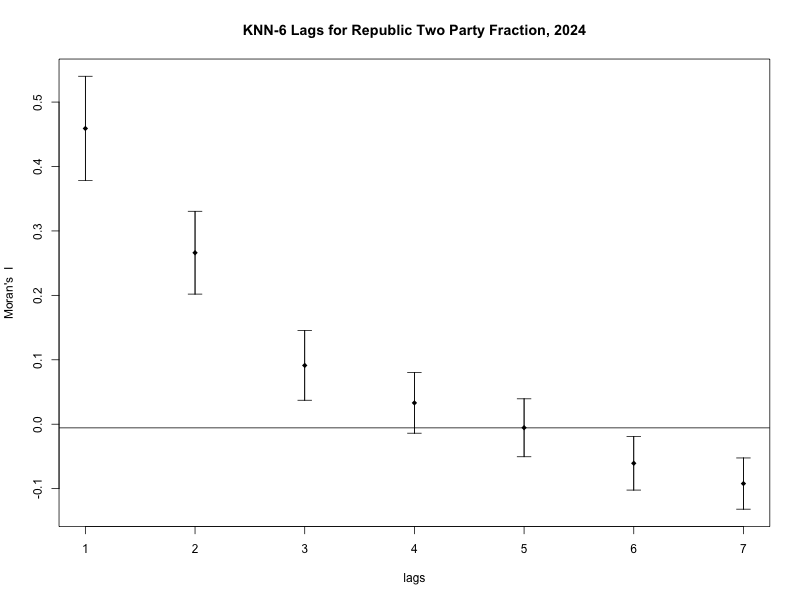
\includegraphics[width=0.25\linewidth]{out/areal/rep_2024_lag_plot.png}}
    \caption{Lag plots}
    \label{fig:lag}
\end{figure*}

\subsubsection{Getis-Ord G-star}

The Getis-Ord Gi* statistic is used to identify clusters of high or low values in spatial data, helping to detect hotspots and cold spots within the dataset. This analysis provides insights into the spatial distribution of COVID-19 metrics and political alignment.

Based on the maps (Fig. \ref{fig:g-star}) we observe the following:
\begin{itemize}
    \item \textbf{Case Rates}: The analysis shows clustering of hotspots in Midtown Manhattan and Staten Island, indicating areas with significantly higher case rates.
    \item \textbf{Death Rates}: Clustering of higher death rates is observed in southern Queens, highlighting regions with elevated mortality.
    \item \textbf{Vaccination Rates}: Hotspots for vaccination rates are also found in Midtown Manhattan, suggesting areas with higher vaccine uptake.
    \item \textbf{Political Alignment (2020 and 2024)}: The analysis reveals clustering of Republican voters in southern Staten Island, Brooklyn, and Queens in 2020, with these clusters migrating north in 2024.
\end{itemize}

\begin{figure*}[t]
    \centering
    \subfloat[\centering Case Rates]{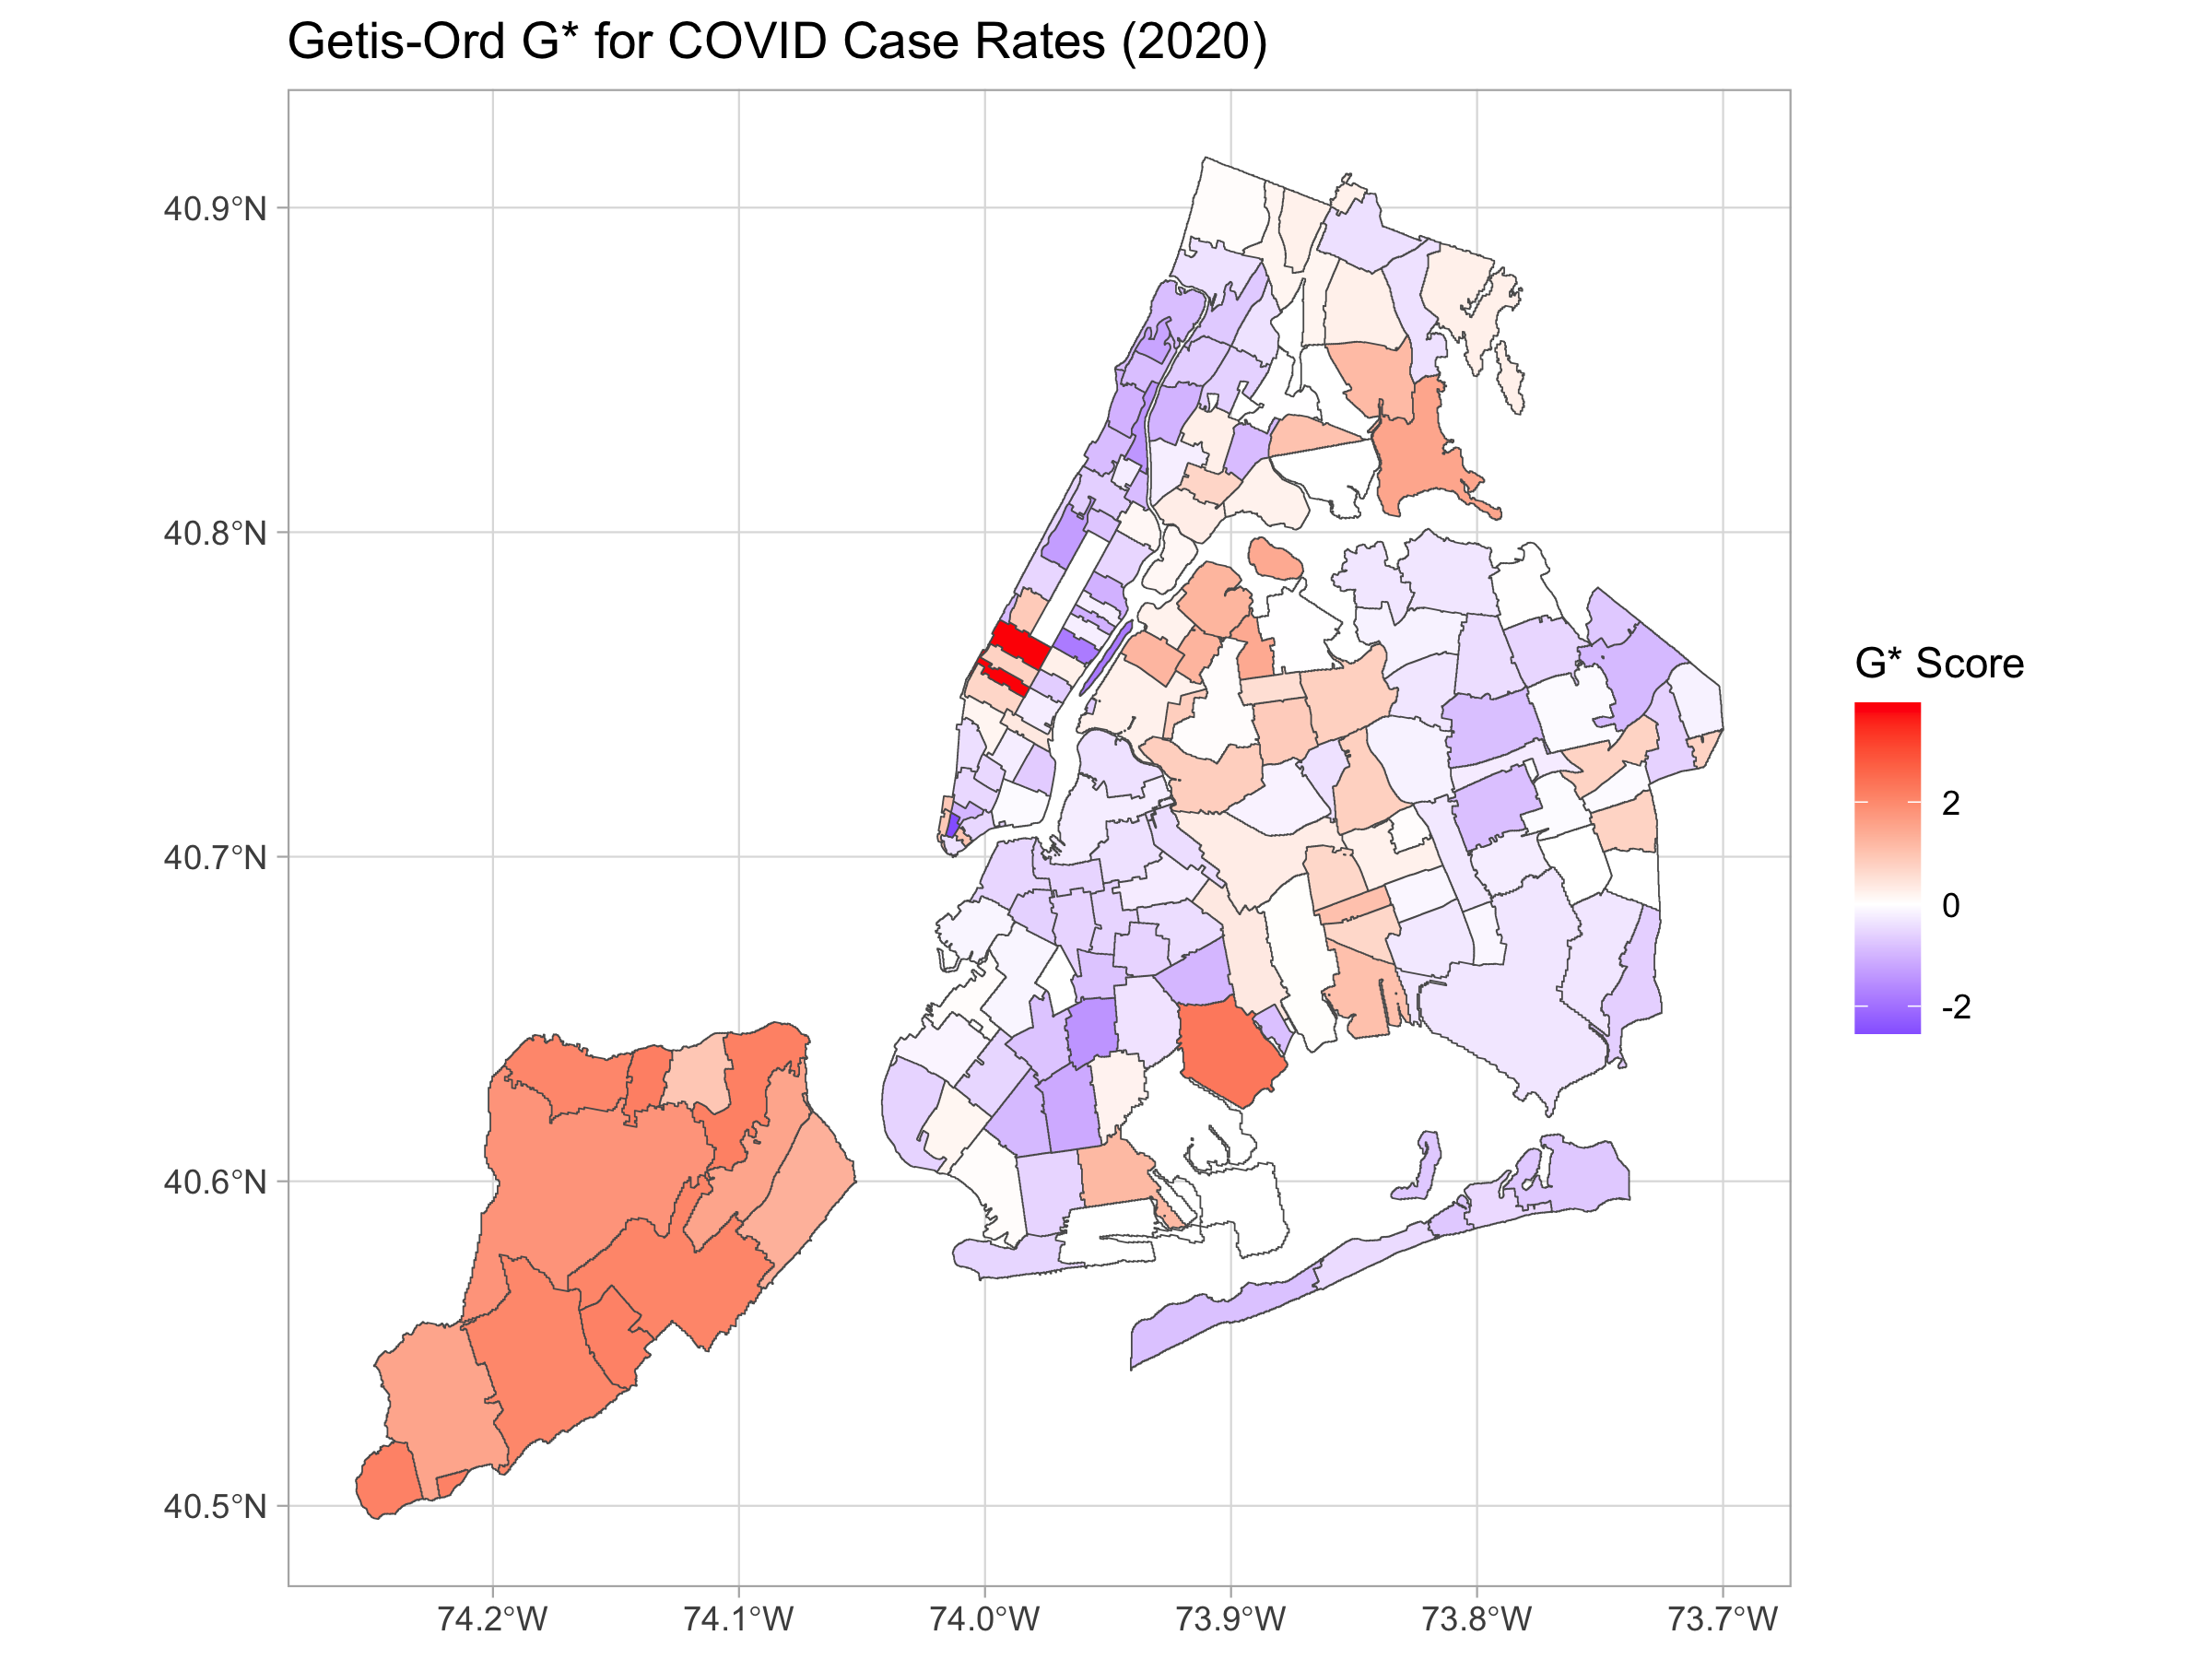
\includegraphics[width=0.3\linewidth]{out/areal/g_star_case_rate_2020.png}}
    \subfloat[\centering Death Rates]{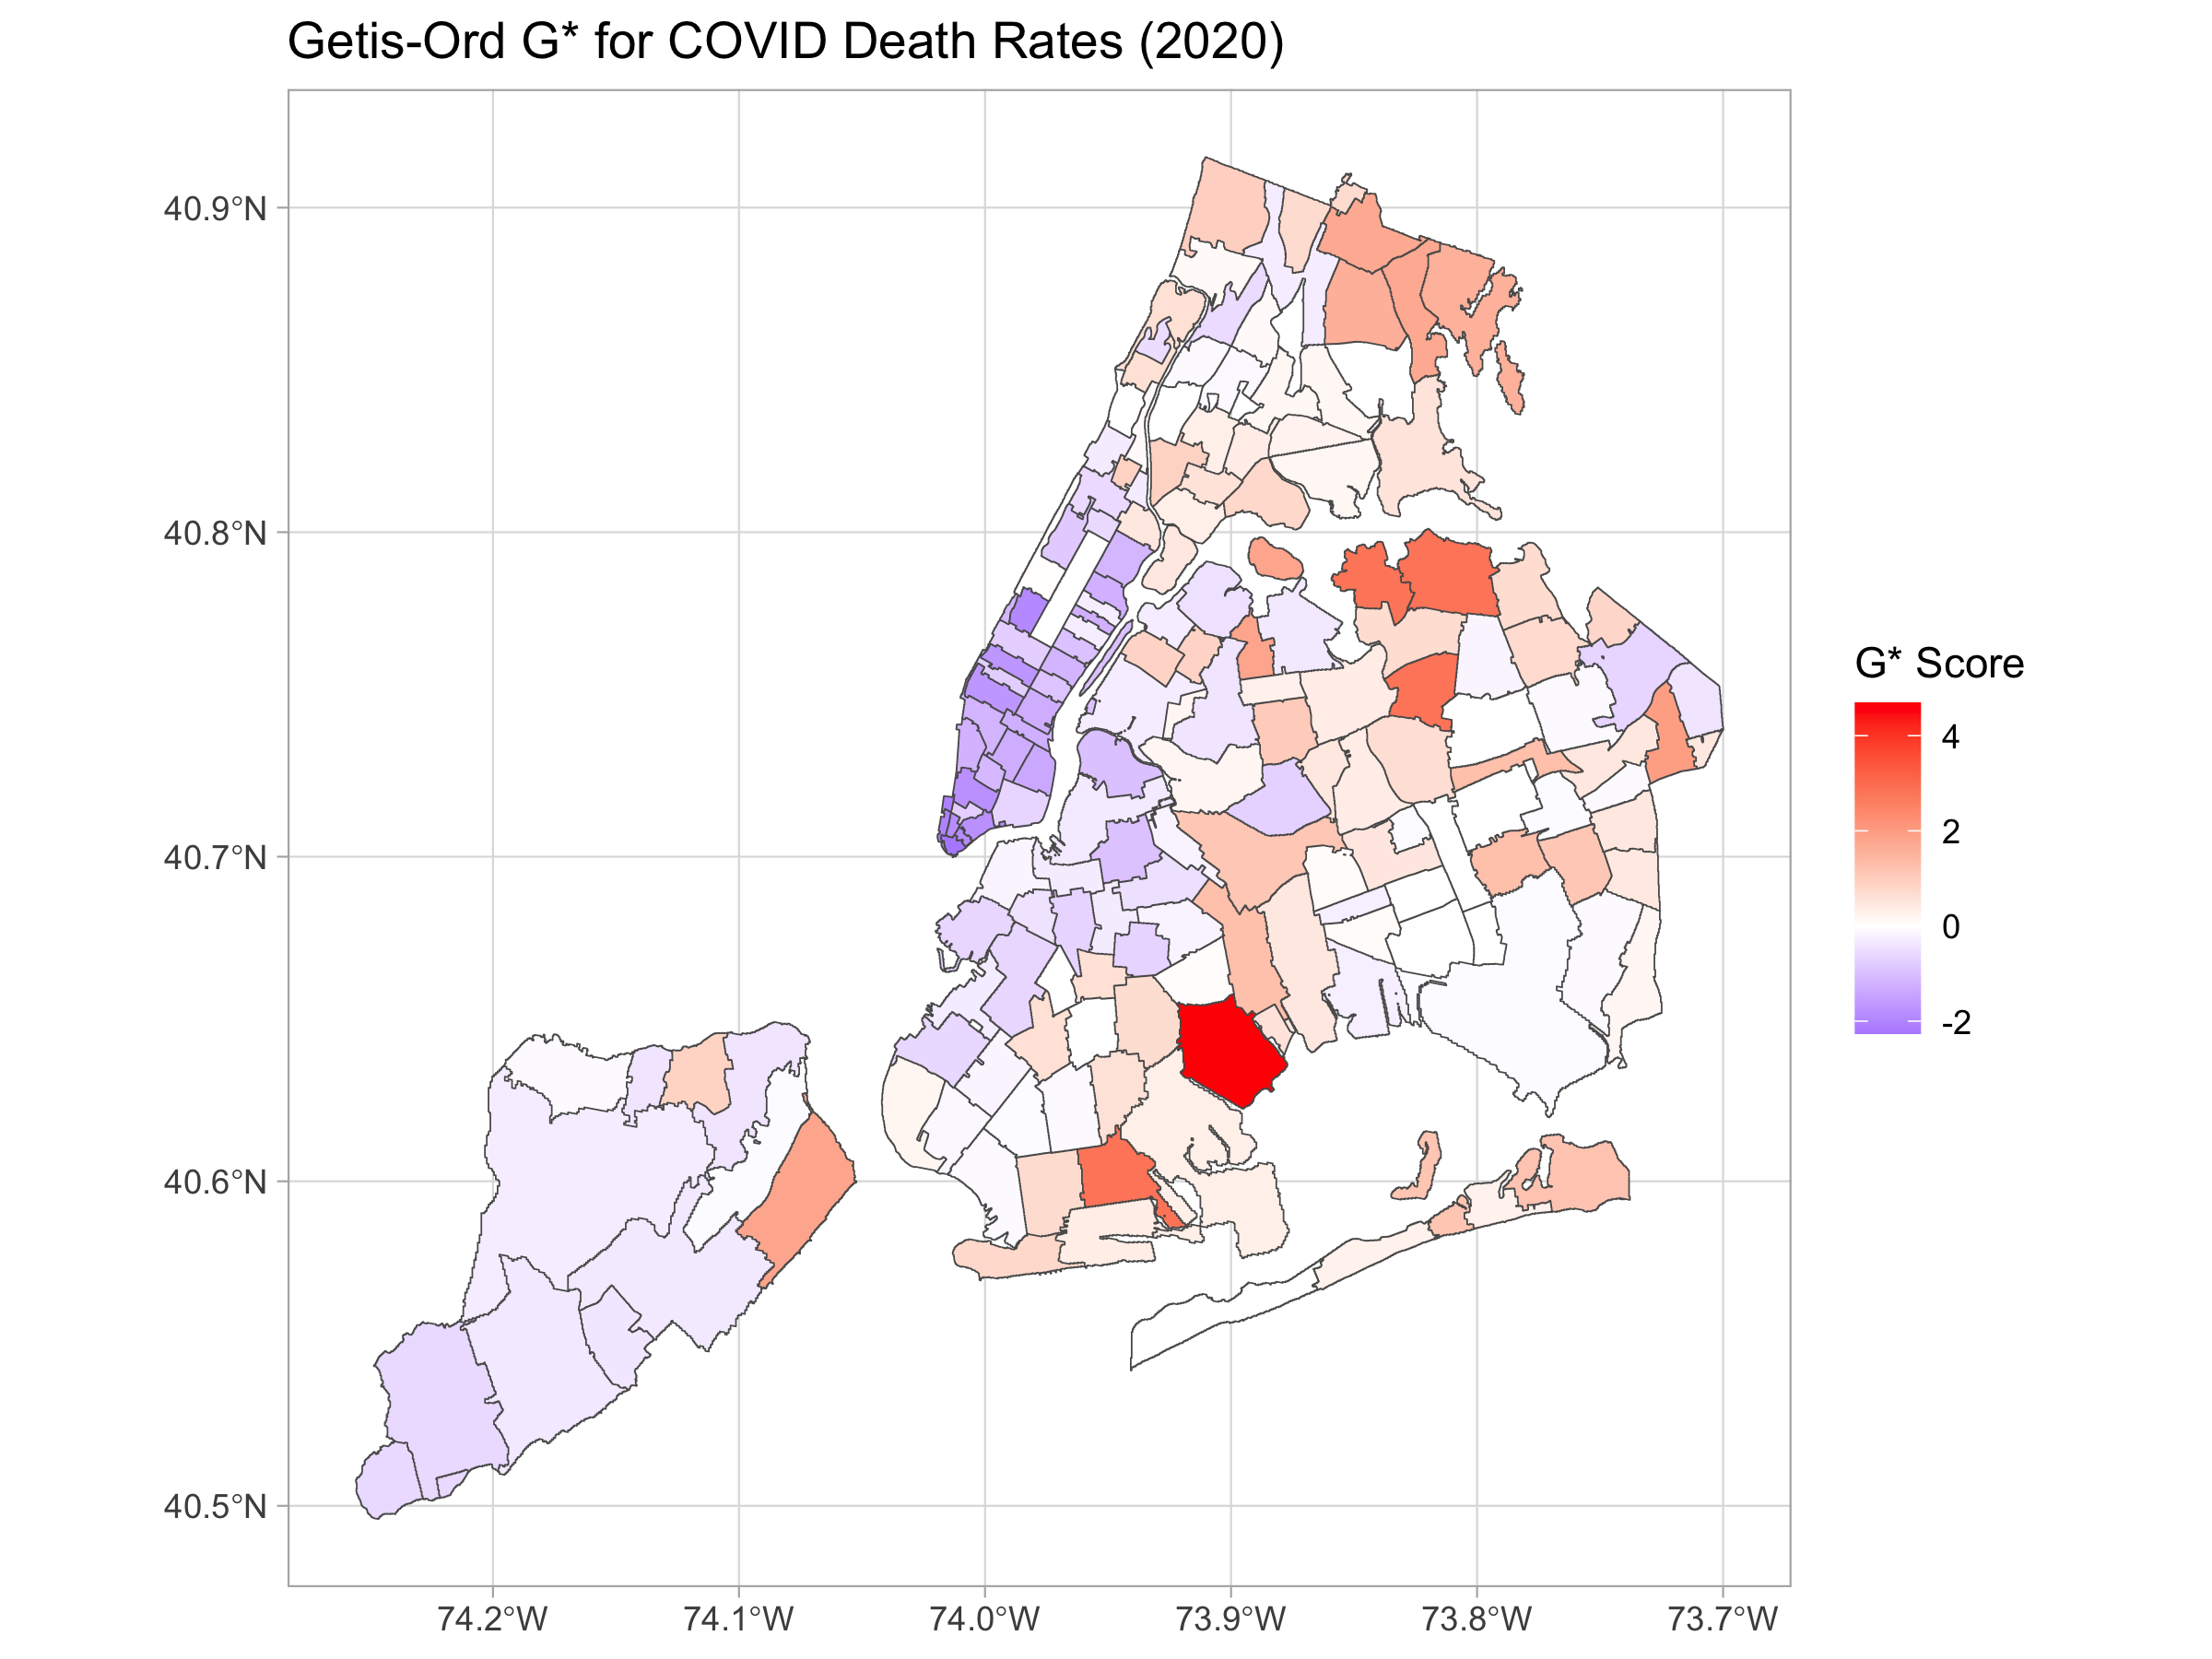
\includegraphics[width=0.3\linewidth]{out/areal/g_star_death_rate_2020.png}}
    \subfloat[\centering Vaccination Rates] {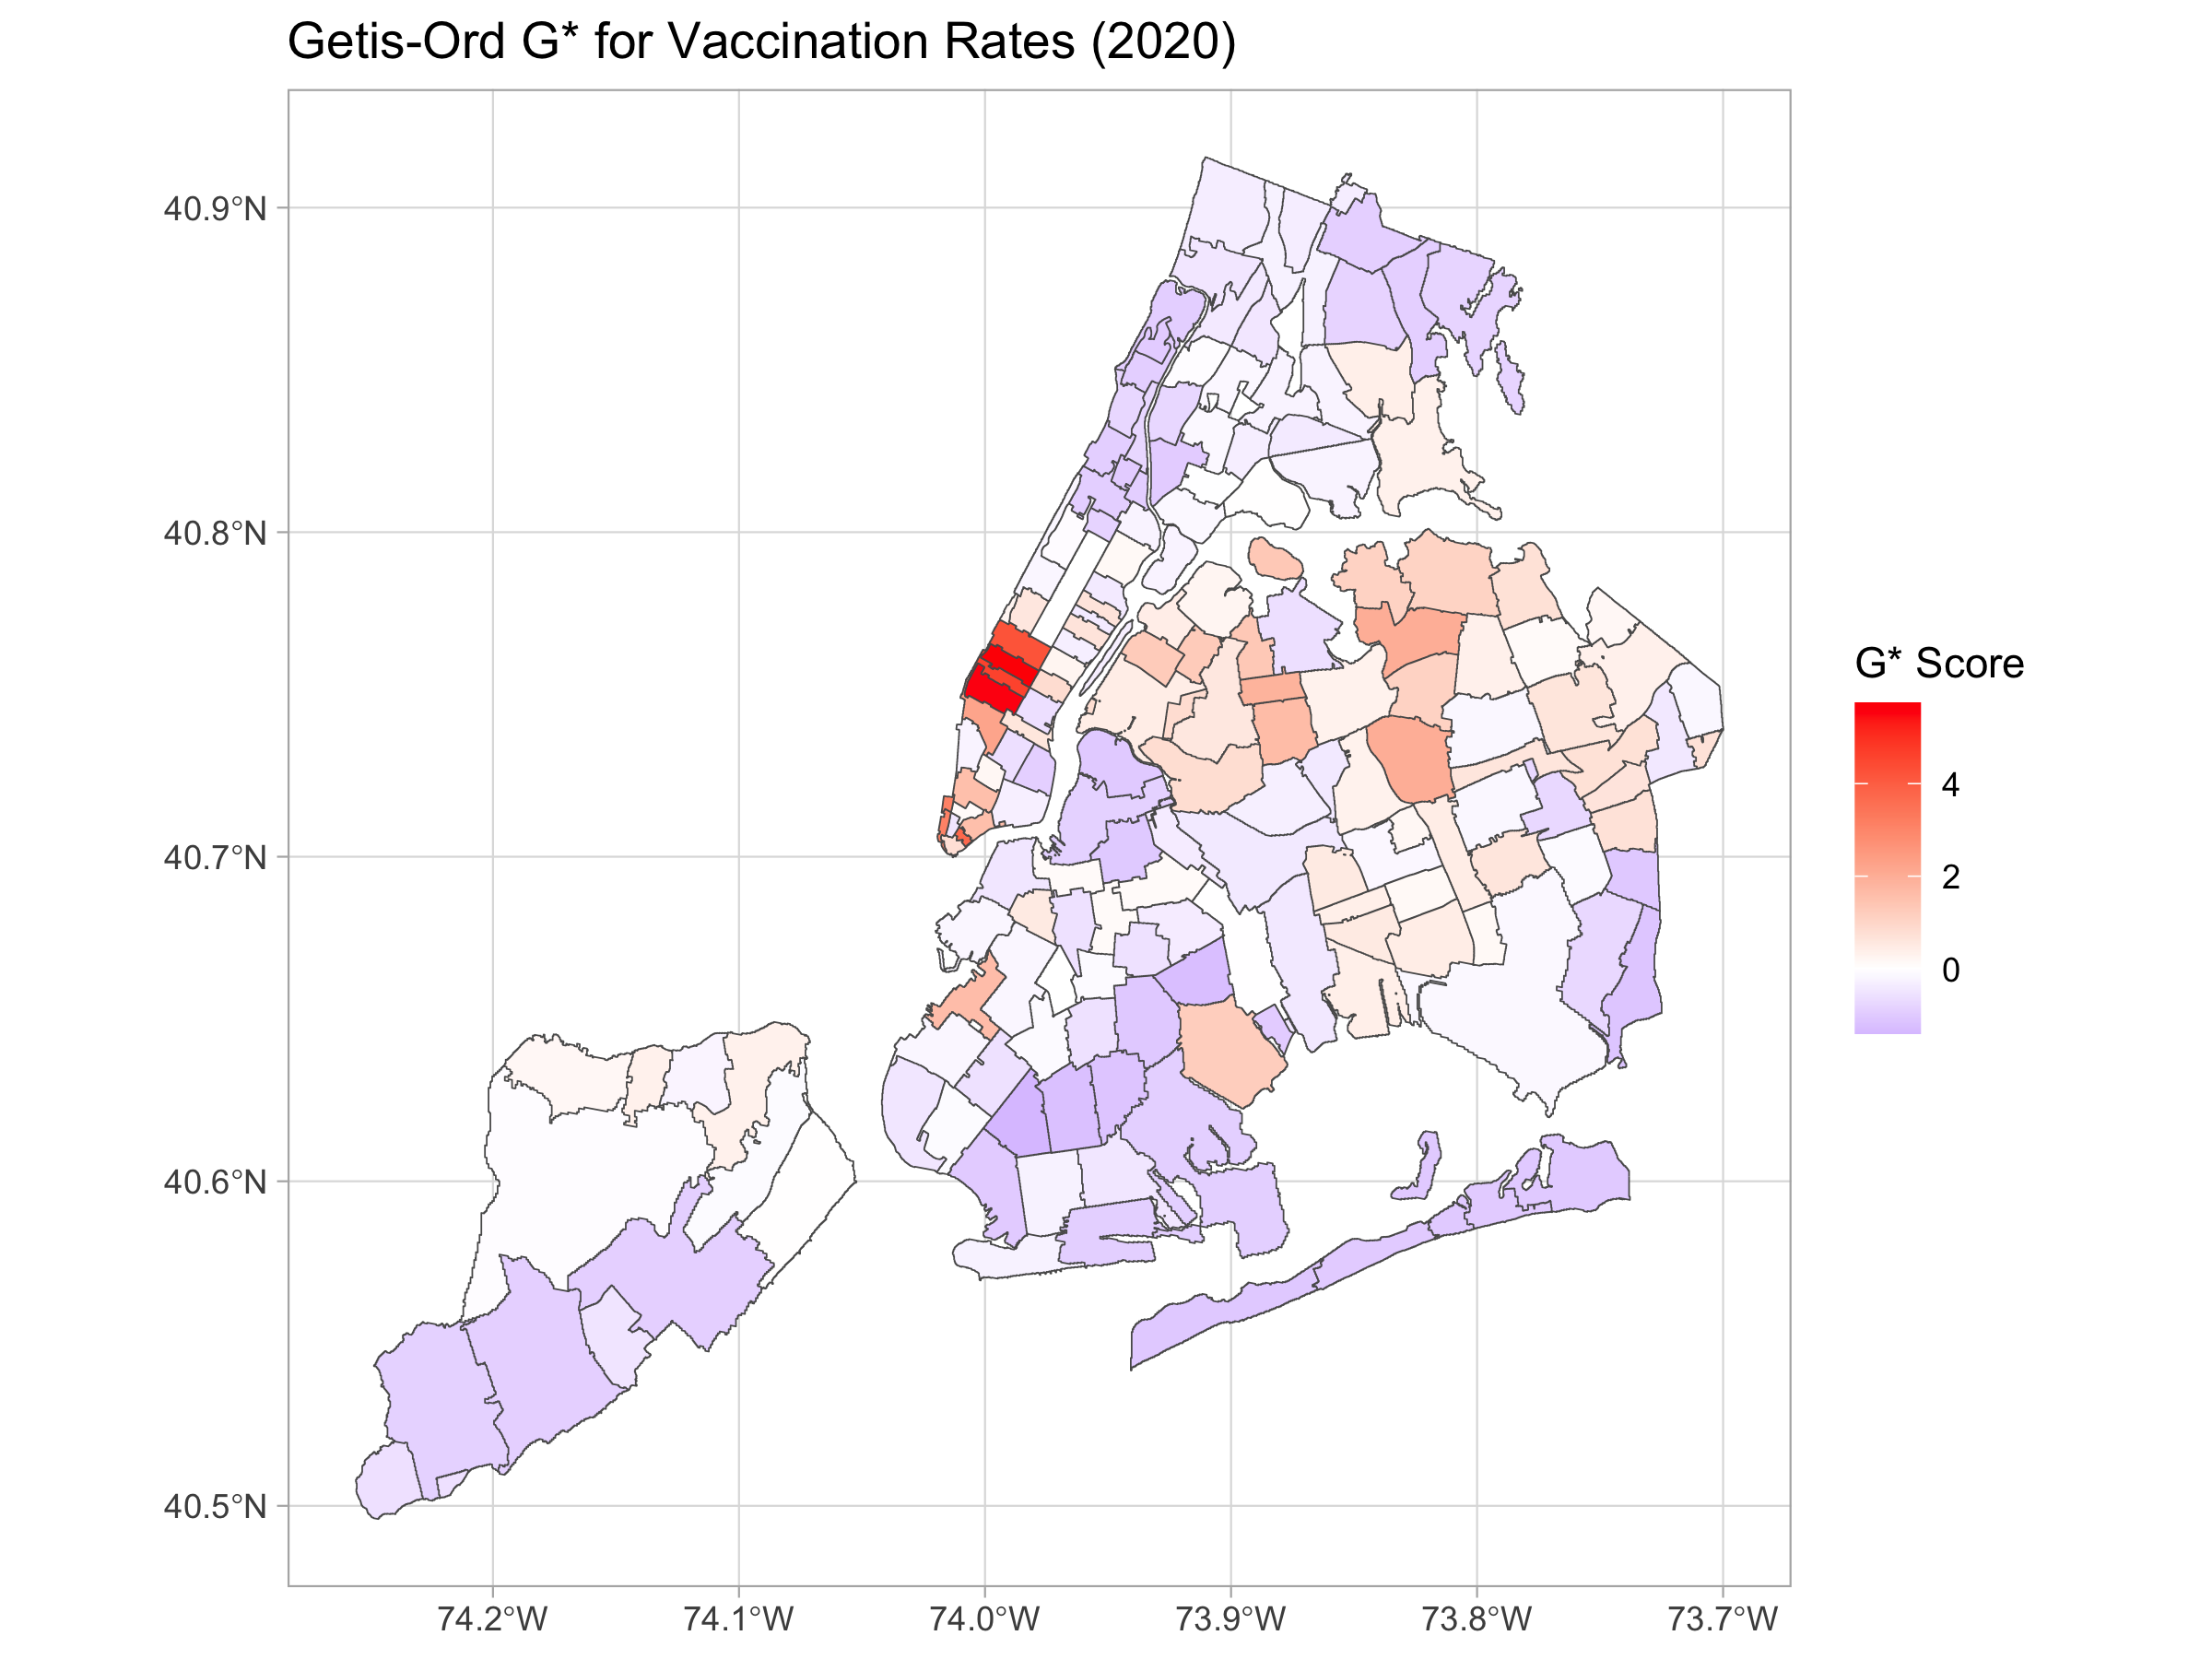
\includegraphics[width=0.3\linewidth]{out/areal/g_star_vax_rate_2020.png}} \\
    \subfloat[\centering Dem Fraction 2020]{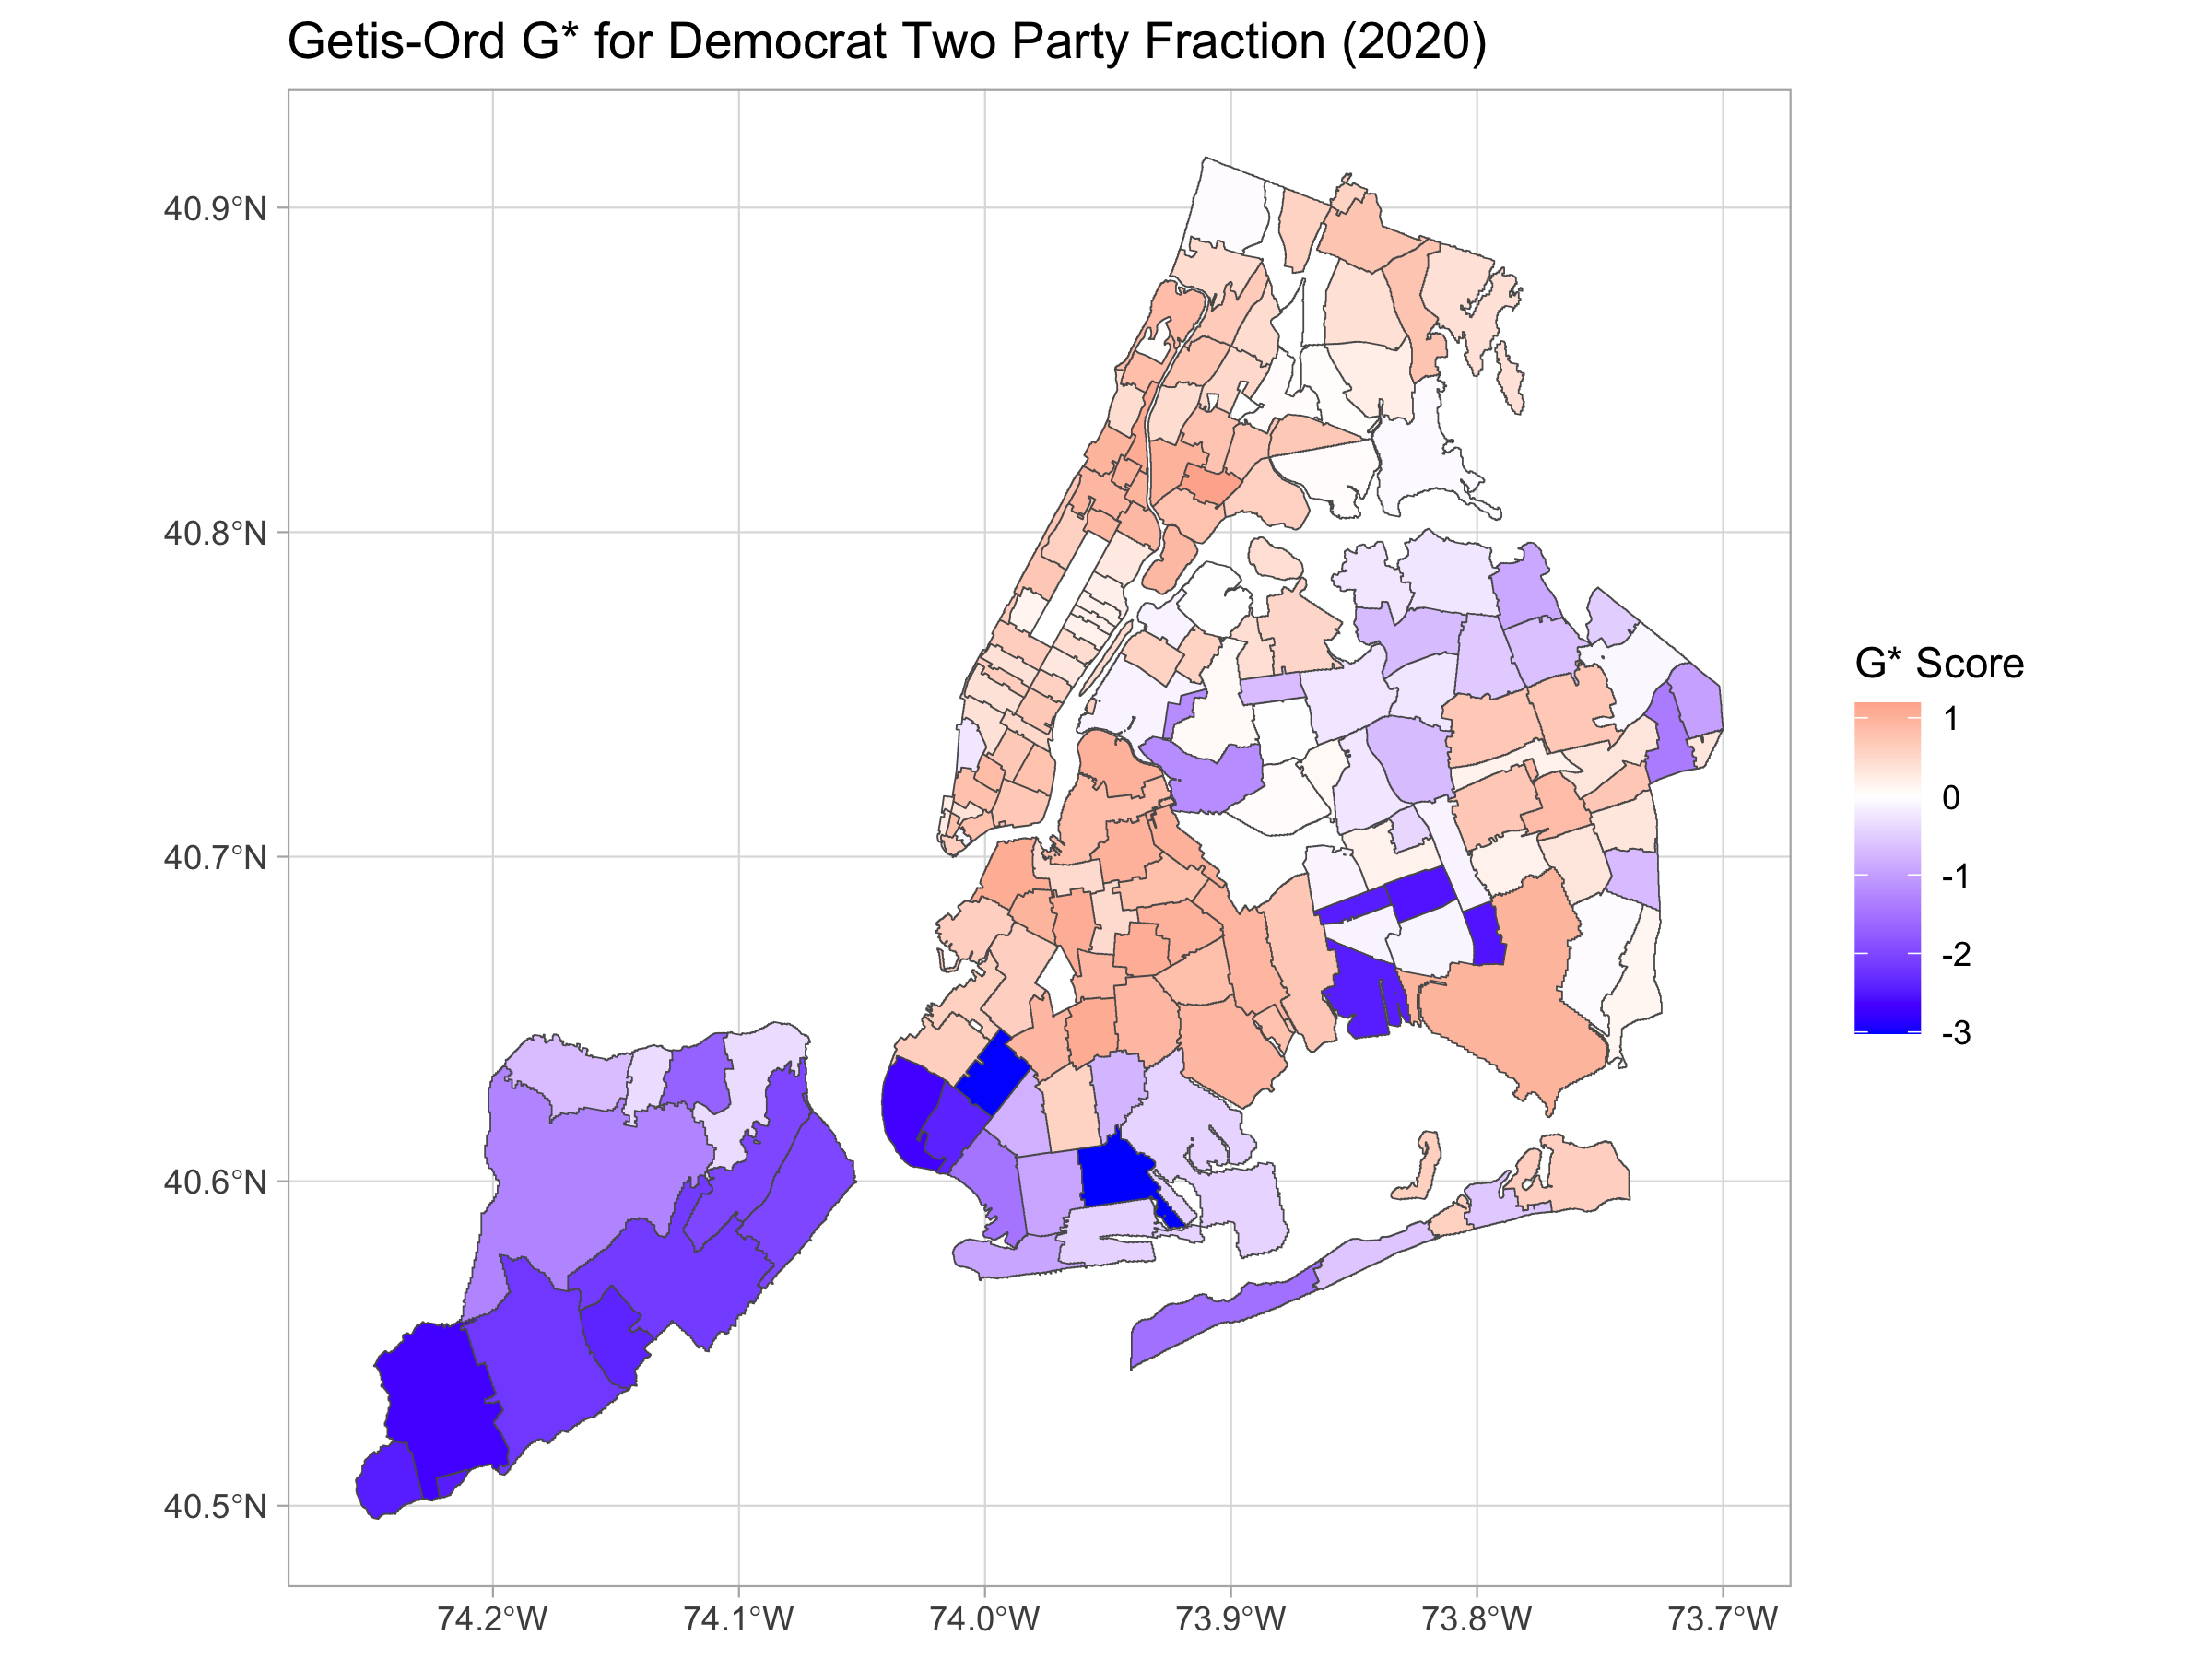
\includegraphics[width=0.3\linewidth]{out/areal/g_star_dem_2020.png}}
    \subfloat[\centering Dem Fraction 2024]{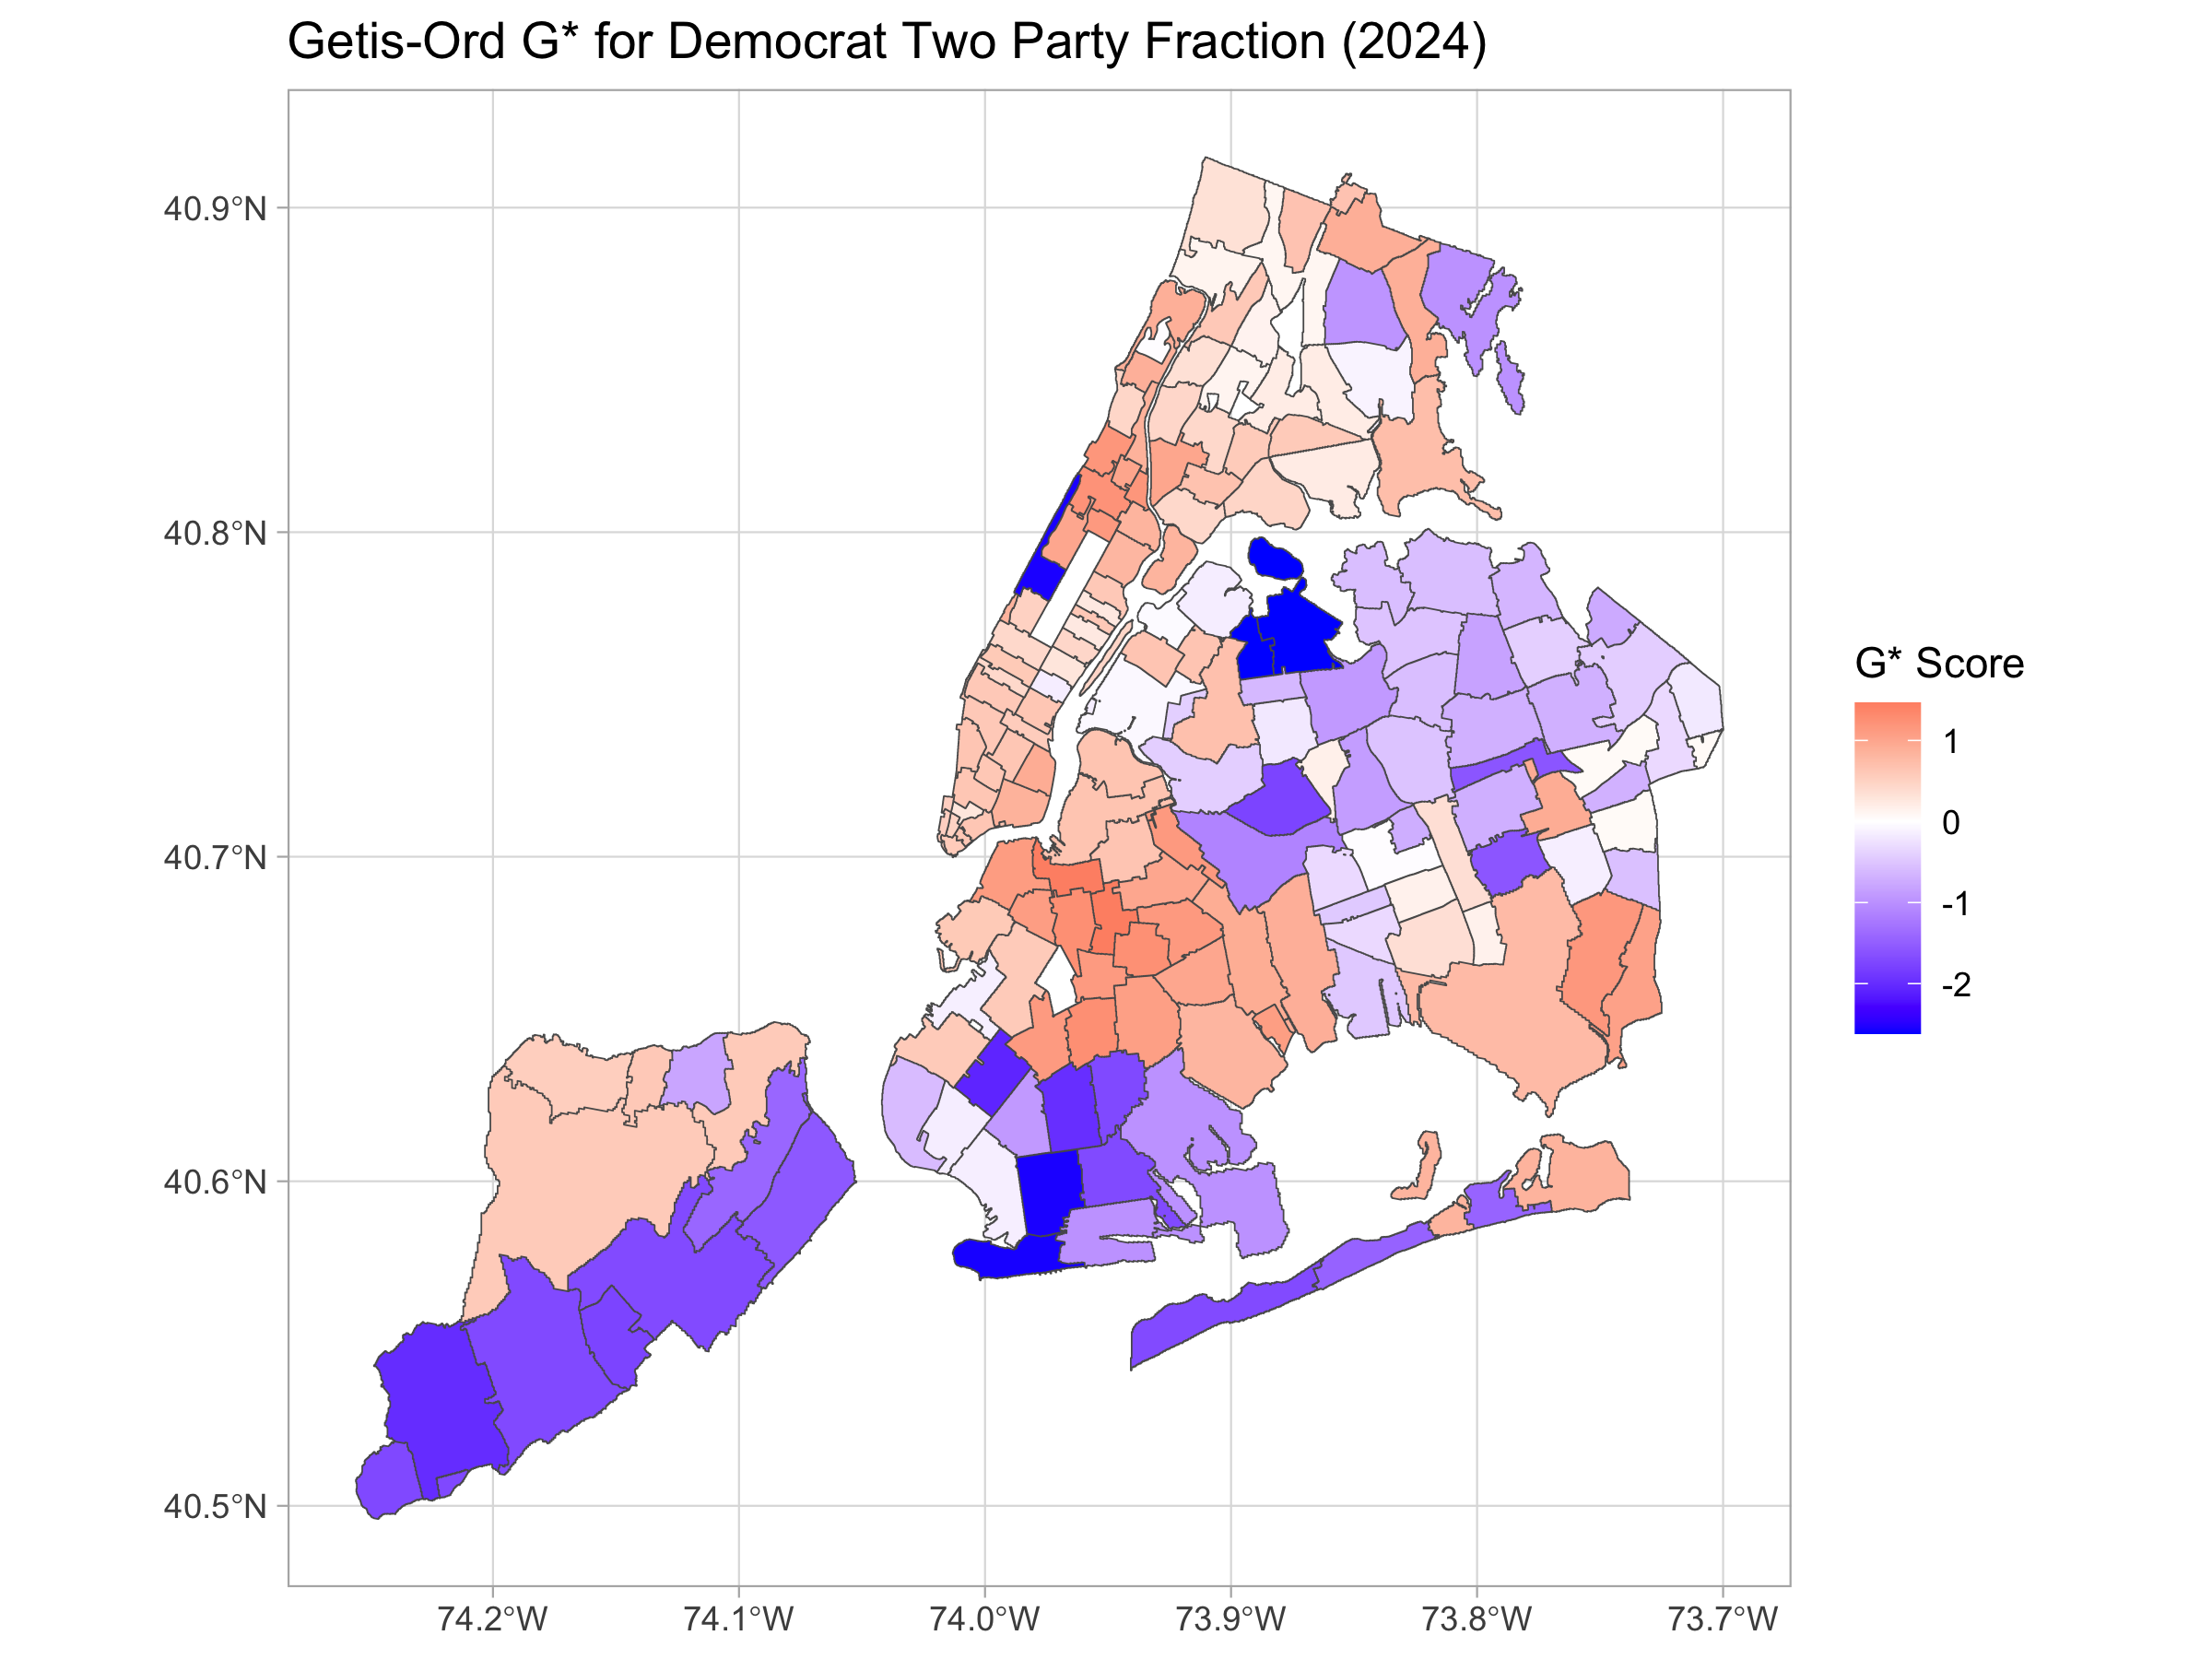
\includegraphics[width=0.3\linewidth]{out/areal/g_star_dem_2024.png}}
    \caption{Getis-Ord Gi* Mappings}
    \label{fig:g-star}
\end{figure*}

\subsection{SAR and CAR Models}

To account for spatial dependencies, we applied both the Spatial Autoregressive (SAR) model and the Conditional Autoregressive (CAR) model to analyze the relationship between COVID-19 case rates, vaccination rates, and political alignment.

The SAR model incorporates spatial lag-errors to capture the influence of neighboring regions on the variable of interest. However, in the analysis, the CAR model considers the conditional distribution of each region given its neighbors, providing a better fit for irregular spatial layouts (Table \ref{tab:sar_car_results}).

\begin{table}[h]
    \centering
    \begin{tabular}{|l|l|r|r|}
        \hline
        \textbf{Model} & \textbf{Variable} & \textbf{Estimate} & \textbf{P-value} \\
        \hline
        SAR & Intercept & -3.46721 & 1.724e-11 \\
        SAR & Democrat Fraction & -0.11151 & 0.7111 \\
        SAR & Percent Fully Vaccinated & 4.06339 & $<$ 2.2e-16 \\
        SAR & AIC & 368.21 & - \\
        CAR & Intercept & 15.875 & $<$ 2.2e-16 \\
        CAR & Democrat Fraction & 9.1847 & $<$ 2.2e-16 \\
        CAR & Percent Fully Vaccinated & 12.666 & $<$ 2.2e-16 \\
        CAR & AIC & -1681.7 & - \\
        \hline
    \end{tabular}
    \caption{SAR and CAR Model Results}
    \label{tab:sar_car_results}
\end{table}

The SAR model shows that case rates and vaccination rates capture most of the spatial behavior, but not voting behavior, with an AIC of 368.21. The CAR model, with an AIC of -1681.7, indicates that vaccination rates and voting fractions better capture the autoregressive behavior in COVID case rates, making it more suitable for the irregular spatial layouts of NYC in this particular context.

\section{Conclusion}

This study aimed to explore the relationship between political alignment and COVID-19 outcomes, including case rates, death rates, and vaccination rates, across New York City neighborhoods. Despite showing no significant correlation between vaccination rates and political alignment, we observed a negative correlation between Democrat voters and COVID-19 case rates, and a positive correlation for Republican voters. This indicates that areas with higher Republican support experienced higher case rates. Similarly, death rates were negatively correlated with Democrat voters.

The Moran's I analysis and correlogram lag structures revealed significant spatial autocorrelation for COVID-19 metrics and political alignment. The 6-NN method provided the best results, due to the irregular spatial shape of the MODZCTA regions and due to the local geography. Additionally, the CAR model outperformed the SAR model, capturing the autoregressive behavior in COVID-19 case rates more effectively. This indicates that the CAR model is better suited for the irregular spatial layouts of NYC. However, we only explored two relevant features: voting behaviour and vaccination behaviour on COVID-19 case rates, and future work may want to consider other features as well.

Overall, our findings suggest that political alignment does influence COVID-19 outcomes, particularly case rates and death rates. However, NYC is a large, well-connected, diverse city, and as a result, the interpretability of COVID-19 case rates cannot be simply chalked-up to so few factors. While this work provides initial insights into the relationship between political alignment and COVID-19 outcomes, it also underscores the complexity of the factors at play. Continued research and more comprehensive data are essential to fully understand and address the public health challenges posed by COVID-19 or similar public health emergencies in a dense urban environment like New York City.


% Any acknowledgments to only be included in camera ready
% \ifpeerreview \else
% \section*{Acknowledgments}
% The authors would like to thank...
% \fi

\bibliographystyle{IEEEtran}
\bibliography{references}



% \ifpeerreview \else
%%%% For the camera ready version, please fill out this
%%%% biography. Your camera ready should be within a 12 page limit
%%%% including acknowledgments, references and biography.

% If you have an EPS/PDF photo (graphicx package needed) extra braces are
% needed around the contents of the optional argument to biography to prevent
% the LaTeX parser from getting confused when it sees the complicated
% \includegraphics command within an optional argument. (You could
% create your own custom macro containing the \includegraphics command
% to make things simpler here.)
% \begin{IEEEbiography}[{\includegraphics[width=1in,height=1.25in,clip,keepaspectratio]{mshell}}]{Michael Shell}
% or if you just want to reserve a space for a photo:

% \begin{IEEEbiography}{Michael Shell}
% Biography text here.
% \end{IEEEbiography}

% insert where needed to balance the two columns on the last page with
% biographies
%\newpage

% if you will not have a photo at all:
% \begin{IEEEbiographynophoto}{John Doe}
% Biography text here.
% \end{IEEEbiographynophoto}

% You can push biographies down or up by placing
% a \vfill before or after them. The appropriate
% use of \vfill depends on what kind of text is
% on the last page and whether or not the columns
% are being equalized.
%\vfill

% \fi

\end{document}


